\documentclass[11pt,letterpaper]{article}

\usepackage{showlabels}
\usepackage{fullpage}
\usepackage{pslatex}
%\usepackage{latexsym}
\usepackage[english]{babel}
\usepackage[utf8]{inputenc}
\usepackage{amsmath}
\usepackage{bm}
\usepackage{graphicx}
\usepackage{tikz}
\usepackage{xcolor}
\usepackage{url}
%\usepackage[colorinlistoftodos]{todonotes}
\usepackage{rotating}
\usepackage{natbib}
\usepackage{amssymb}

\usepackage{tikz-dependency}
\usepackage{longtable}


\newcommand{\R}[0]{\mathbb{R}}
\newcommand{\E}[0]{\mathbb{E}}
\newcommand{\Ff}[0]{\mathcal{F}}

\usepackage{multirow}

\newcommand{\soft}[1]{}
\newcommand{\nopreview}[1]{}
\newcommand\comment[1]{{\color{red}#1}}
\newcommand\mhahn[1]{{\color{red}(#1)}}

\usepackage{amsthm}

\newcommand{\thetad}[0]{{\theta_d}}
\newcommand{\thetal}[0]{{\theta_{LM}}}

\newcounter{theorem}
\newtheorem{proposition}[theorem]{Proposition}
\newtheorem{thm}[theorem]{Theorem}
\newtheorem{corollary}[theorem]{Corollary}
\newtheorem{question}[theorem]{Question}
\newtheorem{example}[theorem]{Example}
\newtheorem{lemma}[theorem]{Lemma}


\frenchspacing
%\def\baselinestretch{0.975}

%\emnlpfinalcopy
%\def\emnlppaperid{496}

\title{SI}
\author{Michael Hahn, Judith Degen, Richard Futrell}
\date{2019}

\begin{document}

\maketitle


%
\begin{abstract}

Online memory limitations are well-established as a factor impacting sentence processing and have been argued to account for crosslinguistic word order regularities. Building off expectation-based models of language processing, we provide an information-theoretic formalization of these memory limitations. We introduce the idea of a memory-surprisal tradeoff: comprehenders can achieve lower average surprisal per word at the cost of storing more information about past context. We show that the shape of the tradeoff is determined in part by word order. In particular, languages will enable more efficient tradeoffs when they exhibit information locality: when predictive information about a word is concentrated in the word’s recent past. We show evidence from corpora of 52 real languages showing that languages allow for more efficient memory-surprisal tradeoffs than random baseline word order grammars. 

%Are languages optimized for processing with limited memory?
%Memory limitations are well-established as a factor impacting sentence processing, and have been argued to account for crosslinguistic word order regularities.
%Computational models of language processing implementing memory constraints take various forms and make different kinds of assumptions about the architecture underlying human language processing.
%We first  establish general information-theoretic lower bounds on memory that hold in any model of language processing, applying both to speakers and listeners. %assuming only that listeners perform incremental prediction.
%Applying these results to corpora from over 50 languages, we then provide evidence that word orders in human language are optimized for memory demands of speakers and listeners. % producing language and listeners predicting input.
\end{abstract}


%
%
%\begin{thm}\label{prop:suboptimal}
%	For each positive integer $t$, define
%$I_t := I[X_t, X_0 | X_{1\dots t-1}]$,
%i.e., the mutual information between words at distance $t$, controlling for redundancy with the intervening words.
%	Let $T$ be a positive integer, and consider a comprehender using at most $\sum_{t=1}^T t I_t$
%bits of memory on average.
%Then this comprehender will incur average surprisal at least
%	$H[X_t|X_{<t}] + \sum_{t > T} I_t$.
%\end{thm}
%

 
\section{Introduction}

Since the 1950s, it has been a persistent suggestion that human language processing is shaped by a resource bottleneck in short-term memory.
Language is produced and comprehended incrementally in a way that crucially requires both speaker and listener to use an active memory store to keep track of what was previously said.
Since short-term memory of this kind is known to be highly limited in capacity \citep{miller1956magical}, it makes sense for these capacity limits to comprise a major constraint on production and comprehension.
Indeed, a great deal of work in sentence processing has focused on characterizing the effects of memory constraints on language processing \citep{gibson-linguistic-1998,lewis-activation-based-2005,levy2013memory}.

At the same time, the field of functional linguistics has argued that these resource constraints not only affect online language processing, they also shape the form of human language itself.
For example, the Performace--Grammar Correspondence Hypothesis (PGCH) of \citet{hawkins1994performance} holds that forms which are practically easier to produce and comprehend end up becoming part of the grammars of languages, and that this process can explain several of the universal properties of human languages originally documented by \citet{greenberg-universals-1963}.

Here we take up the question of how to characterize short-term memory capacity limitations in language processing for both speakers and listeners, and the question of whether natural language grammars are shaped by these limitations.
Whereas previous theories were based on specific mechanistic models of memory, our theory is purely information-theoretic, meaning that our predictions will hold independently across a wide variety of implementations and architectures.

Our main new concept is the idea of a \emph{memory--surprisal tradeoff}: it is possible for a listener to achieve greater ease of word-by-word comprehension at the cost of investing more computational resources into remembering previous words, and the particular shape of the resulting tradeoff of depends on the word order properties of a language. Analogous results also hold for language production by resource-constrained speakers. We show evidence that the preferred word orders of natural languages are those that enable efficient memory--surprisal tradeoffs.

The remainder of this paper is structured as follows. In Section~\ref{sec:background}, we give a brief review of previous work on the effects of short-term memory on languages and language processing. In Section~\ref{sec:ms-tradeoff}, we describe the memory--surprisal tradeoff and how it results from rate--distortion theory, the theory of optimal information processing under resource constraints \citep{cover2006elements}. In Section~\ref{sec:info-locality}, We prove that word orders enable efficient processing in terms of the memory--surprisal tradeoff when they exhibit \emph{information locality}: whenever utterance elements that predict each other are close to each other. We argue that information locality is a good model of the effects of memory constraints on language processing. In Section~\ref{sec:experiment1}, languages which have previously been shown to be preferred in artificial language experiments are exactly those that enable efficient memory--surprisal tradeoffs \citep{fedzechkina2017human}. In Section~\ref{sec:experiment2}, we show that word orders of natural languages as found in dependency corpora \citep{ud} enable more efficient memory--surprisal tradeoffs than baseline word orders. Section~\ref{sec:conclusion} concludes.



\section{Background}
\label{sec:background}
% More detailed lit review

A wide range of work has argued that natural language orders information in ways that reduce memory effort.
An early example is \cite{miller-finitary-1963}, who attributed the unacceptability of multiple center embeddings in English to limitations of human working memory.
\cite{hawkins-efficiency-2003} provides cross-linguistic evidence that word orders are optimized for processing based on local contexts.
Further work has found computational, corpus-based evidence that memory limitations impact language structure and production.
In particular, languages have been shown to shorten the length of syntactic dependency lengths \citep{futrell-large-scale-2015}.
Dependency length can be linked to memory use in certain models of incremental syntactic parsing, and increases processing difficulty in theories of memory in sentence processing \citep{gibson-linguistic-1998}.
\cite{gildea-human-2015} further provide evidence from five languages that word orders optimize predictability from local contexts.
\cite{futrell-noisy-context-2017} provide evidence that language shows information locality, i.e., elements with higher mutual infomation are closer together, which is predicted by their model of Lossy-Context Surprisal.

All these models of memory in sentence processing, and derived measures of efficiency for memory allocation, require specific assumptions about the architecture of memory.
This leaves open the question whether such assumptions are necessary, or whether word orders across languages are optimized for memory independently of the implementation and architecture of human language processing.


We approach this question by first providing general information-theoretic lower bounds on memory load that will hold independently of the architecture of memory representations.
We will consider a general setting of a listener performing incremental prediction.
Our result immediatly entails a link between boundedness of memory and locality, which had been stipulated or derived from assumptions about memory architecture in previous models \citep{gibson-linguistic-1998, lewis-activation-based-2005, futrell-noisy-context-2017}.
We will then use corpus data from over 52 languages to provide evidence that their word orders help lower memory cost.

%TODO mention prior work
%
%-  center embeddings dispreferred/impossible to process \cite{miller-finitary-1963}
%
%- explanation of greenberg universals
%
%- dependency length minimization
%
%- \cite{gibson-linguistic-1998}
%

%\paragraph{\cite{berwick-grammatical-1986}}
%They considered incremental parsing, or, more precisely, incremental recognition of grammaticality.



%also (CITE): operations in a specific incremental parsing model



\section{Memory-Surprisal Tradeoff}
\label{sec:ms-tradeoff}

With minimal assumptions, we will use information theory to derive a tradeoff between \emph{listener memory} and (listener) surprisal

In the second part of the paper, we examine whether word orders in natural language optimise this tradeoff.



We consider a \emph{listener} who, as the speaker's utterance unfolds, engages in incremental prediction.
%Informally, we expect that both speaker and listener will be affected by memory demands:
%rom the speaker's perspective, producing well-formed sentences will require information about what she has uttered so far.
For the listener, predicting the next word well requires maintaining information about the past.
For the listener, the quality of prediction is measured by the average \emph{surprisal} experienced.
For a fixed language, we can ask how much information about the past (1) the speaker has to maintain to produce well-formed utterances, and (2) the listener has to maintain to incur a minimal amount of surprisal.
Utilizing the tools of information theory, we quantify memory in \emph{bits}, obtaining bounds that hold across different models of memory architecture and ways of quantifying memory load.


TODO say at some point that we're studying sentence-internal memory

\subsection{Theoretical Results}


We now introduce our main theoretical result on memory-surprisal tradeoffs.

\paragraph{Setting}
We formalize a language as a probabilistic sequence of words $\dots x_{-2} x_{-1} x_0 x_{1} x_{2} \dots$, extending indefinitely both into the past and into the future.
The symbols $x_i$ belong to a common set, representing the words of the language.\footnote{Could also be phonemes, sentences, ..., any other kind of unit.}

We model the sequence as a probabilistic sequence; that is, given a context $x_{<t}$, the next word is distributed according to a distribution $p(x_t|x_{<t})$.

% $(X_t)_{t \in \mathbb{Z}}$
%We think of the language as a stochastic process, that is, a probability distribution over sequences of words $\dots x_{-2} x_{-1} x_0 x_{1} x_{2} \dots$.
%As the elements are indexed by the full set of integers, we think of the process as extending infinitely into both the past and the future; that is, we model a setting where the speaker has been speaking and will continue to speak for an infinite amount of time.
%This assumption is for mathematical convenience and does not affect the substance of our results: As we restrict our attention to the processing of individual sentences, which have finite length, we will actually not make use of long-range and infinite contexts.
%We make the assumption that this process is \emph{stationary}.
%Formally, this means that the conditional distribution $P(X_t|X_{<t})$ does not depend on $t$, it only depends on the actual sequence $X_{<t}$.
%Informally, this says that the process has no `internal clock', and that the statistical rules of the language do not change at the timescale we are interested in.
%In reality, the statistical rules of language do change: They change as language changes over generations, and they also change between different situations -- e.g., depending on the interlocutor at a given point in time.
%Given that we are interested in memory needs in the processing of \emph{individual sentences}, at a timescale of seconds or minutes, stationarity seems to be a reasonable assumption to make.


%The speaker maintains a memory state $S_t$, which evolves over the timesteps $t$.
%We will not make any assumptions about the content of $S_t$ and how the speaker computes it.
%The only assumption is that the speaker's past and future utterances are independent when conditioning on the memory state:
%\begin{equation}\label{eq:markov-speaker}
%X_{>t} \bot X_{\leq t} | S_t
%\end{equation}
%This means that the memory state $S_t$ functions as a `bottleneck', encoding all information about the past that influence the speaker's choices in the future.

We now analyze memory from the perspective of the listener, who needs to maintain information about the past to predict the future.
As the speaker's utterance unfolds, the listener maintains a memory state $L_t$.



\begin{figure}
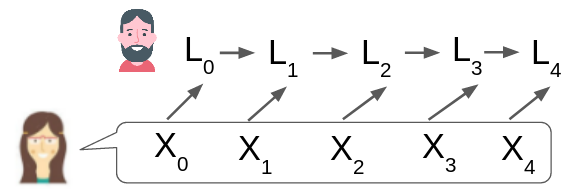
\includegraphics[width=0.45\textwidth]{figures/markov-condition.png}
	\caption{Illustration of (\ref{eq:listener-markov}). As the utterance unfolds, the listener maintains a memory state. After receiving word $X_t$, the listener computes their new memory state $L_t$ based on the previous memory state $L_{t-1}$ and the new word $X_t$.}\label{fig:listener-markov}
\end{figure}





There are no assumptions about the memory architecture and the nature of its computations.
We only make a basic assumption about the flow of information (Figure~\ref{fig:listener-markov}):
At a given point in time, the listener's memory state $L_t$ is determined by the last word $X_t$, and the prior memory state $L_{t-1}$.
As a consequence, $L_t$ contains no information about the process beyond what is contained in the last word observed $X_{t-1}$ and in the memory state before that word was observed $L_{t-1}$.
This is formalized as a statement about conditional probabilities:
	\begin{equation}\label{eq:listener-markov}
p(L_1| (X_{t})_t, L_0)   = p((X_{t})_t| L_0, X_1)
%p((X_{t})_t| L_0, L_1, X_1)   = p((X_{t})_t| L_0, X_1)
	\end{equation}
This says that $L_1$ contains no information about the utterances beyond what is contained in $L_0$ and $X_1$.	
As a consequence, the listener has no knowledge of the speaker's state beyond the information provided in their prior communication.
This is a simplification, as the listener could obtain information about the speaker from other sources, such as their common environment (weather, ...).
For the study of memory in sentence processing, this seems fair. Discuss this more.

%
%First, we assume that the listener's internal state cannot depend on the future beyond its dependency on the past.
%Formally: 
%\begin{equation}\label{eq:listener-markov-1}
%L_t \bot X_{>t} | X_{\leq t}
%\end{equation}
%This means that the listener has no access to the speaker's state beyond what the speaker has already uttered.
%
%Second, we assume that $L_t$ contains no information about the past beyond what is contained in $X_{t-1}$ and $L_{t-1}$:
%\begin{equation}\label{eq:listener-markov-2}
%L_t \bot X_{<t} | X_{t-1}, L_{t-1}
%\end{equation}
%This means that any information about the past in $L_t$ has to be contained in $L_{t-1}$ -- formalizing the idea that a listener can only remember aspects of the past by keeping them in memory, and that memories of the past cannot `spontaneously' form later in the future.

%The listener can trade off memory and future surprisal:
%A listener who chooses to store less memory will exerience higher surprisal in the future.
%A listener can achieve minimal surprisal -- that is, the lowest average surprisal that any model could achieve by predicting the future from the past -- if and only if $L_t$ contains all predictive information about the future that is contained in the past.

%We now describe the memory-surprisal tradeoff. will describe this tradeoff, and show that listener memory is linked to locality in a way similar to speaker memory.
%Consider a listener who uses $J$ bits of memory on average.
%What can we say about the listener's surprisal?




\paragraph{Conditional Mutual Information}

We will use the concept of \emph{conditional mutual information} (Figure~\ref{fig:it-surprisal-intuition}).
%For two random variables $X, Y$, the mutual information $I[X,Y]$ is the reduction in entropy about $X$ by knowing $Y$:
%\begin{equation}
%	I[X,Y] := H[X] - H[X|Y]
%\end{equation}
%For three random variables $X, Y, Z$, the mutual information between $X$ and $Y$, conditional on $Z$, is this entropy reduction when $Z$ is already known:
%\begin{equation}
%I[X,Y|Z] := H[X|Z] - H[X|Z,Y]
%\end{equation}
%We will use the specific form where $X$ and $Y$ are observations $X_0$, $X_t$ of the process $(X_t)_{t \in \mathbb{Z}}$, and $Z$ is a block of intervening observations $X_1, \dots, X_{t-1}$:
\begin{equation}
%	I[X_t, X_0 | X_1, \dots, X_{t-1}] := H[X_t| X_1, \dots, X_{t-1}] - H[X_t| X_0, X_1, \dots, X_{t-1}]
	I_t := H[X_t| X_1, \dots, X_{t-1}] - H[X_t| X_0, X_1, \dots, X_{t-1}]
\end{equation}
This is equal to the reduction in uncertainty about the $t$-th observation when knowing the $0$-th observation, in addition to the block of intervening observations.
That is, we measure the amount of statistical dependency of observations that are $t$ steps apart, controlling for any information that is redundant with intervening observations.
This quantifies how much information needs to be carried across $t$ timesteps without any possibility for `guessing' it from intervening observations.



\begin{figure*}
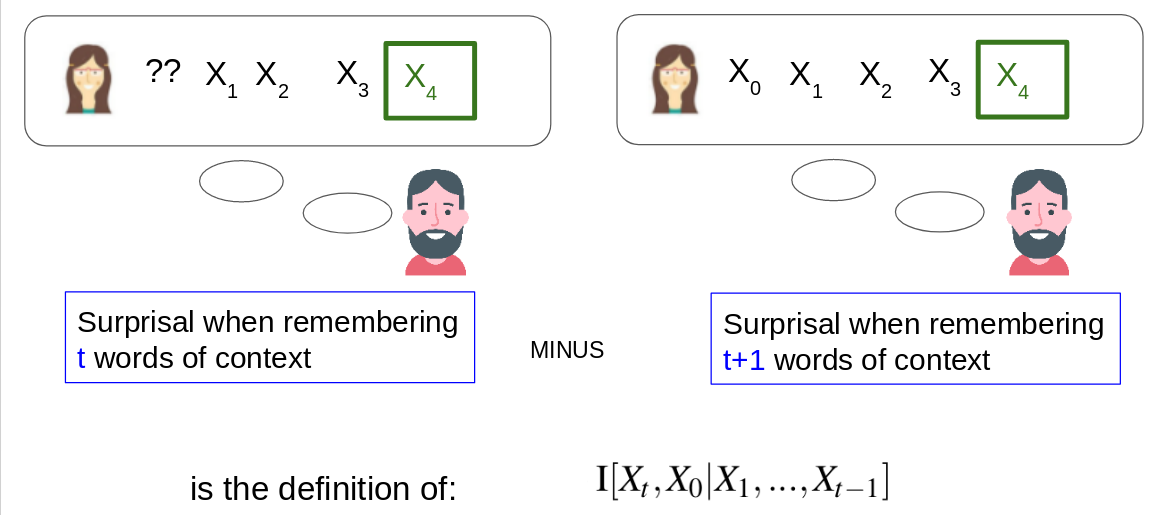
\includegraphics[width=0.9\textwidth]{figures/listener-it.png}
	\caption{(TODO adapt to format) Intuitive explanation of $I_t$}\label{fig:it-surprisal-intuition}
\end{figure*}





We return to the information and memory curves in Figure~\ref{fig:basic}.
In the graph of $t \cdot I_t$, we look for the first $T$ such that the area under the curve to the left of $T$ has size $\geq J$.
This is illustrated in Figure~\ref{fig:listener-tradeoff-decay} (right).
Then let $\epsilon$ be the area under the curve of $I_t$ to the right of $T$ (Figure~\ref{fig:listener-tradeoff-decay}, left).
We can prove that such a listener must incur surprisal at least $\epsilon$ greater than a listener with perfect memory.
As before, we write $$I_t := I[X_t, X_0 | X_{1\dots t-1}]$$
Then


\begin{thm}\label{prop:suboptimal}
	Let $T$ be any positive integer ($T \in \{1, 2, 3, ...\}$), and consider a listener using at most
	\begin{equation}\label{eq:memory}
		\sum_{t=1}^T t I_t
	\end{equation}
bits of memory on average.
Then this listener will incur surprisal at least
	$$H[X_t|X_{<t}] + \sum_{t > T} I_t$$
	on average.
\end{thm}
The proof is given in the appendix (REF).

%An intuitive (non-rigorous) argument goes as follows:
%For each bit of information that is held in memory, we count the number of timesteps from when it is first entered into memory to when it is forgotten.


\begin{figure*}
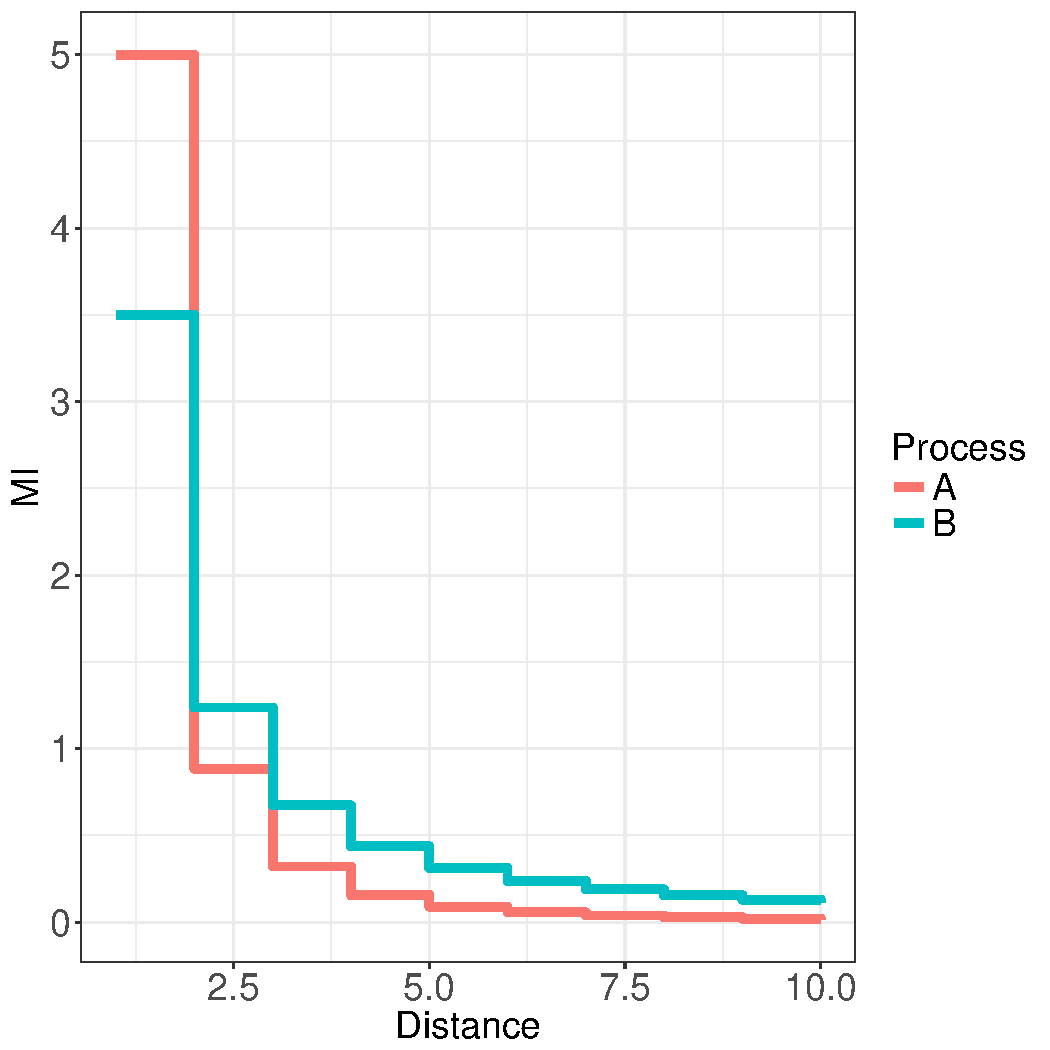
\includegraphics[width=0.45\textwidth]{toy/decay.pdf}
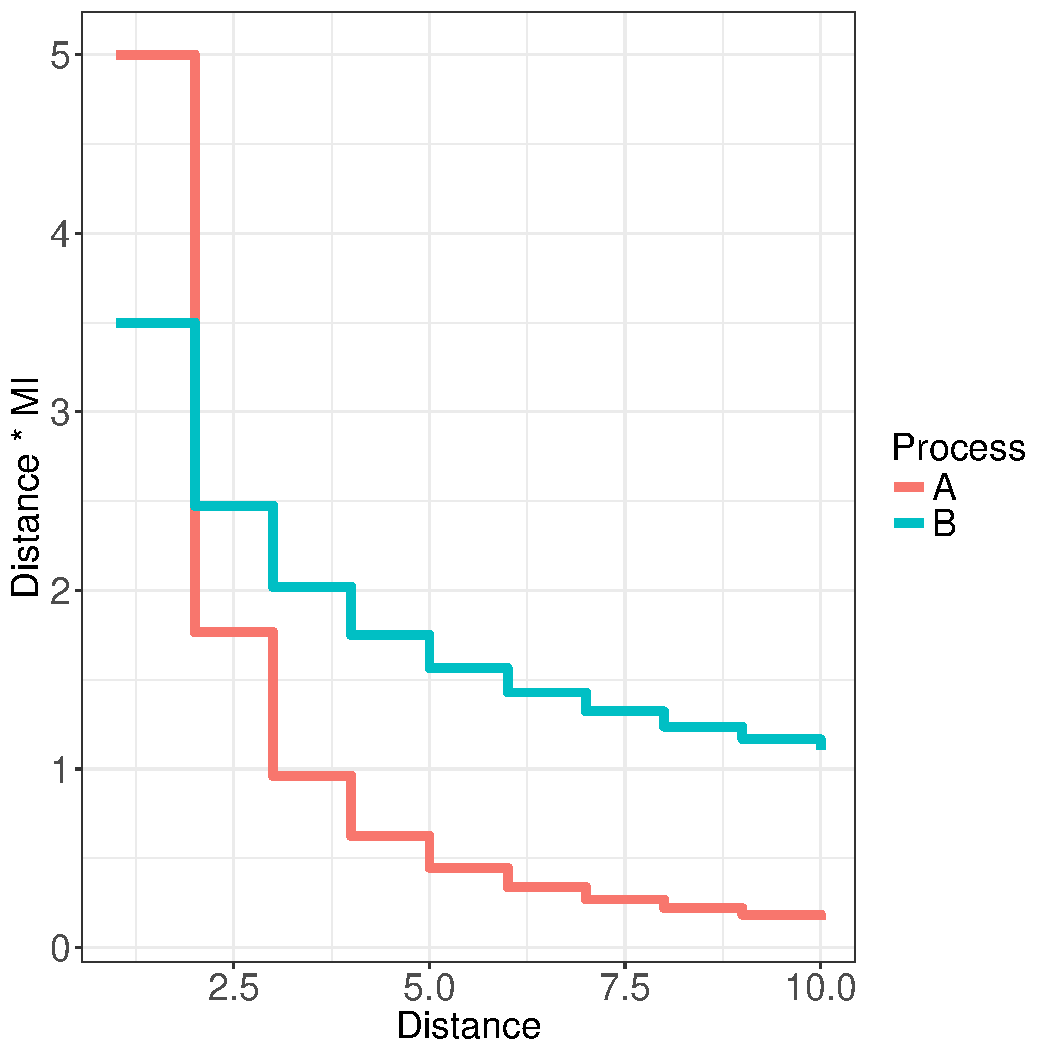
\includegraphics[width=0.45\textwidth]{toy/memory.pdf}
%
	\caption{Left: $I_t$ as a function of $t$, for two different processes. $I_t$ decays faster for the red process: Predictive information about the present observation is concentrated more strongly in the recent past. Left: $t \cdot I_t$ as a function of $t$ for the same processes. }\label{fig:basic}
\end{figure*}


\begin{figure}
	\begin{center}
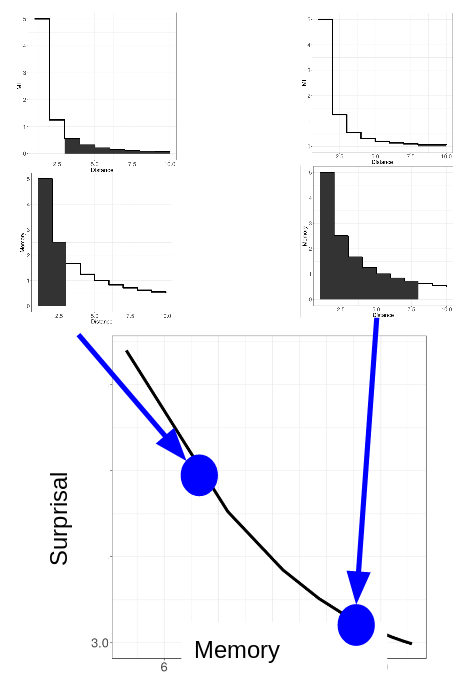
\includegraphics[width=0.45\textwidth]{figures/interpolate-curve.png}
\end{center}
	\caption{Estimating memory-surprisal tradeoff using the Theorem: We trace out the memory and surprisal values for all $T=1, 2, ...$, and linearly interpolate the curve.}\label{fig:interpolate}
\end{figure}







The proposition gives us a lower bound on the listener's memory-surprisal curve: Taking all pairs of memory $\sum_{t=1}^T t I_t$ and surprisal $H[X_t|X_{<t}] + \sum_{t > T} I_t$.
Then interplate linearly (justify this in appendix).
We obtain a curve in memry-surprisal plane, which is a lower bound on the memory demands of any listener at a given surprisal level.
We visualize this for the two processes from Figure~\ref{fig:basic} in Figure~\ref{fig:listener-tradeoff}.

\begin{figure}
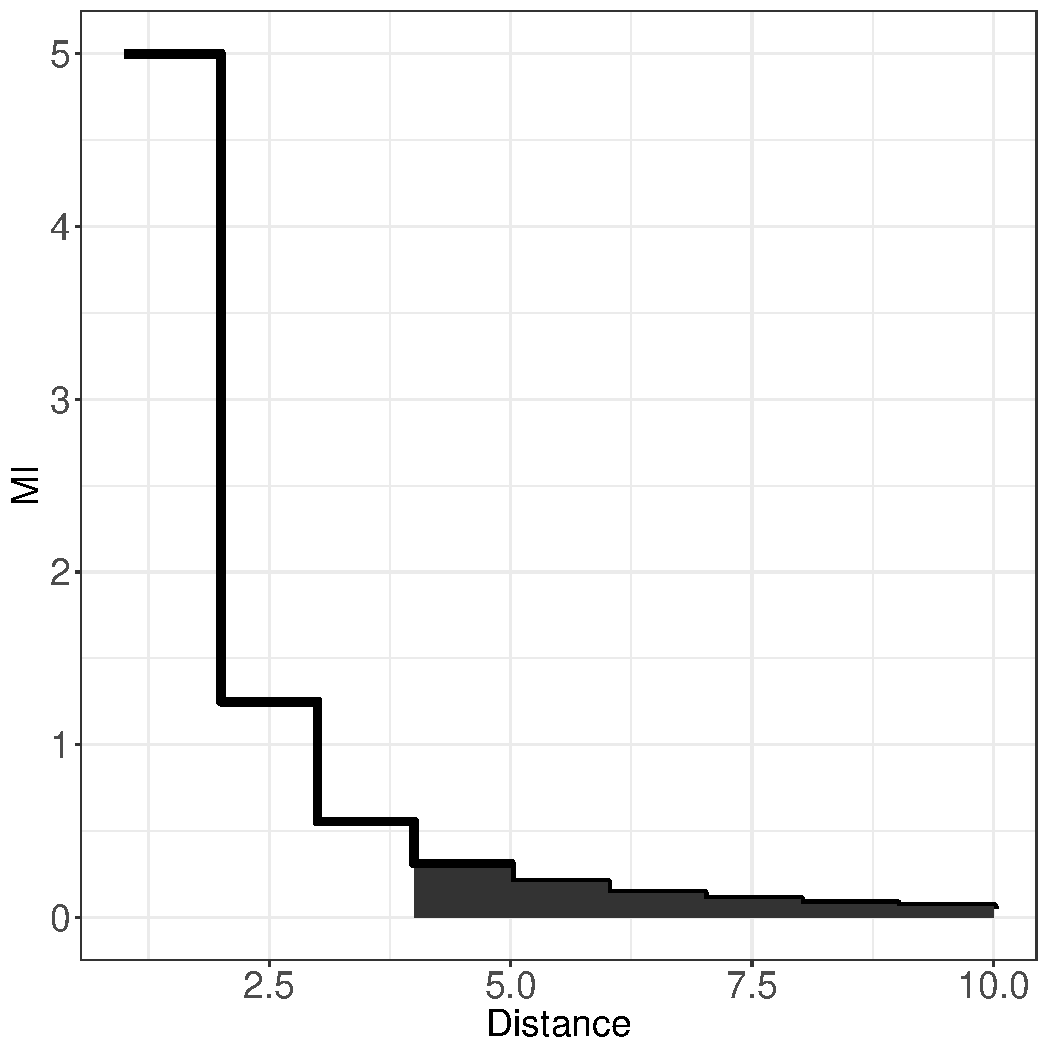
\includegraphics[width=0.45\textwidth]{toy/add-surp.pdf}
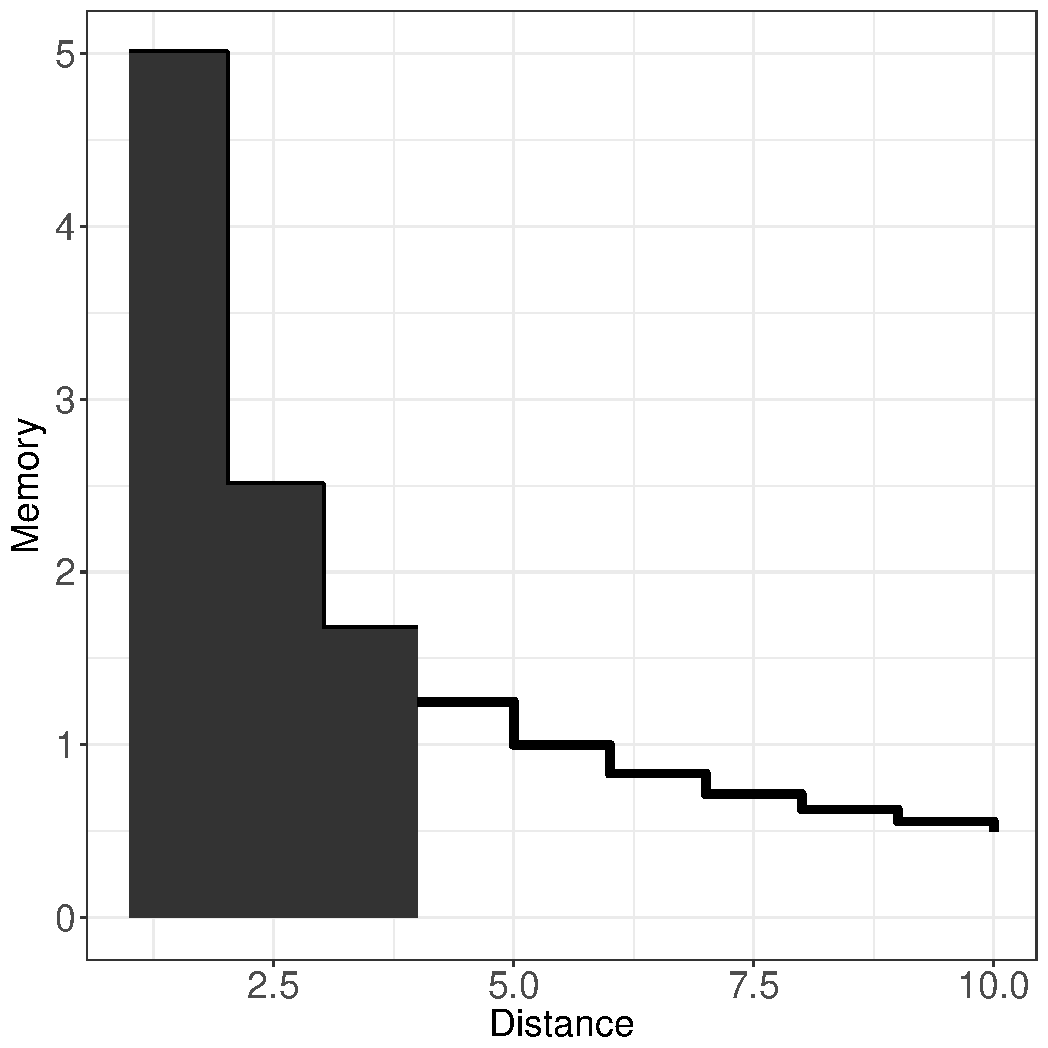
\includegraphics[width=0.45\textwidth]{toy/lower-mem.pdf}
	\caption{Illustration for Proposition~\ref{prop:suboptimal}. Listeners can trade off memory and surprisal: A listener only investing memory of the amount given by the black area on the right will incur at least the black area on the left in additional surprisal. In the given example, $T=4$. By varying $T$, the two areas describe the listener's memory-surprisal tradeoff curve.}\label{fig:listener-tradeoff-decay}
\end{figure}




\begin{figure}
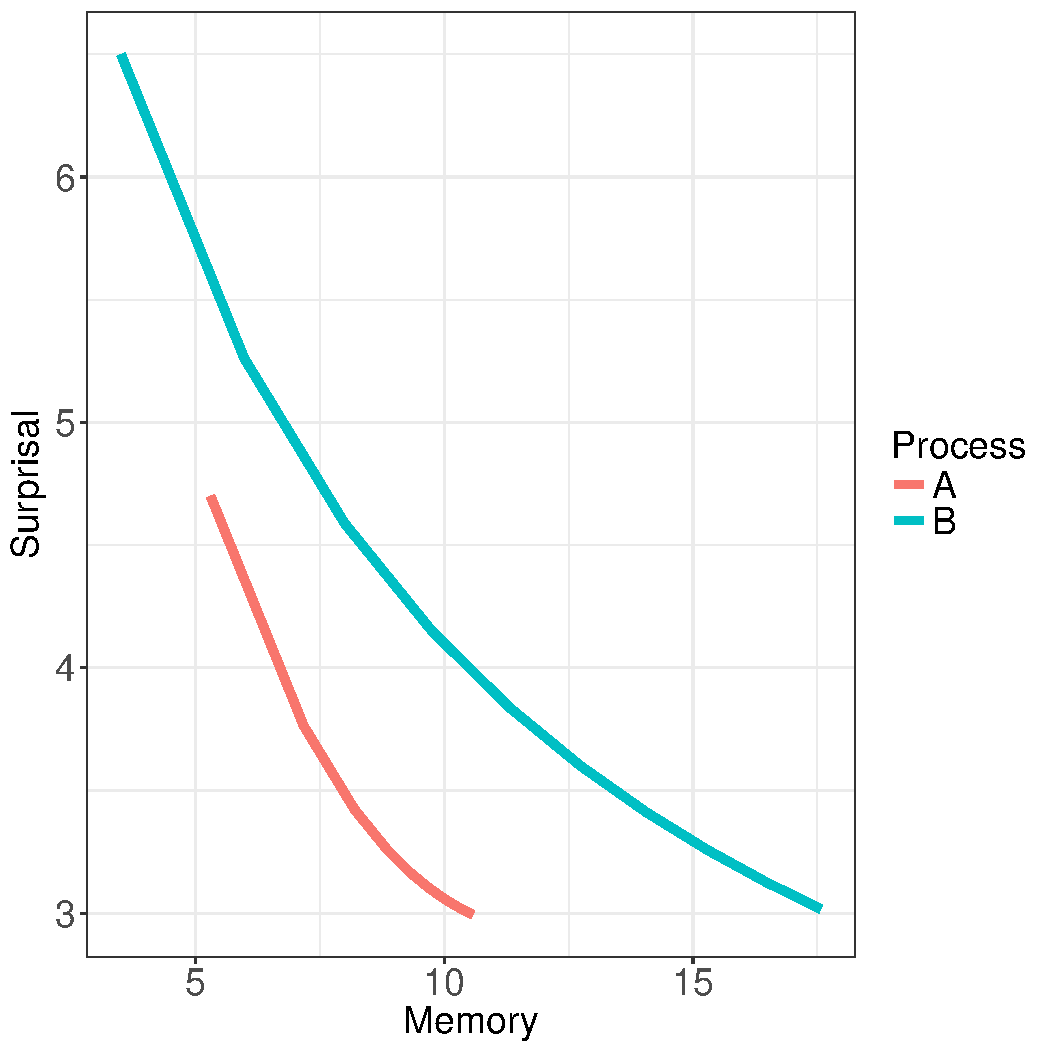
\includegraphics[width=0.45\textwidth]{toy/listener-tradeoff.pdf}
	\caption{Listener's memory-surprisal tradeoff for the two processes in Figure~\ref{fig:basic}. Recall that the red process had a faster decay of conditional mutual information. Correspondingly, this figure shows that a listener can achieve lower surprisal at the same level of memory load.}\label{fig:listener-tradeoff}
\end{figure}



\begin{figure}
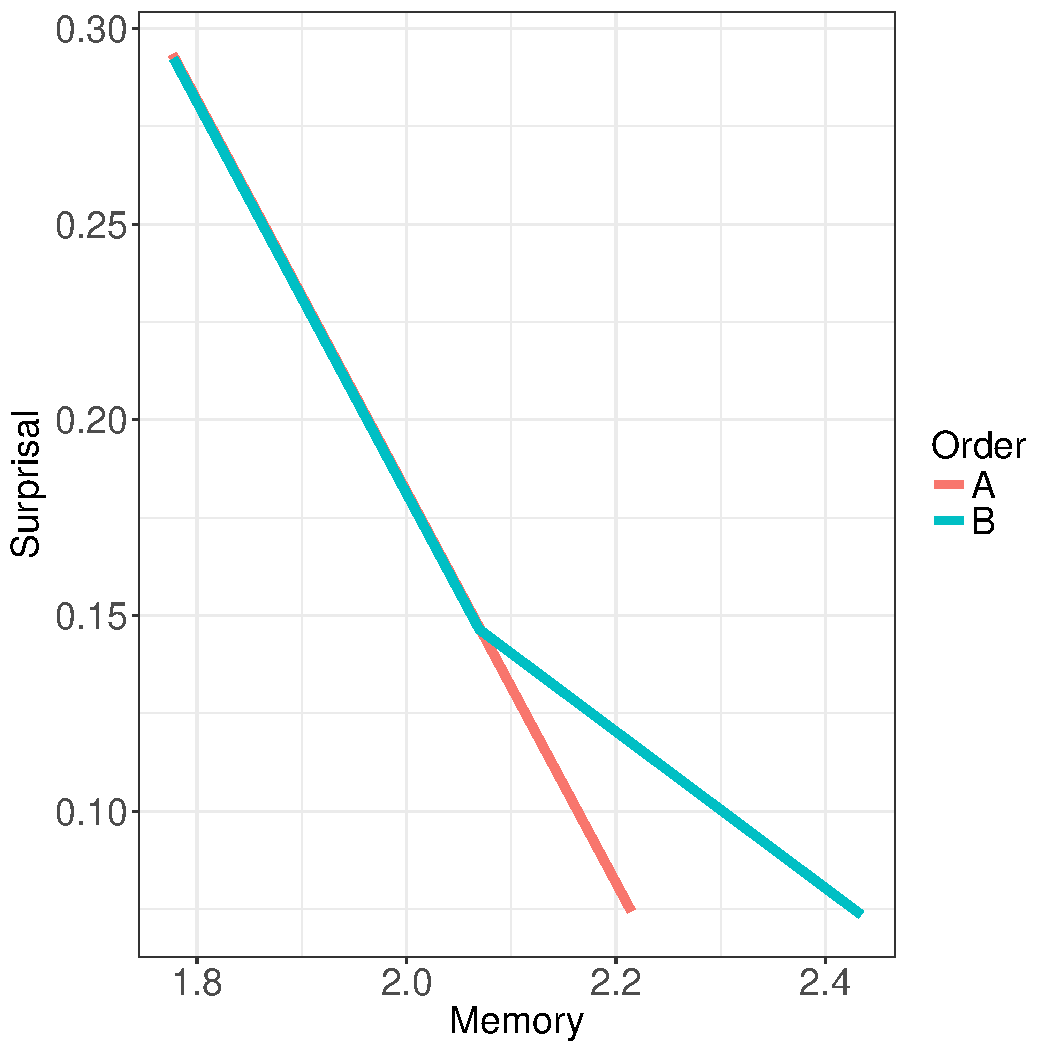
\includegraphics[width=0.45\textwidth]{toy/toy-mem-surp.pdf}
	\caption{Tradeoff between listener memory and surprisal, for the two versions of the artificial language from \cite{fedzechkina-human-2017}. Language A requires less memory at the same level of surprisal.}\label{fig:toy-listener-tradeoff}
\end{figure}








%that the model does not have an `absolute clock' built into it.


Our result is entirely information-theoretic and applies to \emph{any} physical encoding of the past, entirely independent of the implementation of the model. % and the mechanisms by which it computes predictions.
In particular, while the relation to psycholinguistic and psychological models of how memory works will be interesting to explore, our result applies to any such model.
Memory representations do not have to be rational or optimal for this bound to hold:
It provides a \emph{lower bound} on the amount of information that needs to be stored -- other memory representations will always need to store at least as much information.


\paragraph{Information Locality}


Due to the factor $t$ inside each term of the sum, carrying the same amount of information over longer distances requires more memory -- that is, modeling long statistical dependencies is more costly in terms of memory than modeling shorter ones.
This formalizes a general, assumption-free, link between memory and locality in language production.
In Section~\ref{sec:listener}, we will extend this analysis to listeners performing incremental prediction.
%incremental prediction.




%We will write $I_t$ as an abbreviation for $\operatorname{I}[X_t, X_0 | X_1, ..., X_{t-1}]$.
The proposition implies that memory is decreased if $I_t$ decreases quickly as $t \rightarrow \infty$ -- that is, if the contributions of long-term dependencies in the process are small.
In particular, memory load can only be finite if $I_t$ decreases fast enough for the infinite sum to converge to a finite value.
%This confirms the intuition that finiteness of memory entails that the contribution of long-term 


%\paragraph{Discussion}
%We have treated the process $(X_t)_t$ as a discrete-time process whose time steps correspond to words, but this is immaterial to the analysis.
%The analysis is not even restricted to discrete timesteps: We can replace thes sum in Proposition~\ref{prop:suboptimal} with an integral to get a continuous-time version.



We illustrate Proposition~\ref{prop:lower-bound} in Figure~\ref{fig:basic}.
We consider two processes A and B, where $I_t := 5t^{-1.5}$ for $A$ and $I_t := 3.5 t^{-2.5}$ for $B$.
The curves of $I_t$, as a function of the distance $t$, are shown in Figure~\ref{fig:basic} (left).
In both cases, $I_t$ converges to zero as $t$ grows to infinity. 
However, $I_t$ decays more quickly for Process A (red).
This means that predictive information about an observation is concentrated more strongly in the recent past.
In Figure~\ref{fig:basic} (right), we show $t\cdot I_t$ as a function of $t$.
Note that the area under the curve is equal to (\ref{eq:memory-bound}).
This area is smaller for the red process, as $I_t$ decays more quickly there.  


\section{Experiment 1: Memory and Dependency Length}




We illustrate the linguistic predictions of Proposition \ref{prop:lower-bound} by reanalyzing the data from \cite{fedzechkina-human-2017}.
This is a miniature artificial language study that showed a bias for Dependency Length Minimization in production in artificial language learning.
Due to the controlled setting, it is possible to exactly compute the speaker's memory as given in~(\ref{eq:memory-bound}).


As ~(\ref{eq:memory-bound}) is invariant under reversal of the language, we only consider the head-final version of her artificial language.
The language has consistent head-final order, and uses case marking on objects.
The relevant production targets are transitive sentences where one of the two arguments is much longer than the other, due to the presence of a PP modifier, as shown in Table~\ref{tab:artificial}.
The language has variable order of subjects and objects; for the production targets, the B versions produce much longer dependencies than the A versions.
Dependency Length Minimization thus predicts that speakers are more likely to use the A versions.
\cite{fedzechkina-human-2017} confirmed this experimentally.


\begin{table}
	\textbf{A Orders: Short Dependencies}

		\begin{tabular}{ccc}
			Object & Subject & Verb \\
			\fbox{\begin{tabular}{llllll}
				\fbox{\begin{tabular}{llll} Adjective &Noun &Postposition\end{tabular}} & Noun-Case
					\end{tabular}} & \fbox{\begin{tabular}{l}Noun\end{tabular}} & \fbox{\begin{tabular}{l}Verb\end{tabular}}  \\
		\end{tabular}
\\
		\begin{tabular}{ccc}
			Subject & Object & Verb \\
			\fbox{\begin{tabular}{llllll}
				\fbox{\begin{tabular}{llll} Adjective &Noun &Postposition\end{tabular}} & Noun
					\end{tabular}} & \fbox{\begin{tabular}{l}Noun-Case\end{tabular}} & Verb \\
		\end{tabular}
\\
\\

	\textbf{B Orders: Long Dependencies}


		\begin{tabular}{ccc}
			Subject & Object & Verb \\
			 \fbox{\begin{tabular}{l}Noun\end{tabular}} &  \fbox{\begin{tabular}{llllll}
				\fbox{\begin{tabular}{llll} Adjective &Noun &Postposition\end{tabular}} & Noun-Case
		\end{tabular}}  &  \fbox{\begin{tabular}{l}Verb\end{tabular}}  \\
		\end{tabular}
\\
		\begin{tabular}{ccc}
			Object & Subject & Verb \\
			\fbox{\begin{tabular}{l}Noun-Case\end{tabular}} & \fbox{\begin{tabular}{llllll}
				\fbox{\begin{tabular}{llll} Adjective &Noun &Postposition\end{tabular}} & Noun
		\end{tabular}} & Verb \\
		\end{tabular}

			\caption{Production targets in the artificial mini language from \cite{fedzechkina-human-2017}. The language has head-final order, with free variation between SO and OS orders. When one of the arguments is much longer than the other, placing the longer one first (`A' orders) shortens syntactic dependencies, compared to `B' orders.}\label{tab:artificial}

\end{table}

In this section, we show that our bound on speaker memory makes the same prediction, without reference to syntactic structure or specific memory architectures. 

We constructed one language consisting of the A versions, and one language consisting of the B versions.
Following the experimental setup of \cite{fedzechkina-human-2017}, we assigned equal probability to the two possible configurations per language, and used a separate set of nouns (inanimate nouns) for the embedded noun in the long phrase.

We interpreted each of the two languages as a stationary processes, extending infinitely in both directions, by concatenating independent samples drawn from the language.
			We computed (\ref{eq:memory-bound}) from a chain of 1000 independently sampled sentences, for each of the two versions of the toy language.
			Figure~\ref{fig:toy-mis} (left) shows the curve of the conditional mutual information $I_t$ as a function of the distance $t$.
			The curves differ at $t=2$ and $t=5$: 
			About 0.073 nats of predictive information that are at distance $t=2$ in the A orders are moved to $t=5$ in the B orders.
%			In this sense, A orders have greater information locality than the B orders.
			%What is responsible for this difference?
			The source of the difference lies in predicting the presence and absence of a case marker on the second argument -- i.e., whether to anticipate a subject or object.
			In the A orders, considering the last two words is sufficient to make this decision.
			In the B orders, it is necessary to consider the word before the long second constituent, which is five words in the past.

			The total amounts of predictive information -- corresponding to the area under the curve -- are the same, indicating that both languages are equally predictable.
			However, we will see that the memory demands are different:
			Figure~\ref{fig:toy-mis} (right) shows $t\cdot I_t$ as a function of $t$.
			As $I_t$ decays faster in A orders, the total area under the curve now differs between A and B, and is larger in B.
			%This area corresponds to the lower bound in (\ref{eq:memory-bound}), and is 2.21 nats in A orders, and 2.43 nats in B orders.

%While (\ref{eq:memory-bound}) is a general lower bound, it can be proven that this bound is actually tight in the case of this specific example.\footnote{This can be shown by computing the causal states and then showing that the crypticity is zero, both of which is tractable in the case of this small-scale artificial language.}
%That is, a speaker who optimally allocates memory resources will spend 2.21 nats in A orders, and 2.43 nats in B orders.


In Figure~\ref{fig:toy-listener-tradeoff}, we show the resulting curve for the two versions of the artificial language from \cite{fedzechkina-human-2017}.
%In this language, speaker memory coincides with the memory demand of a listener who performs optimally in incremental prediction.
The curve shows that, at any desired level of surprisal, Order A requires at most as much memory as Order B.
For reaching optimal surprisal, Order A requires strictly less memory.
Thus, in this case, the listener's surprisal-memory tradeoff is optimized by the orders predicted by Dependency Length Minimization.

It is important to stress that, even though we computed this value by considering the number of words impacting predictions at a given point in time, this bound holds independently of the actual implementation and architecture of memory and predictions.




\begin{figure*}
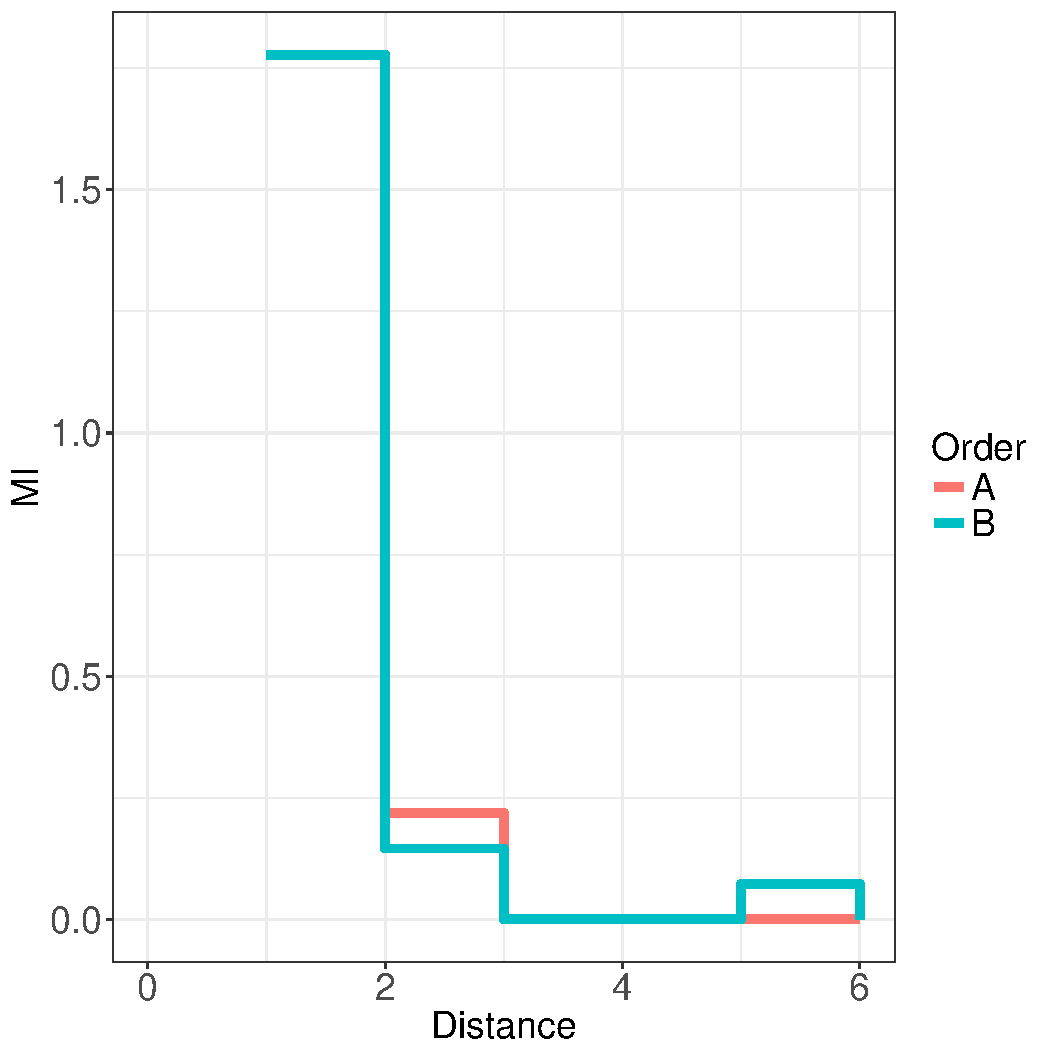
\includegraphics[width=0.45\textwidth]{toy/toy-mis.pdf}
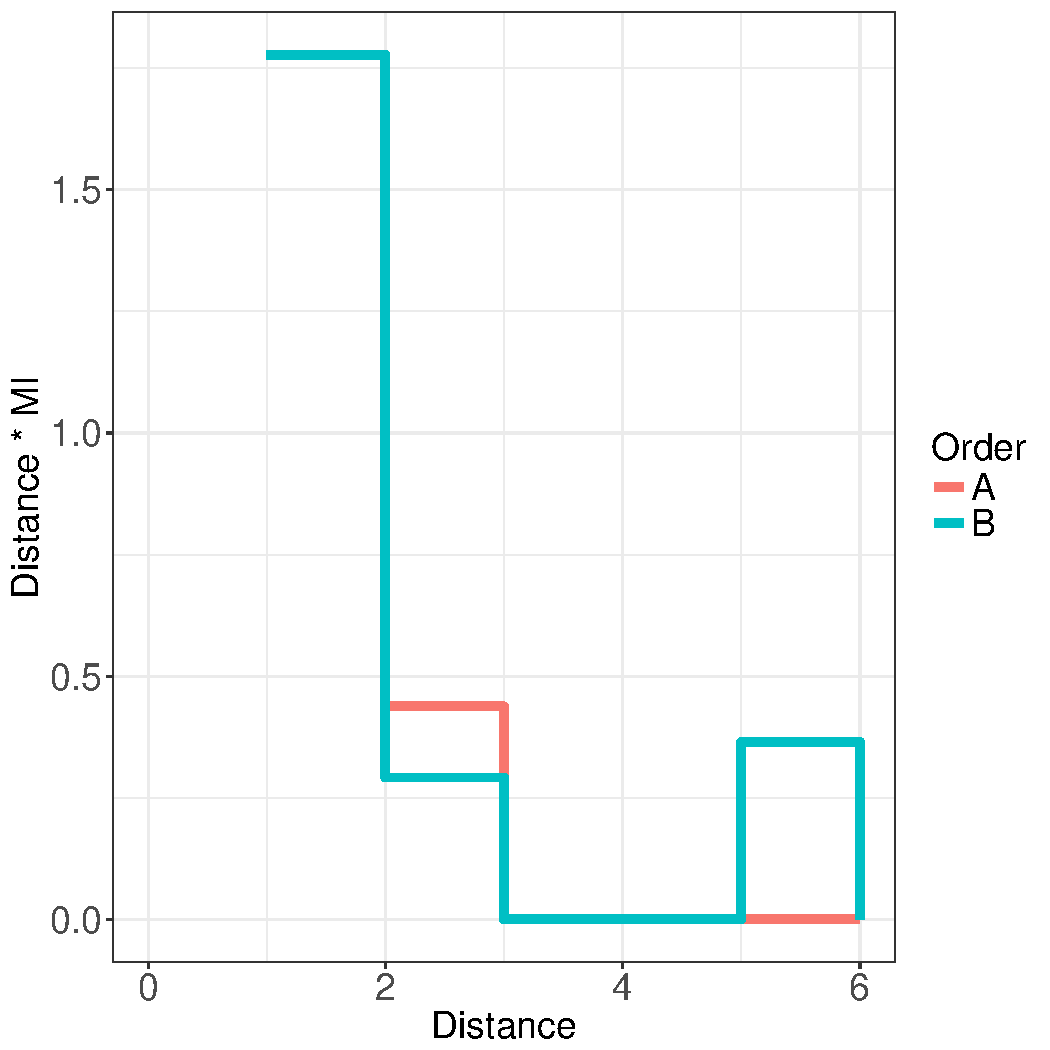
\includegraphics[width=0.45\textwidth]{toy/toy-t-mis.pdf}
%
	\caption{Left: Decay of Conditional Mutual Information, as a function of the distance $t$, for the two versions in the artificial language. The areas under the two curves are identical, corresponding to the fact that both orders are equally predictable. However, mutual Information decays faster in Order A.\ \ \ Right: $t I_t$, as a function of $t$. The area under the B curve is larger, corresponding to larger memory demand for this order.}\label{fig:toy-mis}
\end{figure*}
%Both languages have the same overall entropy rate, but they differ in the distribution of predictive information.
%
%plot of $I_t$
%
%The areas under the curves are identical.
%
%good version
%
%%CONTEXT LENGTH 0   2.06856758681  9997.93143241   0.0
%%CONTEXT LENGTH 1   0.29195106479  1.77661652202   1.77661652202
%%CONTEXT LENGTH 2   0.0729865489103  0.21896451588   2.21454555377
%%CONTEXT LENGTH 3   0.0729865489103  0.0   2.21454555377
%%CONTEXT LENGTH 4   0.0729865489103  0.0   2.21454555377
%%CONTEXT LENGTH 5   0.0729865489103  0.0   2.21454555377
%%CONTEXT LENGTH 6   0.0729865489103  0.0   2.21454555377
%
%bad version
%
%%CONTEXT LENGTH 0   2.06937301571  9997.93062698   0.0
%%CONTEXT LENGTH 1   0.291673373027  1.77769964269   1.77769964269
%%CONTEXT LENGTH 2   0.145830550934  0.145842822093   2.06938528687
%%CONTEXT LENGTH 3   0.145830550934  0.0   2.06938528687
%%CONTEXT LENGTH 4   0.145830550934  0.0   2.06938528687
%%CONTEXT LENGTH 5   0.0729152754672  0.0729152754672   2.43396166421
%%CONTEXT LENGTH 6   0.0729152754672  0.0   2.43396166421
%%CONTEXT LENGTH 7   0.0729152754672  0.0   2.43396166421
%%
%
%
%
%%
%%grammar:
%%
%%S $\rightarrow$ Obj Subj V (1/2) | Subj Obj V (1/2)
%%
%%Obj $\rightarrow$ NP di
%%
%%Subj $\rightarrow$ NP
%%
%%NP $\rightarrow$ N (3/4) | PP NP (1/8) | Adj NP (1/8)
%%
%%PP $\rightarrow$ NP P
%%
%
%

\begin{figure}
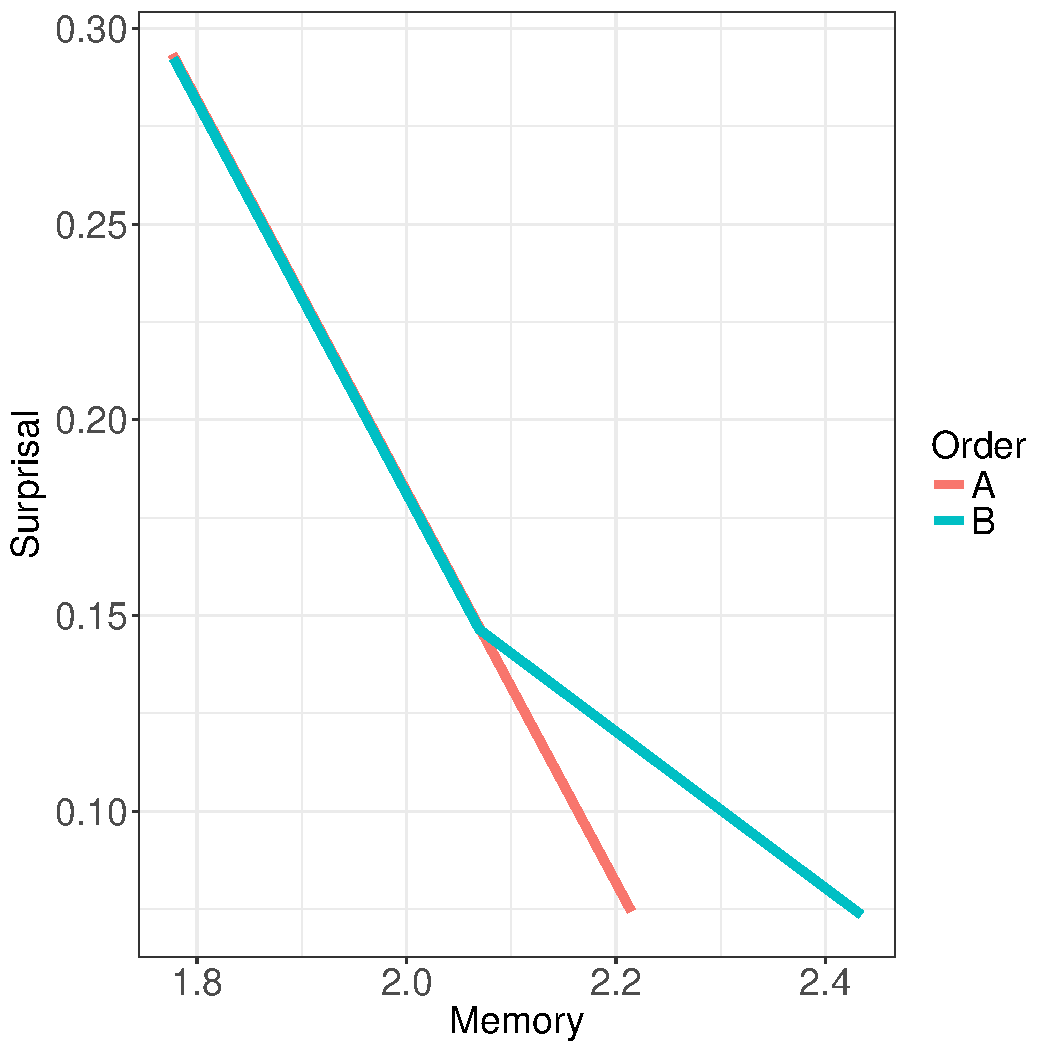
\includegraphics[width=0.45\textwidth]{toy/toy-mem-surp.pdf}
	\caption{Tradeoff between listener memory and surprisal, for the two versions of the artificial language from \cite{fedzechkina-human-2017}. Language A requires less memory at the same level of surprisal.}\label{fig:toy-listener-tradeoff}
\end{figure}





\paragraph{Center Embeddings}

\cite{miller-finitary-1963} attributed the unacceptability of multiple center-embedding to memory limitations.


%\cite{gibson-linguistic-1998}

%first center-embeddings, POS level model

%Later work found evidence that cross-serial dependencies are less taxing.


%now cross-serial: POS level model things are the same. But lexical level, assume PMI and dependencies. Then listener's tradeoff is better for cross-serial dependencies

\paragraph{Other Psycholinguistic Predictions}

% RF: the fact that you would get locality effects given medium WM capacity, but not very high or very low WM capacity, as Bruno Nicenboim found. And maybe some speaker-listener asymmetries. 

\paragraph{Speakers}

% RF: what matters for the speaker is not I[X_t, X_0 | X_1, …, X_{t-1}], but I[X_t, X_0 | X_1, …, X_{t-1}, G] where G is some representation of the speaker’s goal (like in the van Dijk paper). This changes the interpretation of the mutual information. For the listener, it’s just redundancy. For the speaker, it’s redundancy *conditional on the goal*—which you could interpret as something like conceptual relatedness of linguistic elements. Then the speaker’s pressure is to keep conceptually related things close. 


\section{Large-Scale Evidence that natural language optimize Memory-Surprisal Tradeoff}

We now investigate whether word orders as found in natural language optimize the two memory-surprisal tradeoffs.
We compare the memory-surprisal tradeoffs of 52 actual languages to those of counterfactual reorderings.
We cannot just compare to random orderings of individual syntactic trees, as such languages would not have word order regularities.
Therefore, we compare to counterfactual word order grammars.

\begin{figure}
\centering
\begin{dependency}[theme = simple]
   \begin{deptext}[column sep=1em]
	   I \&	   wrote \& risāla \& li \& sadīq  \\
   \end{deptext}
	%   \deproot{3}{ROOT}
   \depedge{1}{2}{obj}
	%   \depedge[edge start x offset=-6pt]{2}{5}{ATT}
   \depedge{1}{4}{obl}
   \depedge{4}{3}{case}
   %\depedge[arc angle=50]{7}{6}{ATT}
\end{dependency}
	\caption{TODO Dependencies example}\label{fig:dependency}
\end{figure}



\subsection{Data}
We draw on corpora annotated with syntactic structures.
The Universal Dependencies project has compiled dependency corpora for several dozen languages~\citep{nivre-universal-2017}.

\paragraph{Dependency Grammar}
In dependency corpora, sentences are annotated with \emph{dependency trees} (Figure~\ref{fig:dependency}).
These are directed trees describing the grammatical relations among words. For example, the arcs labeled ``obj'' represent that the noun in question is the \emph{direct object} if the verb, rather than e.g. the subject or an indirect object.
A dependency arc is drawn from a \emph{head} (e.g. TODO in Figure TODO) to a \emph{dependent} (e.g. TODO).
Dependency trees can be defined in terms of many different syntactic theories \cite{corbett1993heads}.
Although there are some differences in how different formalisms would draw trees for certain sentences, there is broad enough agreement about dependency trees that it has been possible to develop large-scale dependency-annotated corpora of text from dozens of languages \cite{nivre2017universal}.

\paragraph{Corpora}
We considered all languages for which there are Universal Dependencies 2.2 treebanks with a total of at least 500 sentences of training data.
We excluded data from historical languages.\footnote{Ancient Greek, Coptic, Gothic, Latin, Old Church Slavonic, Old French.}
This resulted in 52 languages.

For each of these languages, we pooled all available corpora in one dataset.
We excluded corpora that primarily contain text created by non-native speakers.
Universal Dependencies corpora have a predefined split into \emph{training}, \emph{held-out} (also known as \emph{development}), and \emph{test} partitions.
While larger corpora have all three partitions, smaller corpora often have only some of these partitions.
For most language, we used the predefined data split, separately pooling data from the different partitions. %We did not use the test partitions.
For some languages with little data, there is no predefined training partition, or the training partition is smaller than the other partitions.
In these cases, we redefined the split to obtain more training data:
For these languages, we pooled all the available partitions, used 100 randomly selected sentences as held-out data, and used the remainder as training data.\footnote{This affects Amharic, Armenian, Breton, Buryat, Cantonese, Faroese, Kazakh, Kurmanji, Naija, Thai, and Uyghur.}
For each language, we used the training and held-out sets for estimating the memory-surprisal tradeoff (see Section~\ref{sec:method}).
We provide the sizes of the resulting datasets in Table~\ref{tab:corpora}.



\subsection{Counterfactual Ordering Grammars}
We define ordering grammars, small models of the rules by which languages order syntactic structures into sentences.
Our formalism of ordering grammars adapts the method of \cite{gildea-optimizing-2007, gildea-grammars-2010, gildea-human-2015} to the setting of dependency corpora.

Universal Dependencies defines 37 universal syntactic relations that are used to label dependency arcs across all corpora.
These relations encode cross-linguistically meaningful relations such as subjects, objects, and adjectival modifiers.
We define ordering grammars by assigning a parameter $a_\tau \in [-1,1]$ to every one of these 37 universal syntactic relations.
Relations sometimes have language-specific subtypes; we do not distinguish these subtypes.

In our model, this parameter defines how dependents are ordered relative to their head:
Given a head and a set of dependents, we order each dependents by the parameter $a_\tau$ assigned to the syntactic relation linking it to the head.
Dependents with negative weights are placed to the left of the head; dependents with positive weights are placed to the right.

Ordering grammars describe languages that have consistent word order:
For instance, the subject is consistently ordered before or after the verb, depending on whether the parameter for the verb-subject dependency is positive or negative.

We define baseline grammars by randomly sampling the parameters $a_\tau$.
Such baseline grammars define languages that have consistent word order, but do not exhibit any systematic correlations between the orderings of different dependents.



\paragraph{Discussion}
In actual languages, the ordering of words is largely determined by the syntactic relations (CITE).
However, certain kinds of rules cannot be modeled by our word order grammars, such as rules sensitive to the category of the dependent (e.g., differences between nominal and pronominal objects).
Word order freedom also is not modeled.
In this sense, ordering grammars represent approximations to the kinds of ordering rules found in natural language \cite{gildea-optimizing-2007, gildea-grammars-2010, gildea-human-2015}.



\subsection{Estimating Memory-Surprisal Tradeoff}\label{sec:method}
To estimate mutual informations, we use LSTM recurrent neural networks, the basis of the state of the art in modeling natural language (CITE) and predicting the surprisal effect on reading times~\citep{frank-insensitivity-2011, goodkind-predictive-2018}.
%We model language on the level of individual word forms.
We provide data from alternative estimation methods in the SI.


%\paragraph{Data}



%Given a sequence of input words $w_1, ..., w_n \in V$, the model 
%%
%\textbf{TODO I'm describing this in a lot of detail. Alternatively, we can say this is a standard NLP method and refer to the NLP literature for the definition.}
%The first component of such a model is an \emph{embedding matrix} $W_{emb} \in \mathbb{R}^{|V| \times d_{emb}}$, where the \emph{vocabulary} $\mathcal{V}$ is a set, containing the words that occur in the corpus, and $d_{emb} \in \mathbb{N}$ is a fixed parameter.
%This matrix assigns a $d_{emb}$-dimensional vector to each word occurring in the corpus.
%The second component is an LSTM cell $f_{LSTM}$, a nonlinear transformation mapping an \emph{input} vector $x_{i} \in \mathbb{R}^{d_{emb}}$ a \emph{hidden state} $h_i \in \mathbb{R}^{d_{LSTM}}$ and a \emph{cell state} $c_i \in \mathbb{R}^{d_{LSTM}}$ to a new pair of hidden state and cell states $h_{i+1}, c_{i+1} \in \mathbb{R}^{d_{LSTM}}$.
%The LSTM cell $f_{LSTM}$ is parameterized by a matrix of numerical parameters $W_{LSTM}$.
%
%%Such networks estimate the probability of a word in context as follows.
%Given a sequence of input words $w_1, ..., w_n \in V$, the model first retrieves fixed-dimensionality vector representations $x_1, ..., x_n$, where $x_i$ is the row of $W_{emb}$ corresponding to the word $w_i$.
%It then computes a sequence of hidden and cell states by the following recurrent computation:
%\begin{align*}
%	h_1, c_1 &:= 0 \\
%	h_2, c_2 &:= f_{LSTM}(x_1, h_1, c_1) \\
%	\dots \\
%	h_{n+1}, c_{n+1} &:= f_{LSTM}(x_n, h_n, c_n) \\
%\end{align*}
%The vector $h_i$ encodes the result of reading the words $w_1, ..., w_{i-1}$.
%We will write $LSTM(w_1, ..., w_{i-1})$ for $h_i$.
%
%The third component of the recurrent language model is the matrix $W_{output} \in \mathbb{R}^{|V| \times d_{LSTM}}$.
%We obtain per-word predictions of the next word by computing
%\begin{align*}
%	s_i := W_{output} h_i \in \mathbb{R}^{|V|} \\
%	p_i := \operatorname{softmax}(s_i)\in \mathbb{R}^{|V|} 
%\end{align*}
%where the softmax transformation normalizes vectors into probability distributions as follows
%\begin{equation}
%	\operatorname{softmax}(x)_i := \frac{\exp(x_i)}{\sum_{j=1}^{|V|} \exp(x_j)}
%\end{equation}
%Finally, the probability of the word $w_n$ in the context $w_1, ..., w_{n-1}$ is computed as
%\begin{equation}
%	p_\theta(w_n|w_1...w_{n-1}) := \frac{\exp((p_n)_{w_n})}{\sum_{w \in V} \exp(x_w)}
%\end{equation}
%and thus the surprisal is estimated as
%\begin{equation}
%- \log	p_\theta(w_n|w_1...w_{n-1}) := -\log \frac{\exp((p_n)_{w_n})}{\sum_{w \in V} \exp(x_w)}
%\end{equation}
%We discuss the choice of the numerical parameters in the next section.
%

\paragraph{Model and Parameter Estimation}
We use a recurrent neural network with Long-Short-Term Memory cells~\citep{hochreiter-long-1997} (CITE for Neural LM).
This architecture takes as input a sequence $x_1 ... x_N$ of words, and at each time step $t=1, ..., N$, calculates a probability distribution over the next word $w_{t}$ given preceding words $w_1 ... w_{t-1}$: $p(w_t|w_1...w_{t-1})$.

The network is parameterized by a vector $\theta$ of weights determining how the activations of neurons propagate through the network~\citep{hochreiter-long-1997}.
Given a corpus, the numeral parameters of the LSTM are chosen so as to minimize the average surprisal across the training corpus.
%We can think of the LSTM parameters as forming one large vector $\theta$.
At the beginning of training, the parameters $\theta$ are randomly initialized.

The training corpus is chopped into word sequences $w_1 ... w_T$ of length $T$ ($T = 20$ in our experiments).
If $\theta_n$ consists of the LSTM parameters after $n$ training steps, we randomly select a word sequence $w_1 ... w_T$ from the training corpus, and use the LSTM using the current parameter setting $\theta_n$ to compute the per-word surprisals.
We then update the parameter vector:
\begin{equation}\label{eq:train}
	\theta_{n+1} := \theta_n + \alpha \partial_\theta \left(\sum_{i=1}^T \log p_\theta(w_i|w_1...w_{i-1})\right)
\end{equation}
where $\alpha \in \mathbb{R}_+$ is the \emph{learning rate}.
When calculating the parameter update, we use three standard methods of regularization that have been shown to improve neural language modeling: dropout~\citep{srivastava-dropout:-2014}, word dropout, and word noising~\citep{xie2017data}.
In this process, the word sequences are sampled without replacement.
Once all sequences have been processed, we start another pass through the training data.
Before each pass through the training data, the order of sentences of the training data is shuffled, and the corpus is again chopped into sequences of length $T$.

After each pass through the training data, the average surprisal at the current parameter setting $\theta_n$ is evaluated on the held-out partition.
We terminate training once this held-out  surprisal does not improve over the one computed after the previous pass any more.



%\paragraph{Regularization}
%Dropout, Word dropout, Word noising
%Any statistical estimation problem faces the 
%The quality of neural network models is further improved by regularization, improving generalization to the full data distribution.
%In the case of neural networks, the most successful regularization methods typically take the form of random modifications to the input and internal activations when computing the gradients in the training updates~(\ref{eq:train}).
%First, we apply \emph{dropout} both to the input vectors $x_i$ and to the output vectos $h_i$, randomly setting individual elements to zero with rate $p_{embedding} \in [0,1]$.
%Second, we apply \emph{word dropout}, randomly zeroing out entire input vectors $x_i$ at rate $p_{word}$.

\paragraph{Choice of Hyperparameters}

The LSTM model has a set of numerical \emph{hyper-parameters} that need to be specified before parameter estimation, namely the dimensionalities of the embeddings $d_{emb}$, the dimensionality of the hidden states $d_{LSTM}$, and the number of LSTM layers $d_{layer}$, the learning rate $\alpha$, and the regularization parameters (dropout rate $p_{embedding}$, word dropout rate $p_{word}$, word noising rate $p_{noising}$).
We choose these parameters so as to minimize the average surprisal on the held-out partition resulting at the end of parameter estimation.

For each corpus, we used Bayesian optimization using the Expected Improvement acquisition function \citep{snoek-practical-2012} to find a good setting of the hyperparameters.
We optimized the hyperparameters to minimize average surprisal on languages generated from random word order grammars.
This biases the hyperparameters towards modeling counterfactual grammars better, biasing them \emph{against} our hypothesis.

For computational efficiency, neural language models can only process a bounded number of distinct words in a single language.
For each corpus, we limited the number of distinct processed words to the $N=10,000$ most common words in the training corpus, a common choice for neural language models (CITE).
Following (CITE), we represented other words by their part-of-speech tags as annotated in the corpora.
This applied to 37 languages, affecting an average of 11~\% of words in this languages.
We believe that this modeling limitation does not affect our results for the following reasons.
First, this affects the same words in real and counterfactually ordered sentences.
Second, all excluded words are extremely infrequent in the available data, occurring less than 10 times (except for Czech and Russian, the languages for which we have by far the largest datasets).
Many of the excluded words occur only once in the dataset (78 \% on average across the affected languages).
This means that any model would only be able to extract very limited information about these words from the available training data, likely \emph{less} than what is provided by the part-of-speech tag.
Third, traditional N-gram models, which do not have this limitation, provide results in qualitative agreement with the neural network-based estimates (see SI).

%Given a corpus, we estimate a language model by training the LSTM on a training partition to maximize the data likelihood, and stopping training once the data likelihood on a held-out partition drops.
%The hyperparameters (number of hidden units, learning rate, etc.) are chosen so as to maximize the likelihood of the held-out partition.
%This procedure helps prevent overfitting the model to the training data, and ensure that it generalizes to unseen data. 



\paragraph{Estimating the Memory-Surprisal Tradeoff Curve}



The quantity $\operatorname{I}[X_t, X_0 | X_1, ..., X_{t-1}]$ in~(\ref{eq:memory-bound}) is equal to the difference 
\begin{equation}
H[X_t|X_1, ..., X_{t-1}] - H[X_t|X_0, X_1, ..., X_{t-1}]
\end{equation}
For each word in the held-out partition, we compute the difference
\begin{equation}
	-\log P_\theta[X_t | X_0, X_1, ..., X_{t-1}] - P_\theta[X_t | X_1, ..., X_{t-1}]
\end{equation}
and take the average over these.
We cut $T$ off at 20, as this is the length of the sequences processed by the model.

We then used linear interpolation to interpolate the surprisal value for memory values in between these values. (TODO make a figure).
This is justified theoretically (TODO maybe discuss when introducing the theorem).

We estimate the unigram entropy $H[X_0]$ by averaging over all models.

%
%\subsection{Discussion: Alternative Models}
%In view of the NLP literature, the following are the main other options that exist for estimating mutual information and probabilities in sequences:
%
%A traditional model uses n-gram models. A challenge of n-gram models is that they do not express any morphosyntactic generalizations. Furthermore, standard n-gram models do not express any generalizations about pairs of words that are not adjacent -- e.g., encoding a generalization about morphological agreement between two words is hard for such a model to capture if the two words are not always adjacent. Both the small scale of available corpora in many languages and free word order in many languages with rich morphology thus seem to make such models unattractive.
%We evaluate our hypothesis using n-gram models in SI Section X, confirming the conclusions obtained from neural models.
%
%A second option is to construct a statistical grammar, such as PCFG.
%The challenge is to encode statistical morphosyntactic generalizations, and to decide which independence assumptions to put into the model.
%One can either decide on a language-specific basis which generalizations to put in (laborious and might introduce bias), or choose a general model family that is rich enough to learn generalizations.
%The second option will make this a machine learning model that, for our purposes, does not seem to be superior to a recurrent neural network.
%



%\subsection{Data}
%\subsection{Setup}
%The recurrent neural network architecture has a range of adjustable parameters such as the number of neurons.
%For each language, we used Bayesian optimization using the Expected Improvement acquisition function (CITE) \citep{snoek-practical-2012} to find a good setting of the hyperparameters, taking average surprisal on random grammars as the objective.
%This biases the hyperparameters towards favoring counterfactual grammars.

%\subsection{Setup}

For each language, we collected data from the actual orderings and from several random grammars.
We collect multiple samples for the actual orderings to control for variation due to the random initialization of the neural network.
For each of the random grammars, we collect one sample.
Data is collected according to a precision-based stopping criterion described in Section (REF).
%We collected data from the actual and random orderings in proportion one to two.
%The stopping criterion will be described below.

%Due to the randomness both in the sequence of training examples and the random initialization of the network weights, the results of the parameter estimation procedure will vary when run multiple times, especially on smaller datasets.
%Informally, due to the finiteness of the dataset, multiple parameter settings are compatible with the available training data.
%Consequently, memory-surprisal tradeoffs estimated on held-out sets will also show some variation.
%Therefore, we collect multiple samples for the actual orderings to control for variation due to the random initialization of the neural network.


%We chose these thresholds based on preliminary simulations which had suggested that these widths were achievable at acceptable computational cost.

%- at least 30 samples from both baseline and real
%
%- for the language-level tradeoff curve, either the fraction is zero or the bootstrapped CI has width $\leq 0.2$.



%
%(1) is bigram MI always greater in real languages?
%
%(2) is the tradeoff curve always lower than for deterministic simple grammar? for deterministic complex grammars? for stochastic simple/complex grammars?


\subsection{Statistics}

We now describe how we compared memory-surprisal tradeoffs between real and baseline languages.

%For each sample, we estim
%For each language, we viewed surprisal as a function of memory.
%We used linear interpolation to obtain surprisal values for all levels of memory.

We want to test whether languages' surprisal-memory tradeoffs better than those of most baseline languages.
%We view surprisal as a function of memory load, so that the curve is defined on all of $\mathbb{R}_+$.
We compare real and baseline languages by evaluating which languages result in lower surprisal at the same level of memory.
We now describe the statistics we use to quantifying the difference between real and baseline languages.
We do everything in a frequentist framework (null hypothesis testing \& confidence intervals), as we can do exact tests and confidence intervals without parametric assumptions.
Maybe we can explain how the tests \& CIs also have reasonable Bayesian interpretations (for the specific methods used here, rejection of the null should guarantee that the posterior of the null hypothesis is small under a wide range of priors.).

\paragraph{Confidence Interval for Medians}
We use a (nonparametric and nonasymptotic) confidence interval for the median surprisal at each memory value, using the binomial test.
We consider the medians over all runs for the real language, and over all baselines grammars.

% yStudyTradeoff_Bootstrap_Parallel_OnlyWordForms_BoundedVocab_BinomialTest_Single_MedianCI.py


\paragraph{CI for Median Difference}
We create (nonparametric and nonasymptotic) confidence interval for the difference between real and baseline median surprisals at each memory value.

% yStudyTradeoff_Bootstrap_Parallel_OnlyWordForms_BoundedVocab_BinomialTest_Single_MedianDiffCI.py


\paragraph{Pointwise Significance Test}
For each memory value $\mu$, we do a nonparametric and nonasymptotic significance hypothesis test against the null hypothesis that at least half of the baseline grammars have lower surprisal than the actual language (Figure~\ref{fig:nhst-pointwise}).
Formally, let $W_-(\mu)$ be the proportion of baseline languages that have strictly lower surprisal than the real language at memory level $\mu$.
We take the real language to be represented by the \emph{sample median}.
For each level $\mu$ of memory, we consider the null hypothesis that
\begin{equation}
	W_-(\mu) \leq 0.5
\end{equation}
%In reality, we do not observe the curve of the real language exactly, but as noisy samples from our computational estimator.
We use the Binomial Test.

%This statistic also should have a reasonable Bayesian interpretation:
% E.g., if the random samples are unimodal, and we do inference over only the median (location family), 



\begin{figure}
	\begin{center}
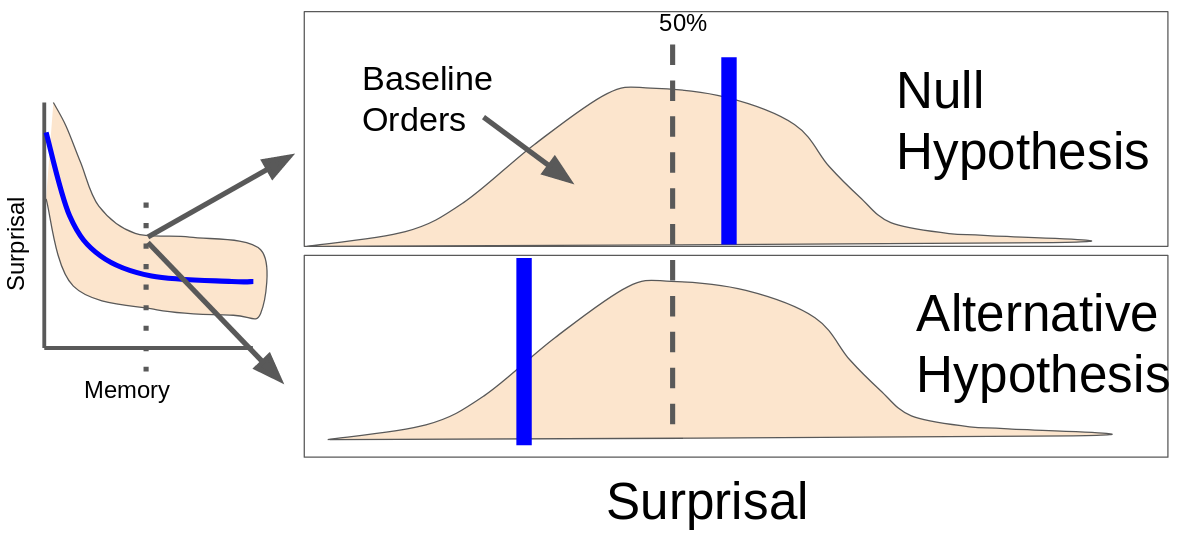
\includegraphics[width=0.45\textwidth]{figures/nhst.png}
\end{center}
	\caption{Illustration for the pointwise null-hypothesis significance test. At a given level of memory, we test against the null hypothesis that at least half of the baseline orders provide lower surprisal than the real language.}\label{fig:nhst-pointwise}
\end{figure}






%For each memory value $\mu$, we do a significance test (nonparametric and nonasymptotic).
%\begin{equation}
%	W_+(\mu) \geq W_-(\mu)
%\end{equation}
%We use the empirical median for the real language.

% yStudyTradeoff_Bootstrap_Parallel_OnlyWordForms_BoundedVocab_BinomialTest_Single.py

%We take the REAL values to be estimated exactly by their medians.



\paragraph{Pointwise Quantile Estimate}
%CI for quantile: % yStudyTradeoff_Bootstrap_Parallel_OnlyWordForms_BoundedVocab_BinomialTest_Single_UnimodalBoundOnQuantile_BothDirections.py

\begin{figure}
	\begin{center}
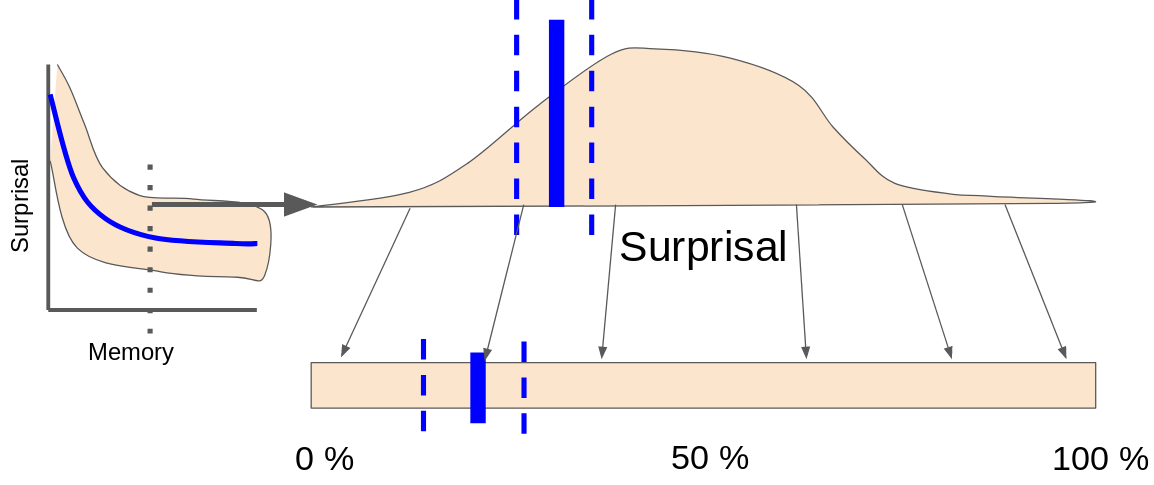
\includegraphics[width=0.45\textwidth]{figures/quantile.png}
\end{center}
	\caption{Illustration for the quantile estimate. At each level of memory, we provide an estimate of the percentage of baseline languages that have lower surprisal than the real language.}\label{fig:quantile-pointwise}
\end{figure}


For each level of memory, we estimate what percentage of baseline languages have lower surprisal than the real language.
This is described in Figure~\ref{fig:quantile-pointwise}.

We derive a confidence interval under the assumption that the distribution of baseline languages is unimodal.

We derive a CI for the quantile, under the assumption that the baseline distribution is unimodal. We take the REAL values to be estimated exactly by their medians.

We want to create a CI at each Memory value for the quantile.

Let $n_+$ be the better baseline samples, $n_-$ the worse ones.

Let $\theta$ the best baseline sample that is worse than the real median.

We want to get a confidence bound $q$ on $P(X < x_{real})$.

Let $p := P(N_+ \leq n_+ | N_+ + N_-; q)$.
Then output $(0, q)$ as a level $p$ CI for the parameter $P(X < x_{real})$.

We minimize $q$ subject to $p < 0.05$.

Once we have $q$, we can make it a bit better under the assumption that the baseline distribution is unimodal.

This CI is exact in the sense that it does not involve asymptotic approximations or parametric assumptions, but it is extremely conservative.

Also the following does not assume unimodality, and ends up getting about the same intervals
% yStudyTradeoff_Bootstrap_Parallel_OnlyWordForms_BoundedVocab_BinomialTest_Single_UnimodalBoundOnQuantile_BothDirections_NoAssumption.py




\paragraph{Global Quantile Estimate}


\begin{figure}
	\begin{center}
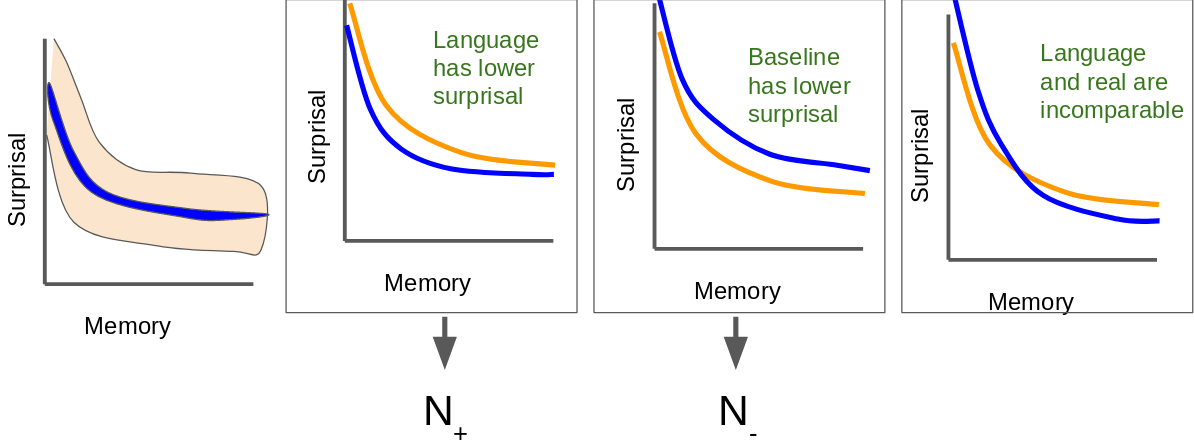
\includegraphics[width=0.45\textwidth]{figures/quantile-global.png}
\end{center}
	\caption{Illustration for the global quantile estimate. For each sample for the real language, we compare the memory-surprisal curve to all baselines.}\label{fig:quantile-global}
\end{figure}



For each sample $x$ from real orderings, we look at the proportions $N_+(x)$ of samples from the baseline languages that are more optimal than $x$ throughout the entire range where both curves are defined, and the proportion $N_-(x)$ of baseline samples that are consistently less optimal.

%We consider the null hypothesis that, on average, not more baseline languages are consistently less optimal than are consistently more optimal than the real orderings:
%\begin{equation}
%	\E_{x \sim P_1}[W_+(x)] \geq \E_{x \sim P_1}[W_-(x)]
%\end{equation}

We estimate the quotient
\begin{equation}\label{eq:g}
	G :=	\frac{\E_{x \sim P_1}[W_+(x)]}{\E_{x \sim P_1}[W_+(x) + W_-(x)]}
\end{equation}
where $P_1$ is the distribution over values obtained for real orderings.
We use a bootstrapped confidence interval for $\E[G]$ for quantifying the degree of optimization.
For bootstrapping, we separately resample samples from the real language and from the baseline grammars.

Unlike the other statistics, this one provides a global measure of the degree of optimization of the real language.
Due to the use of bootstrapping, the confidence intervals are not exact.


%- bootstrapping
%- subsampling
%- permutation test / rank test ??
%



\subsection{Number of Samples}
Training neural language models is computationally costly.
Therefore, we used a precision-based stopping criterion to adaptively choose a sample size for each language.
Precision-based stopping criteria offer a way to adaptively choose sample size without biasing results (CITE).

For each language, we first collected 10 data points for real orderings and 10 data points for baseline orderings.
We continued obtaining new data points until the CI for $G$ had width $\leq 0.15$, or there were 100 samples from $P_1$ and 300 samples from $P_2$.
Up to the end, we chose the next sample to be from $P_0$ with probability 2/3, and $P_1$ otherwise.\footnote{Due to a scripting error, a much higher number of samples was generated for Erzya.}

This procedure was parallelized on several machines.
In the case where the stopping criterion was reached for a language while several machines were still computing samples for this language, we did not discard those samples.
Consequently, more samples were collected than necessary to reach the stopping criterion; however, in a way that does not bias our results towards or against our hypothesis.

%Due to parallelization of this procedure, it often produced more samples than required, when the stopping criterion .

%We chose these thresholds based on preliminary simulations which had suggested that these widths were achievable at acceptable computational cost.

%For each language, we collected at least 5 data points for real orderings and at least 10 data points for baseline orderings.
%We continued obtaining new data points until the CI for $G$ had width $\leq 0.15$, or there were 100 samples from $P_1$ and 300 samples from $P_2$.
%Up to the end, we chose the next sample to be from $P_0$ with probability 2/3, and $P_1$ otherwise.




\subsection{Results}

The numbers of samples taken per language are provided in Table~\ref{tab:samples}.

%In Figure~\ref{tab:plain-results} (TODO), we show the estimated memory-surprisal tradeoff curves for all samples.

In Figure~\ref{tab:medians}, we show the medians for real and baseline languages.

Descriptively, the real language provides better tradeoffs than the median of the baselines across languages, with four exceptions (Latvian, North Sami, Polish, Slovak).

In Figure~\ref{tab:slice-hists-real}, we show the distribution of surprisals achieved at the maximal memory value for real and random languages.

In Figure~\ref{fig:hist-real}, we show surprisals at maximum memory, after z-transforming for each individual language and then aggregating.

In Table \ref{tab:median_diffs}, we show the differences in median surprisal, as a function of memory.


In Table~\ref{tab:boot-g}, we report the bootstrap estimates and confidence intervals for G~(\ref{eq:g}).
$\E[G]$ was not estimated to be significantly above $>5$ for four languages: Latvian, North Sami, Polish, and Slovak.


In Table~\ref{tab:quantiles}, we show the quantiles.



\begin{figure}
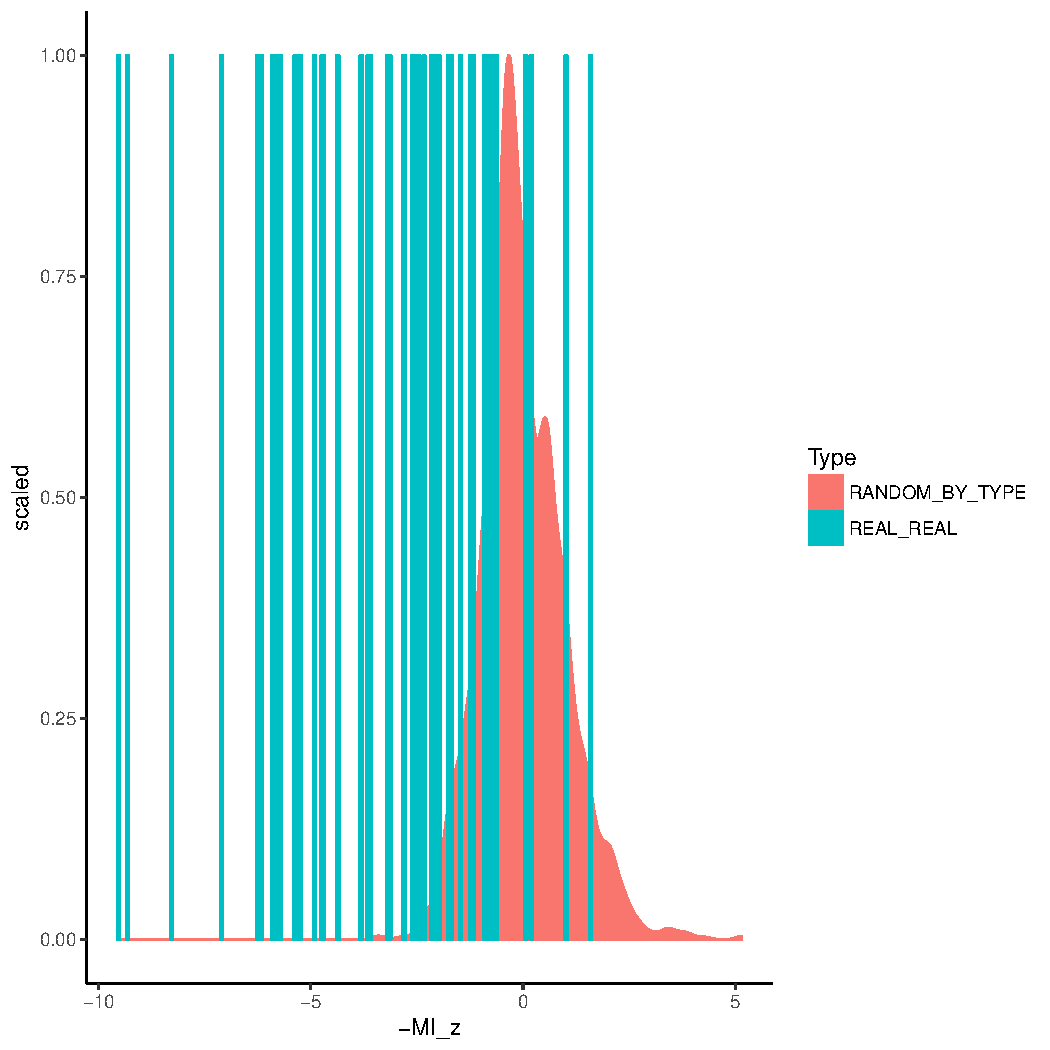
\includegraphics[width=0.95\textwidth]{neural/figures/full-REAL-listener-surprisal-memory-HIST_z_byMem_onlyWordForms_boundedVocab.pdf}
\caption{Histogram}\label{fig:hist-real}
\end{figure}


\begin{table}
\begin{longtable}{l|ll||l|llllllllllllll}
	Language & Training & Held-Out & 	Language & Training & Held-Out\\ \hline
Afrikaans  &  1,315  &  194  &  Indonesian  &  4,477  &  559  \\
Amharic  &  974  &  100  &  Italian  &  17,427  &  1,070  \\
Arabic  &  21,864  &  2,895  &  Japanese  &  7,164  &  511  \\
Armenian  &  514  &  50  &  Kazakh  &  947  &  100  \\
Bambara  &  926  &  100  &  Korean  &  27,410  &  3,016  \\
Basque  &  5,396  &  1,798  &  Kurmanji  &  634  &  100  \\
Breton  &  788  &  100  &  Latvian  &  4,124  &  989  \\
Bulgarian  &  8,907  &  1,115  &  Maltese  &  1,123  &  433  \\
Buryat  &  808  &  100  &  Naija  &  848  &  100  \\
Cantonese  &  550  &  100  &  North Sami  &  2,257  &  865  \\
Catalan  &  13,123  &  1,709  &  Norwegian  &  29,870  &  4,639  \\
Chinese  &  3,997  &  500  &  Persian  &  4,798  &  599  \\
Croatian  &  7,689  &  600  &  Polish  &  6,100  &  1,027  \\
Czech  &  102,993  &  11,311  &  Portuguese  &  17,995  &  1,770  \\
Danish  &  4,383  &  564  &  Romanian  &  8,664  &  752  \\
Dutch  &  18,310  &  1,518  &  Russian  &  52,664  &  7,163  \\
English  &  17,062  &  3,070  &  Serbian  &  2,935  &  465  \\
Erzya  &  1,450  &  100  &  Slovak  &  8,483  &  1,060  \\
Estonian  &  6,959  &  855  &  Slovenian  &  7,532  &  1,817  \\
Faroese  &  1,108  &  100  &  Spanish  &  28,492  &  3,054  \\
Finnish  &  27,198  &  3,239  &  Swedish  &  7,041  &  1,416  \\
French  &  32,347  &  3,232  &  Thai  &  900  &  100  \\
German  &  13,814  &  799  &  Turkish  &  3,685  &  975  \\
Greek  &  1,662  &  403  &  Ukrainian  &  4,506  &  577  \\
Hebrew  &  5,241  &  484  &  Urdu  &  4,043  &  552  \\
Hindi  &  13,304  &  1,659  &  Uyghur  &  1,656  &  900  \\
Hungarian  &  910  &  441  &  Vietnamese  &  1,400  &  800  \\

\end{longtable}
	\caption{Languages, with the number of training and held-out sentences available.}\label{tab:corpora}
\end{table}

\begin{table}
\begin{longtable}{l|ll||l|llllllllllllll}
	Language & Base. & Real & Language & Base. & Real \\ \hline
Afrikaans  &  13  &  10  &  Indonesian  &  11  &  11  \\
Amharic  &  137  &  10  &  Italian  &  10  &  10  \\
Arabic  &  11  &  10  &  Japanese  &  25  &  15  \\
Armenian  &  140  &  76  &  Kazakh  &  11  &  10  \\
Bambara  &  25  &  29  &  Korean  &  11  &  10  \\
Basque  &  15  &  10  &  Kurmanji  &  338  &  61  \\
Breton  &  35  &  14  &  Latvian  &  308  &  178  \\
Bulgarian  &  14  &  10  &  Maltese  &  30  &  24  \\
Buryat  &  26  &  18  &  Naija  &  214  &  10  \\
Cantonese  &  306  &  32  &  North Sami  &  335  &  194  \\
Catalan  &  11  &  10  &  Norwegian  &  12  &  10  \\
Chinese  &  21  &  10  &  Persian  &  25  &  12  \\
Croatian  &  30  &  17  &  Polish  &  309  &  35  \\
Czech  &  18  &  10  &  Portuguese  &  15  &  55  \\
Danish  &  33  &  17  &  Romanian  &  10  &  10  \\
Dutch  &  27  &  10  &  Russian  &  20  &  10  \\
English  &  13  &  11  &  Serbian  &  26  &  11  \\
Erzya  &  846  &  167  &  Slovak  &  303  &  27  \\
Estonian  &  347  &  101  &  Slovenian  &  297  &  80  \\
Faroese  &  27  &  13  &  Spanish  &  14  &  10  \\
Finnish  &  83  &  16  &  Swedish  &  31  &  14  \\
French  &  14  &  11  &  Thai  &  45  &  19  \\
German  &  19  &  13  &  Turkish  &  13  &  10  \\
Greek  &  16  &  10  &  Ukrainian  &  28  &  18  \\
Hebrew  &  11  &  10  &  Urdu  &  17  &  10  \\
Hindi  &  11  &  10  &  Uyghur  &  326  &  175  \\
Hungarian  &  220  &  109  &  Vietnamese  &  303  &  12  \\

\end{longtable}
	\caption{Samples drawn per language according to the precision-dependent stopping criterion.}\label{tab:samples}
\end{table}



\begin{table}
\begin{longtable}{l|lll||l|lllllllllllllll}
	Language & Mean & Lower & Upper & Language & Mean & Lower & Upper \\ \hline
Afrikaans  &  1.0  &  1.0  &  1.0  &  Indonesian  &  1.0  &  1.0  &  1.0  \\
Amharic  &  1.0  &  1.0  &  1.0  &  Italian  &  1.0  &  1.0  &  1.0  \\
Arabic  &  1.0  &  1.0  &  1.0  &  Japanese  &  1.0  &  1.0  &  1.0  \\
Armenian  &  0.92  &  0.87  &  0.97  &  Kazakh  &  1.0  &  1.0  &  1.0  \\
Bambara  &  1.0  &  1.0  &  1.0  &  Korean  &  1.0  &  1.0  &  1.0  \\
Basque  &  1.0  &  1.0  &  1.0  &  Kurmanji  &  0.93  &  0.88  &  0.98  \\
Breton  &  1.0  &  1.0  &  1.0  &  Latvian  &  0.49  &  0.4  &  0.57  \\
Bulgarian  &  1.0  &  1.0  &  1.0  &  Maltese  &  1.0  &  1.0  &  1.0  \\
Buryat  &  1.0  &  1.0  &  1.0  &  Naija  &  1.0  &  0.99  &  1.0  \\
Cantonese  &  0.96  &  0.86  &  1.0  &  North Sami  &  0.37  &  0.3  &  0.44  \\
Catalan  &  1.0  &  1.0  &  1.0  &  Norwegian  &  1.0  &  1.0  &  1.0  \\
Chinese  &  1.0  &  1.0  &  1.0  &  Persian  &  1.0  &  1.0  &  1.0  \\
Croatian  &  1.0  &  1.0  &  1.0  &  Polish  &  0.1  &  0.04  &  0.17  \\
Czech  &  1.0  &  1.0  &  1.0  &  Portuguese  &  1.0  &  1.0  &  1.0  \\
Danish  &  1.0  &  1.0  &  1.0  &  Romanian  &  1.0  &  1.0  &  1.0  \\
Dutch  &  1.0  &  1.0  &  1.0  &  Russian  &  1.0  &  1.0  &  1.0  \\
English  &  1.0  &  1.0  &  1.0  &  Serbian  &  1.0  &  1.0  &  1.0  \\
Erzya  &  0.99  &  0.98  &  1.0  &  Slovak  &  0.07  &  0.03  &  0.12  \\
Estonian  &  0.8  &  0.72  &  0.86  &  Slovenian  &  0.82  &  0.77  &  0.88  \\
Faroese  &  1.0  &  1.0  &  1.0  &  Spanish  &  1.0  &  1.0  &  1.0  \\
Finnish  &  1.0  &  1.0  &  1.0  &  Swedish  &  1.0  &  1.0  &  1.0  \\
French  &  1.0  &  1.0  &  1.0  &  Thai  &  1.0  &  1.0  &  1.0  \\
German  &  1.0  &  0.91  &  1.0  &  Turkish  &  1.0  &  1.0  &  1.0  \\
Greek  &  1.0  &  1.0  &  1.0  &  Ukrainian  &  1.0  &  1.0  &  1.0  \\
Hebrew  &  1.0  &  1.0  &  1.0  &  Urdu  &  1.0  &  1.0  &  1.0  \\
Hindi  &  1.0  &  1.0  &  1.0  &  Uyghur  &  0.65  &  0.57  &  0.73  \\
Hungarian  &  0.87  &  0.8  &  0.93  &  Vietnamese  &  1.0  &  0.98  &  1.0  \\

\end{longtable}
	\caption{Bootstrapped estimates for $G$.}\label{tab:boot-g}
\end{table}



\begin{table}
\begin{longtable}{ccccccccccccccclll}
Afrikaans & Amharic & Arabic & Armenian
 \\ 
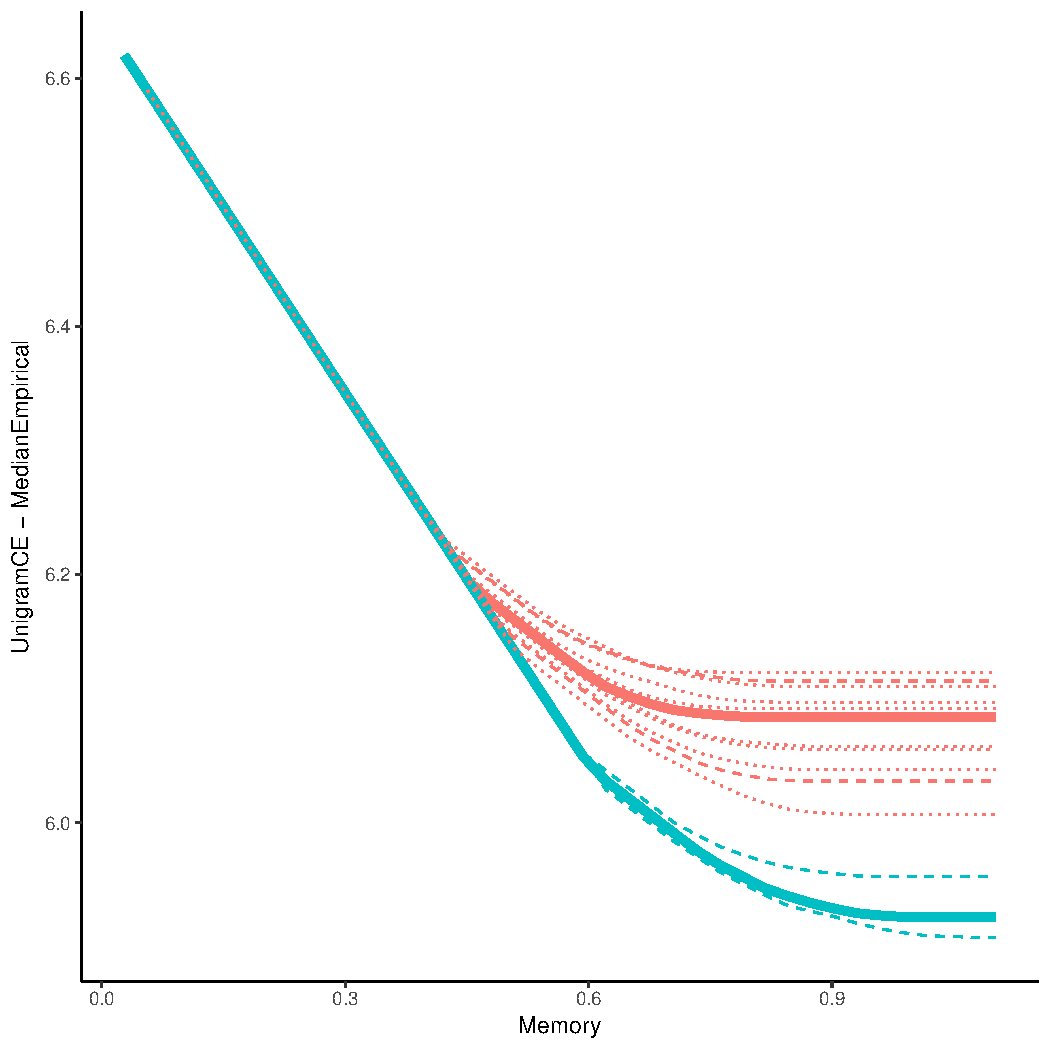
\includegraphics[width=0.25\textwidth]{neural/figures/Afrikaans-listener-surprisal-memory-MEDIANS_QUANTILES_onlyWordForms_boundedVocab_REAL.pdf} & 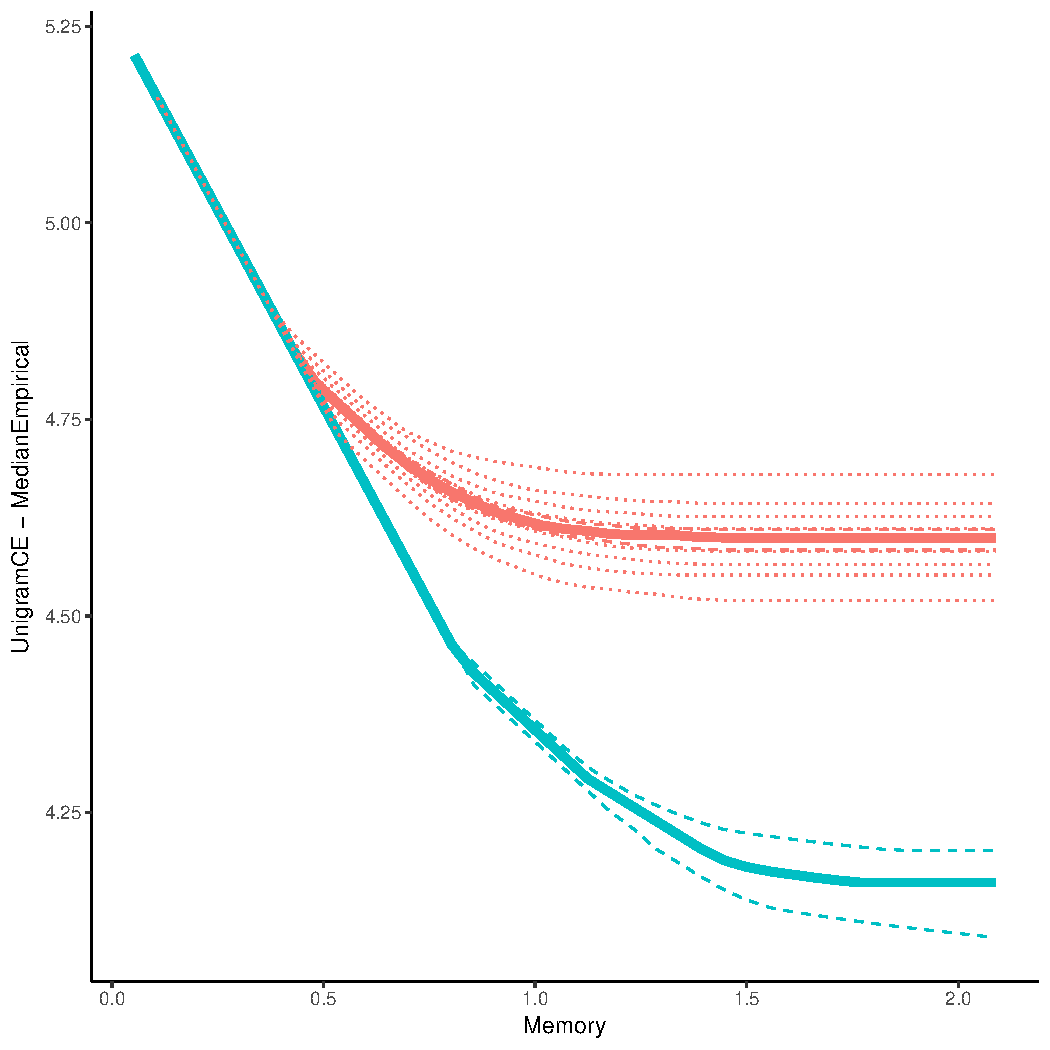
\includegraphics[width=0.25\textwidth]{neural/figures/Amharic-Adap-listener-surprisal-memory-MEDIANS_QUANTILES_onlyWordForms_boundedVocab_REAL.pdf} & 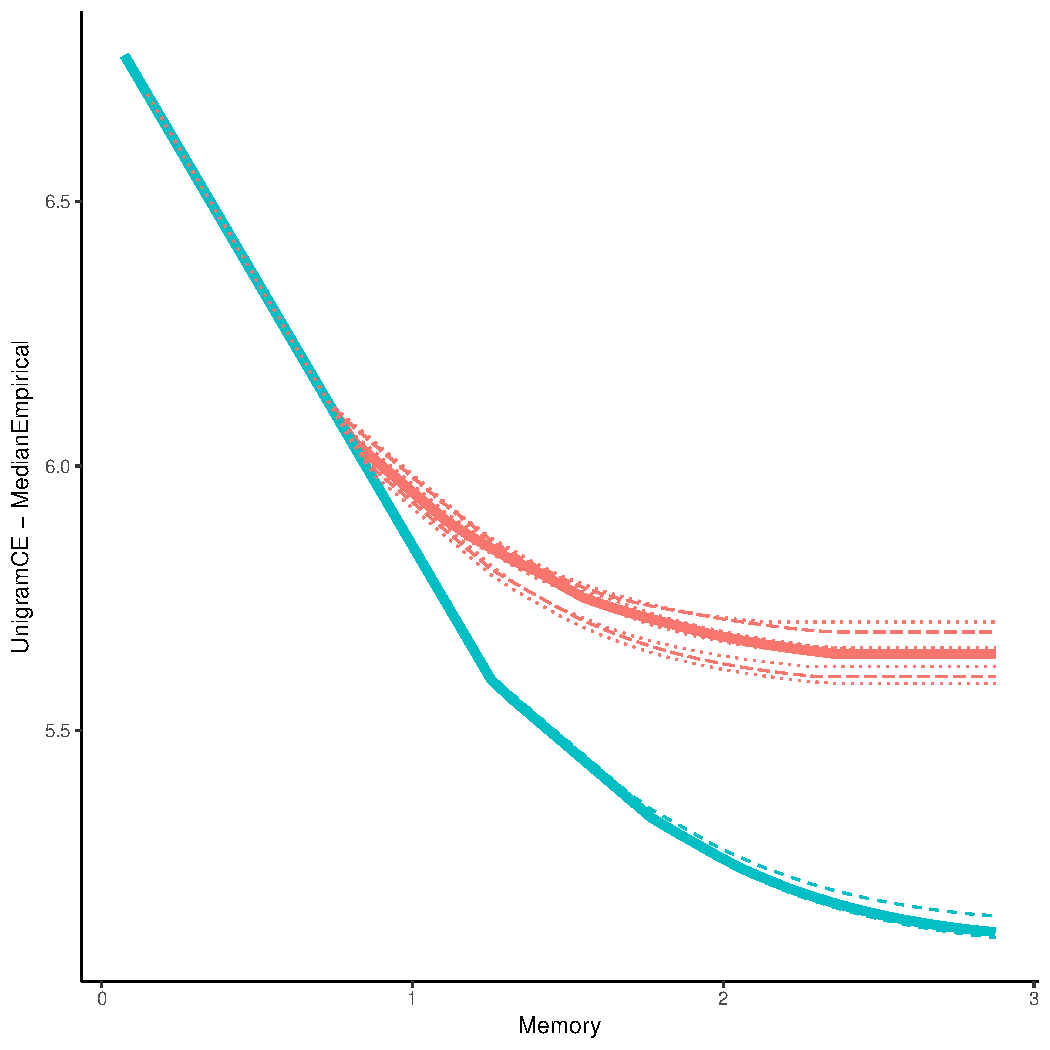
\includegraphics[width=0.25\textwidth]{neural/figures/Arabic-listener-surprisal-memory-MEDIANS_QUANTILES_onlyWordForms_boundedVocab_REAL.pdf} & 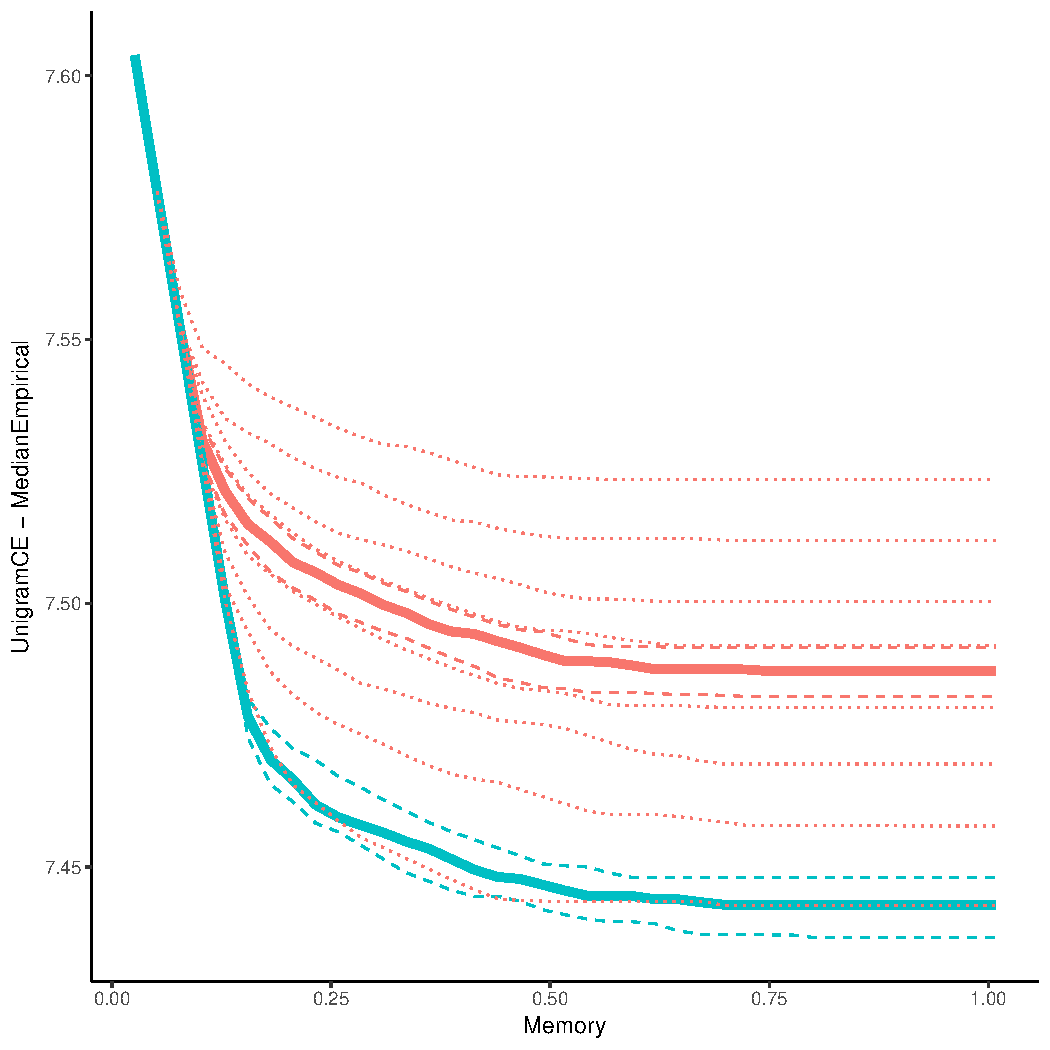
\includegraphics[width=0.25\textwidth]{neural/figures/Armenian-Adap-listener-surprisal-memory-MEDIANS_QUANTILES_onlyWordForms_boundedVocab_REAL.pdf}
 \\ 
Bambara & Basque & Breton & Bulgarian
 \\ 
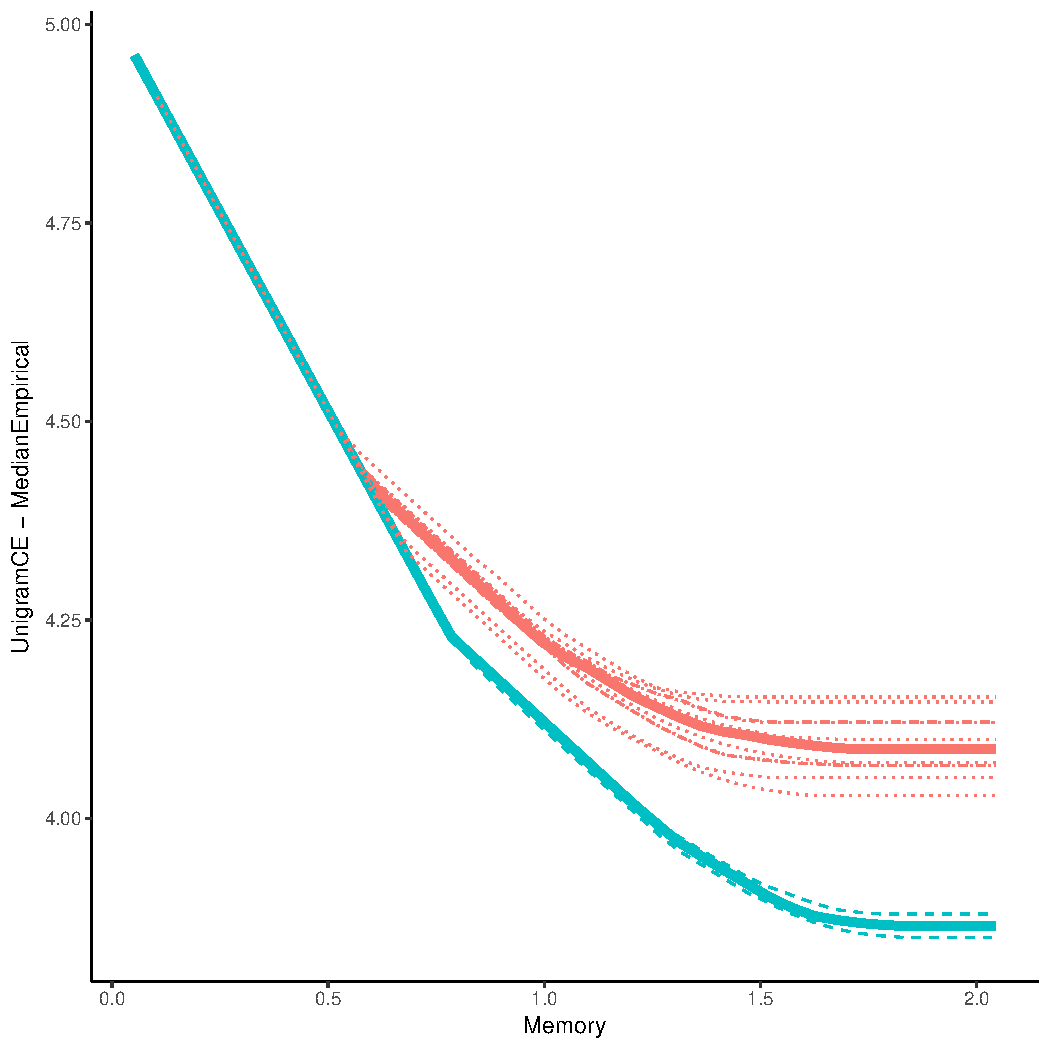
\includegraphics[width=0.25\textwidth]{neural/figures/Bambara-Adap-listener-surprisal-memory-MEDIANS_QUANTILES_onlyWordForms_boundedVocab_REAL.pdf} & 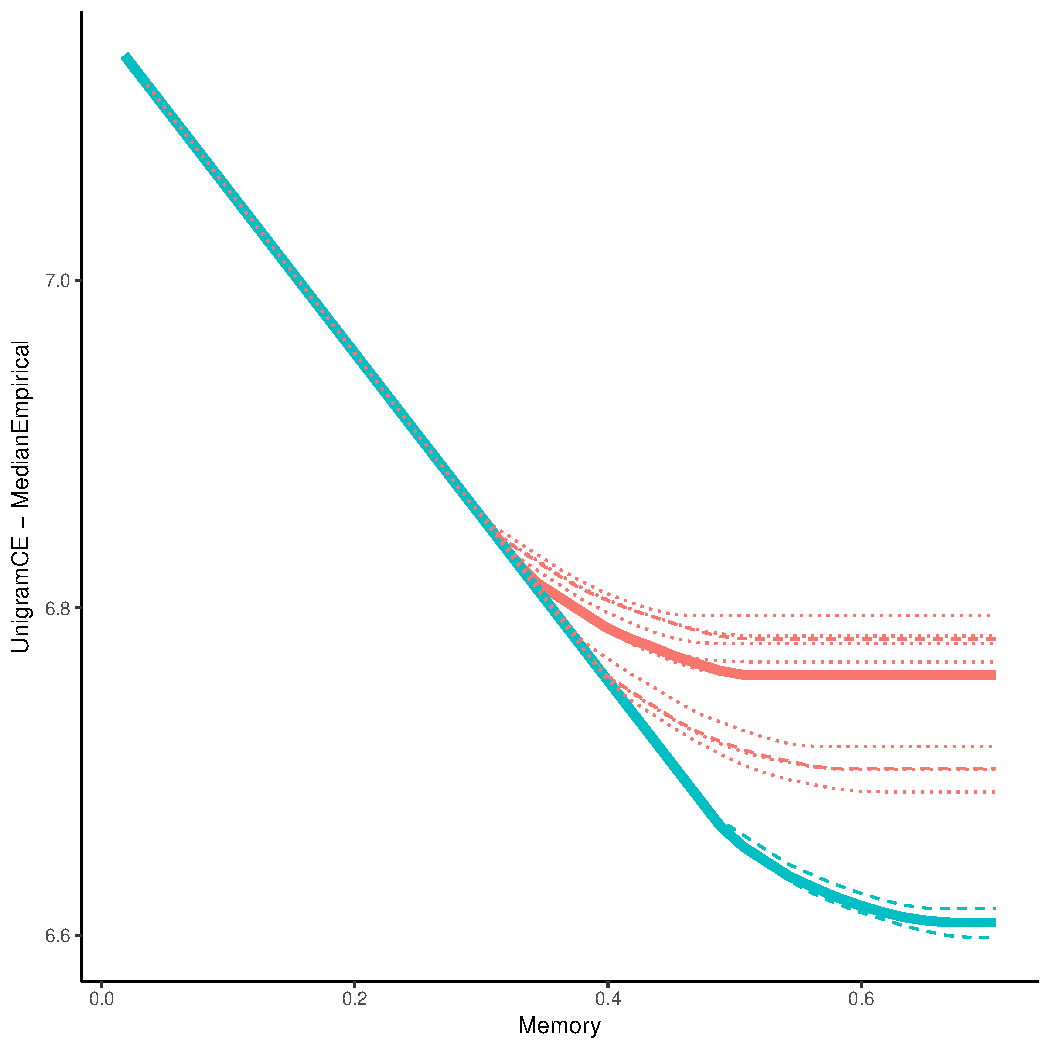
\includegraphics[width=0.25\textwidth]{neural/figures/Basque-listener-surprisal-memory-MEDIANS_QUANTILES_onlyWordForms_boundedVocab_REAL.pdf} & 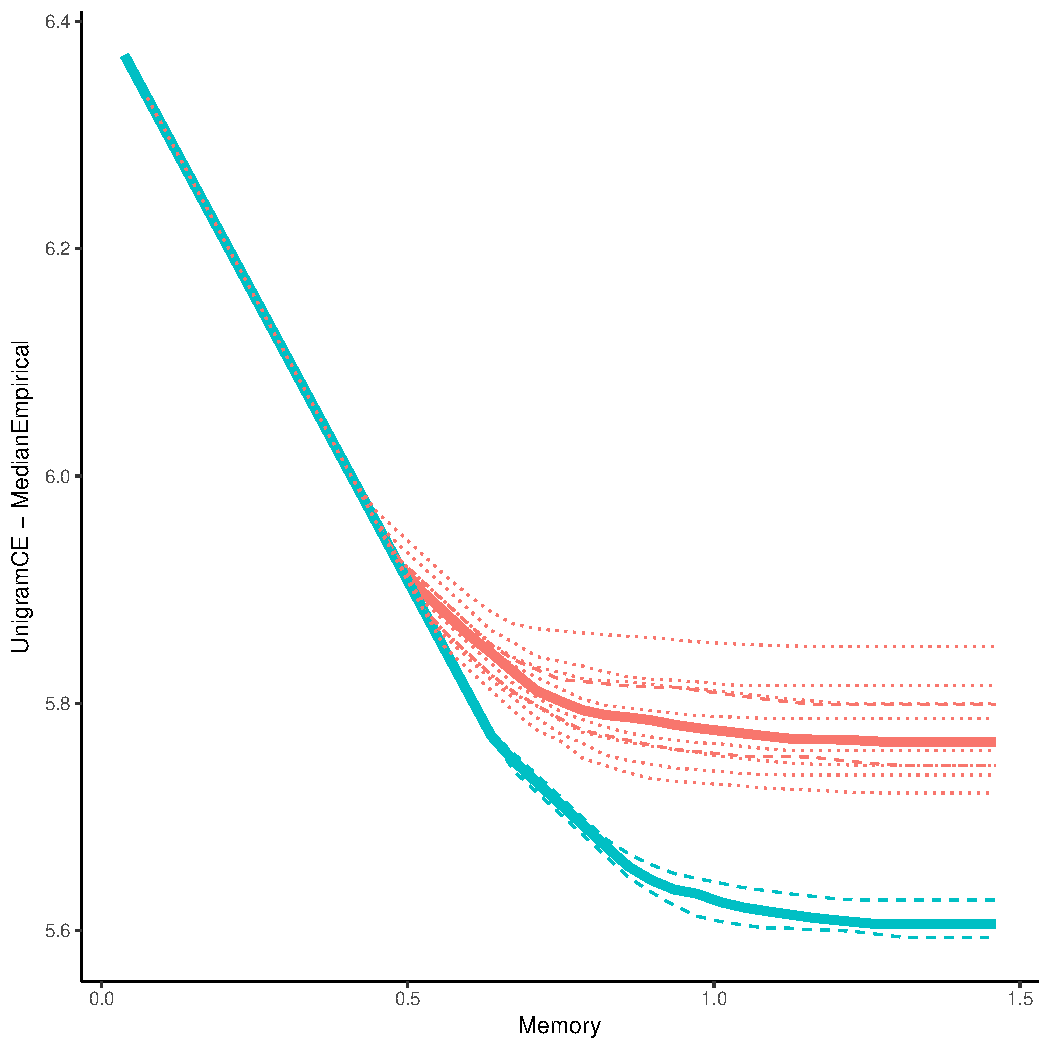
\includegraphics[width=0.25\textwidth]{neural/figures/Breton-Adap-listener-surprisal-memory-MEDIANS_QUANTILES_onlyWordForms_boundedVocab_REAL.pdf} & 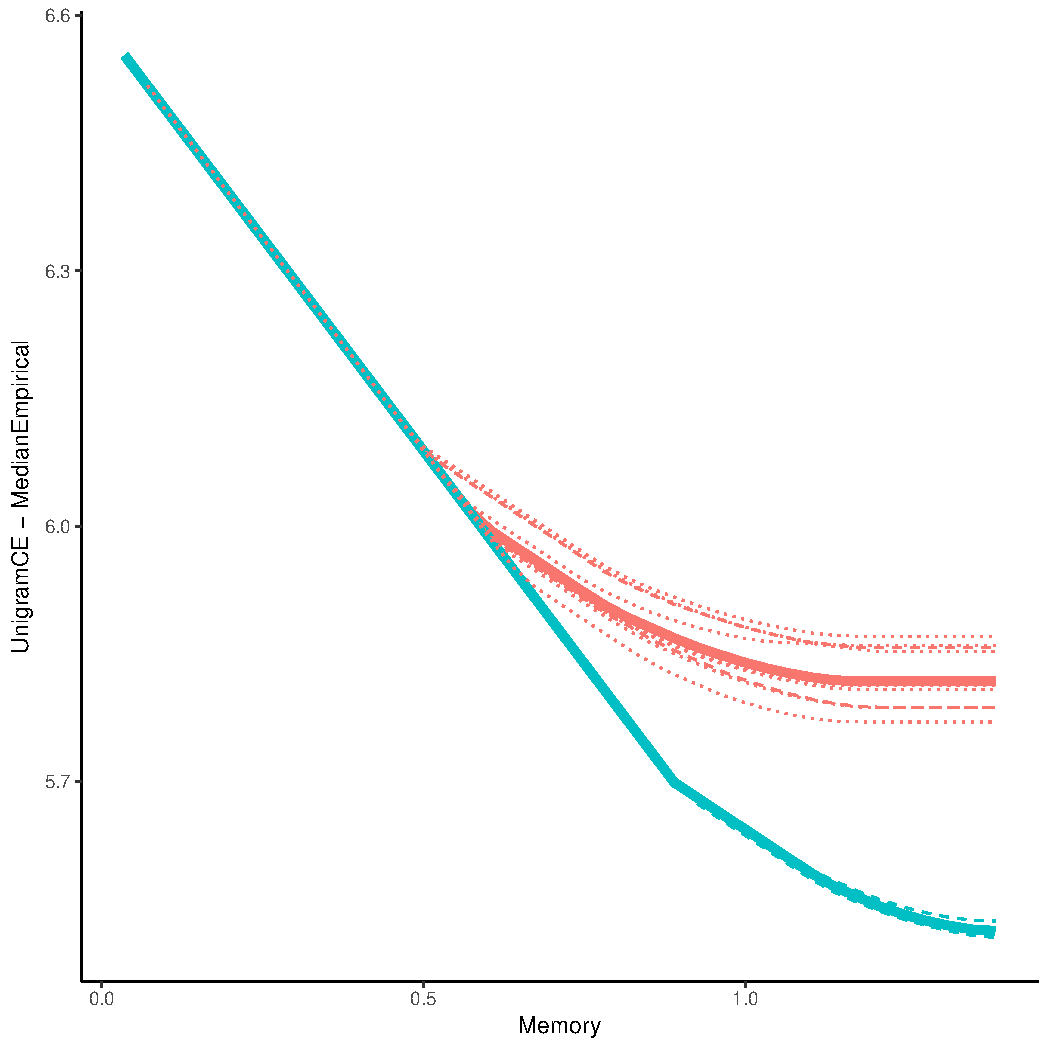
\includegraphics[width=0.25\textwidth]{neural/figures/Bulgarian-listener-surprisal-memory-MEDIANS_QUANTILES_onlyWordForms_boundedVocab_REAL.pdf}
 \\ 
Buryat & Cantonese & Catalan & Chinese
 \\ 
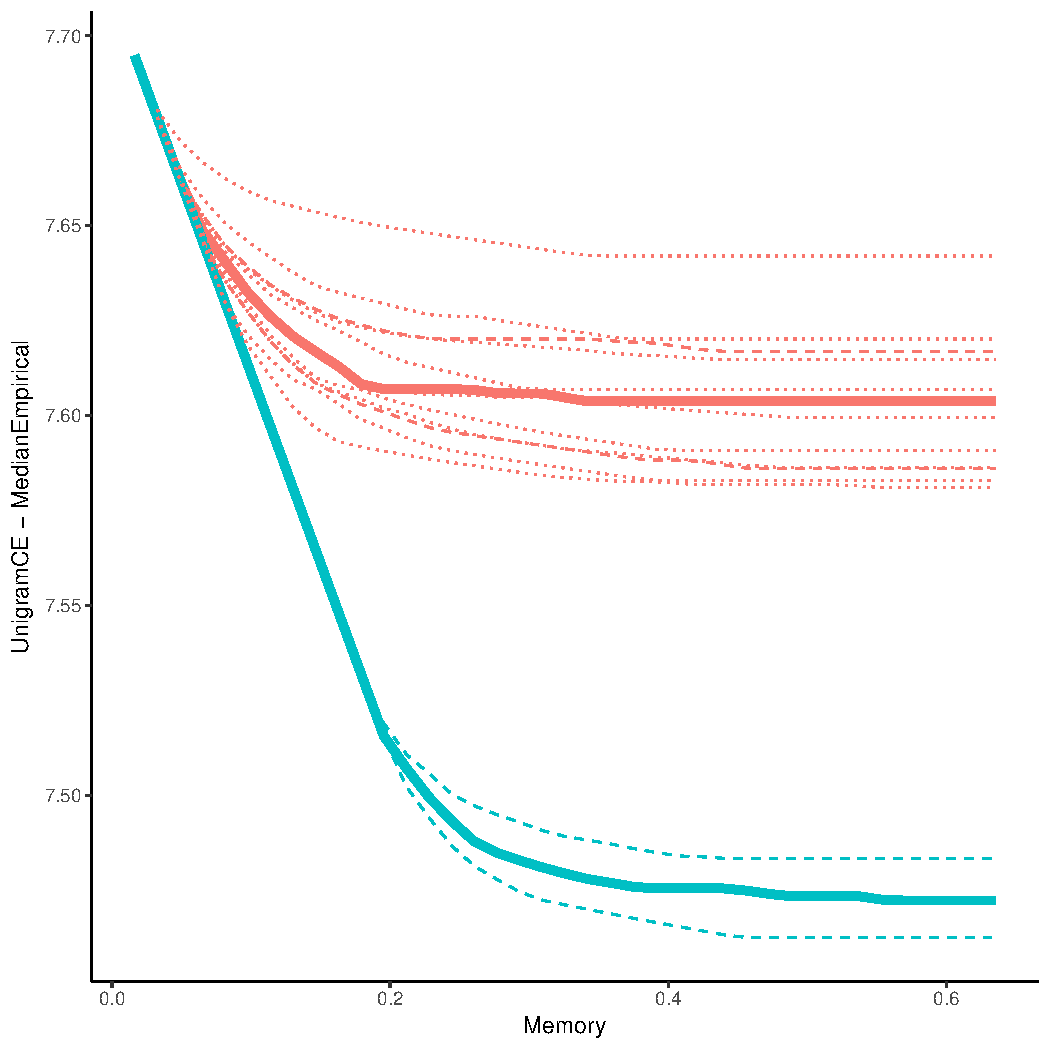
\includegraphics[width=0.25\textwidth]{neural/figures/Buryat-Adap-listener-surprisal-memory-MEDIANS_QUANTILES_onlyWordForms_boundedVocab_REAL.pdf} & 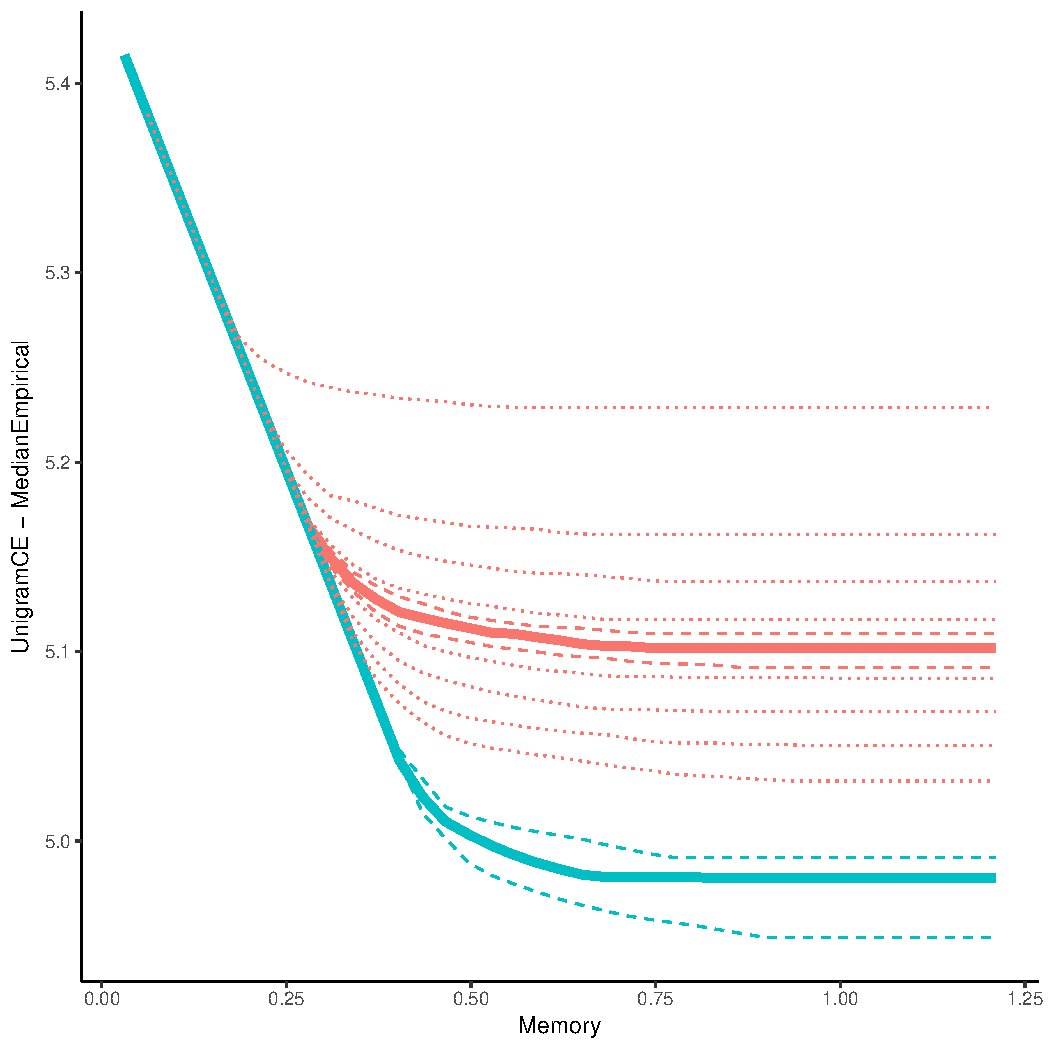
\includegraphics[width=0.25\textwidth]{neural/figures/Cantonese-Adap-listener-surprisal-memory-MEDIANS_QUANTILES_onlyWordForms_boundedVocab_REAL.pdf} & 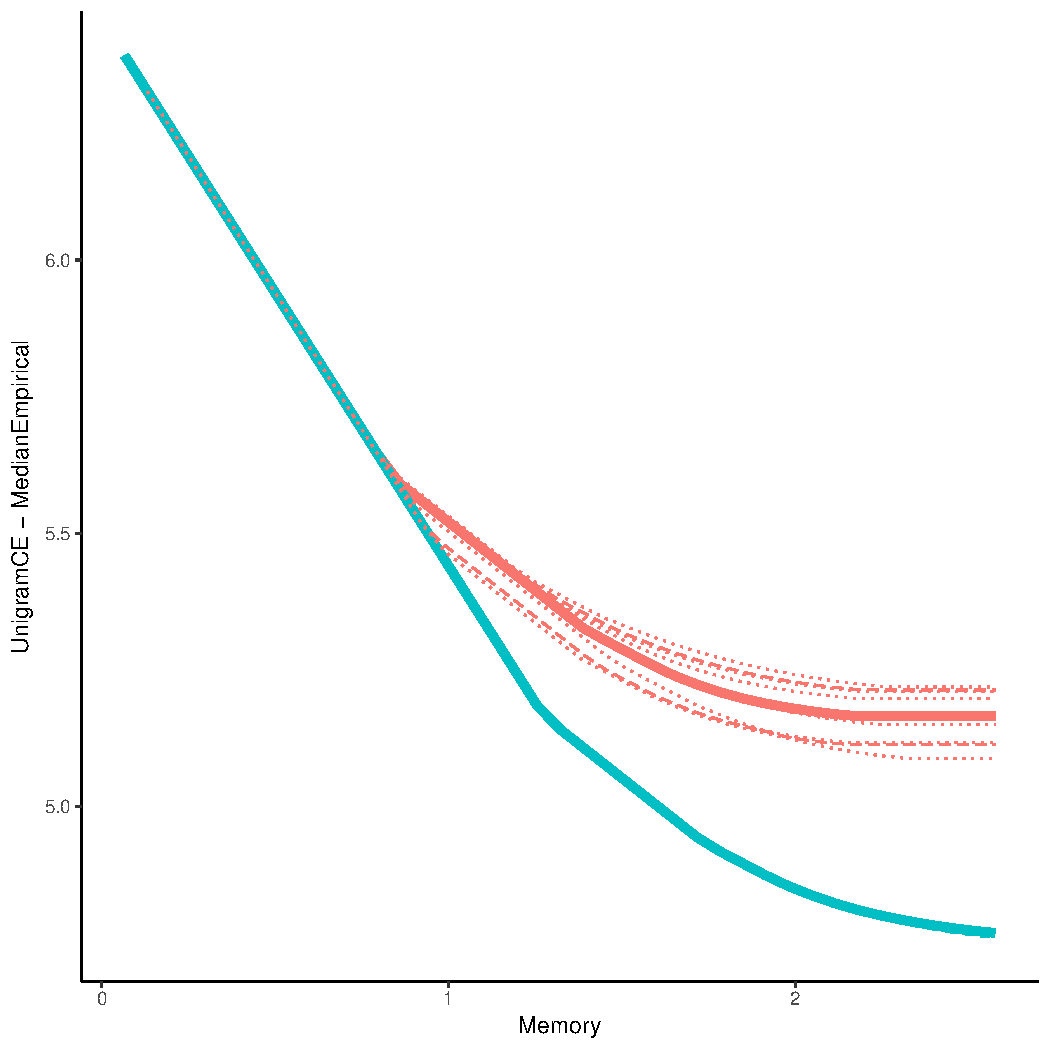
\includegraphics[width=0.25\textwidth]{neural/figures/Catalan-listener-surprisal-memory-MEDIANS_QUANTILES_onlyWordForms_boundedVocab_REAL.pdf} & 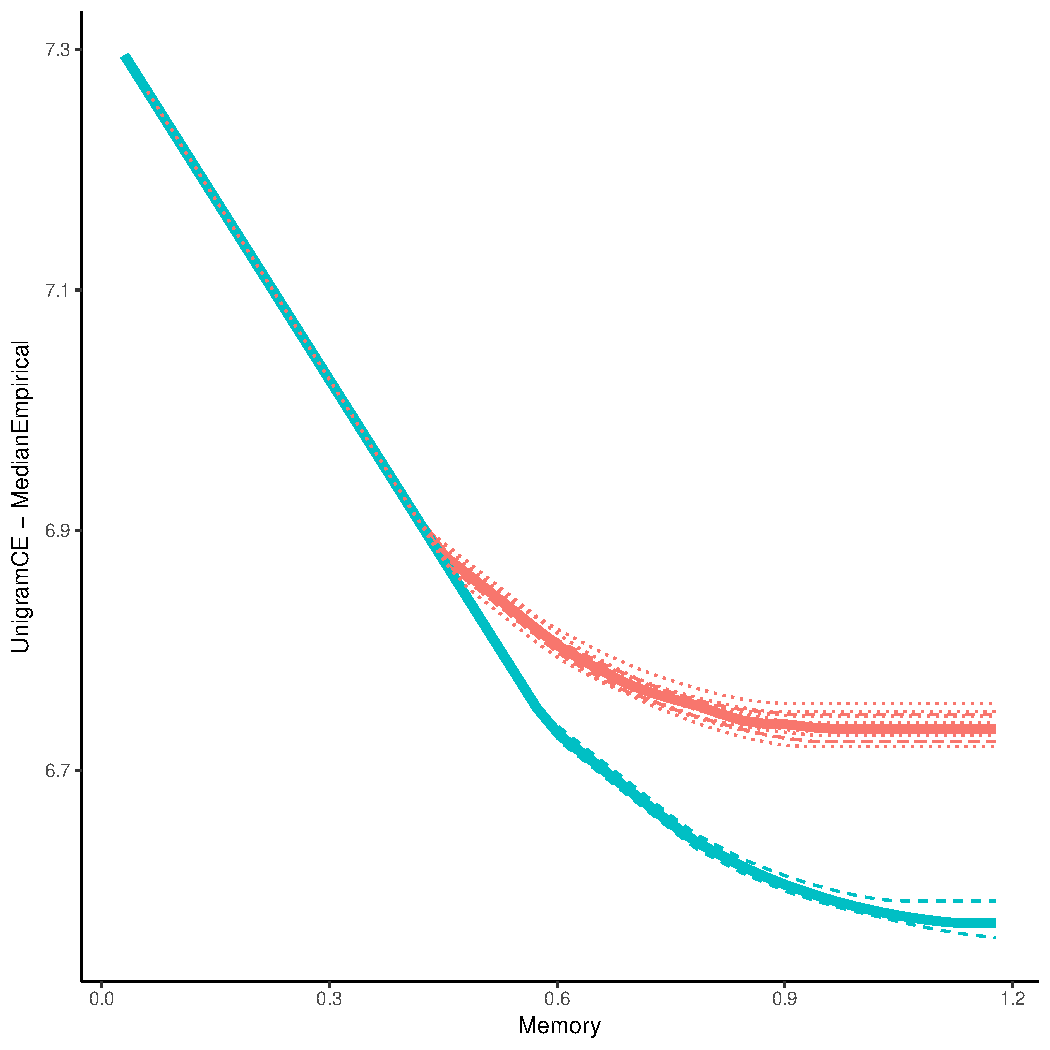
\includegraphics[width=0.25\textwidth]{neural/figures/Chinese-listener-surprisal-memory-MEDIANS_QUANTILES_onlyWordForms_boundedVocab_REAL.pdf}
 \\ 
Croatian & Czech & Danish & Dutch
 \\ 
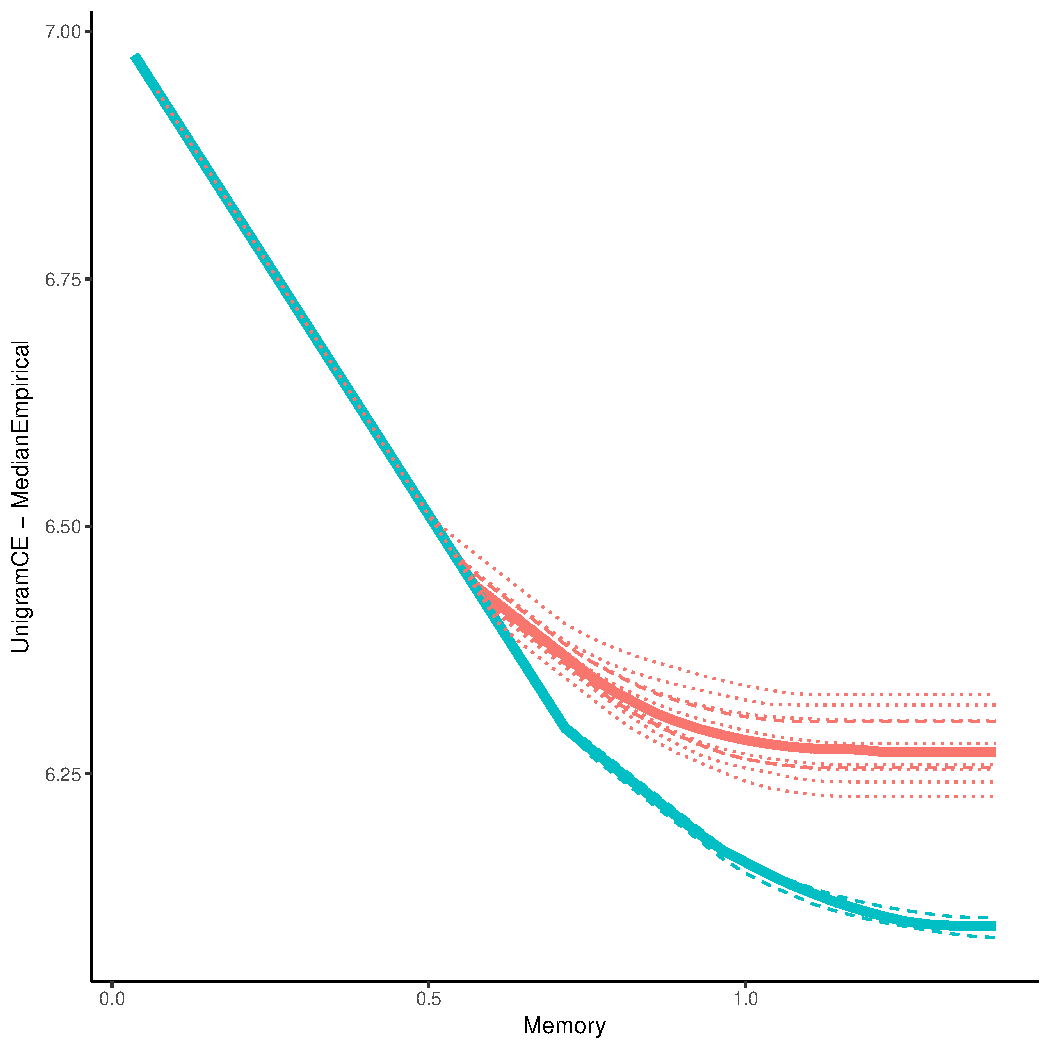
\includegraphics[width=0.25\textwidth]{neural/figures/Croatian-listener-surprisal-memory-MEDIANS_QUANTILES_onlyWordForms_boundedVocab_REAL.pdf} & 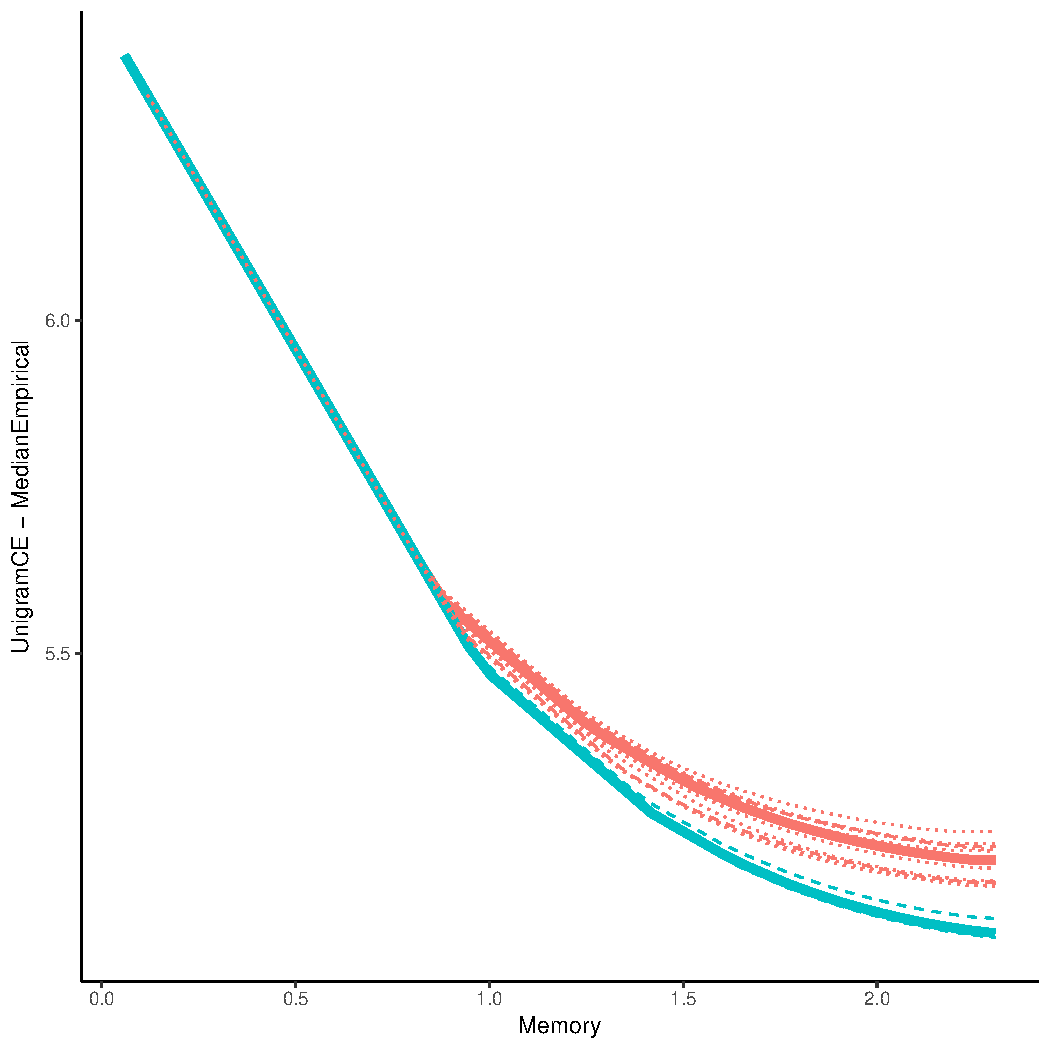
\includegraphics[width=0.25\textwidth]{neural/figures/Czech-listener-surprisal-memory-MEDIANS_QUANTILES_onlyWordForms_boundedVocab_REAL.pdf} & 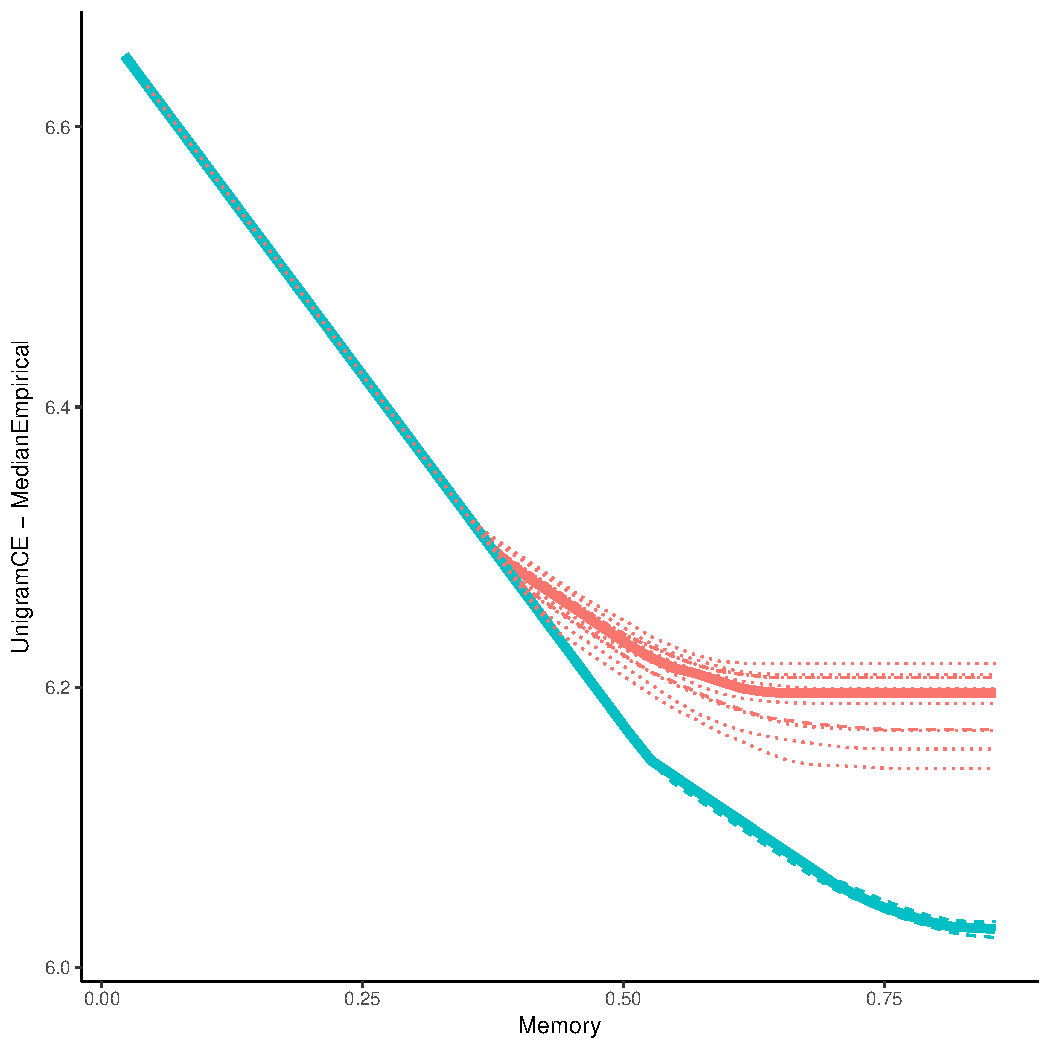
\includegraphics[width=0.25\textwidth]{neural/figures/Danish-listener-surprisal-memory-MEDIANS_QUANTILES_onlyWordForms_boundedVocab_REAL.pdf} & 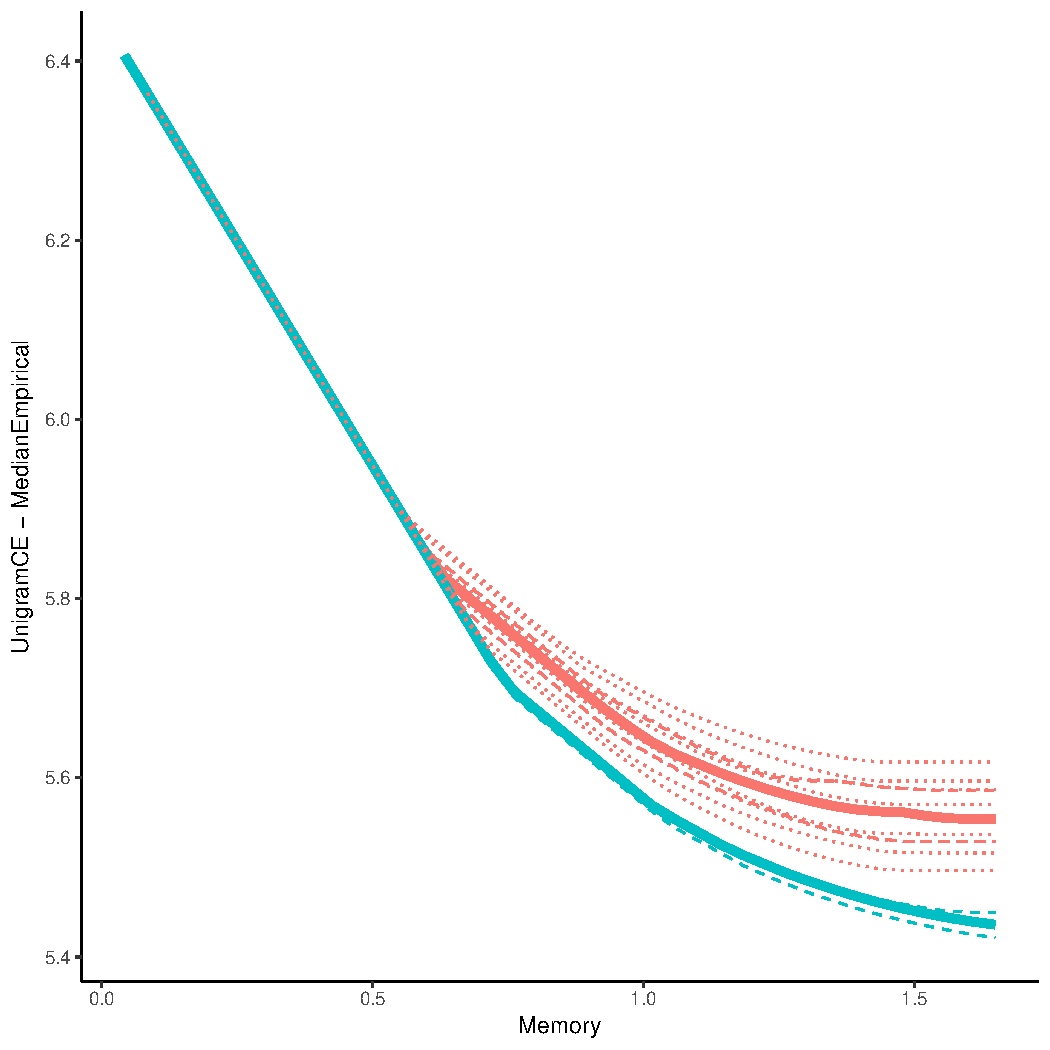
\includegraphics[width=0.25\textwidth]{neural/figures/Dutch-listener-surprisal-memory-MEDIANS_QUANTILES_onlyWordForms_boundedVocab_REAL.pdf}
 \\ 

\end{longtable}
	\caption{Medians: For each memory budget, we provide the median surprisal for real and random languages. Solid lines indicate sample medians, dashed lines indicate 95 $\%$ confidence intervals for the population median. Green: Random baselines; blue: real language; red: maximum-likelihood grammars fit to real orderings.}\label{tab:medians}
\end{table}

\begin{table}
\begin{longtable}{ccccccccccccccclll}
English & Erzya & Estonian & Faroese
 \\ 
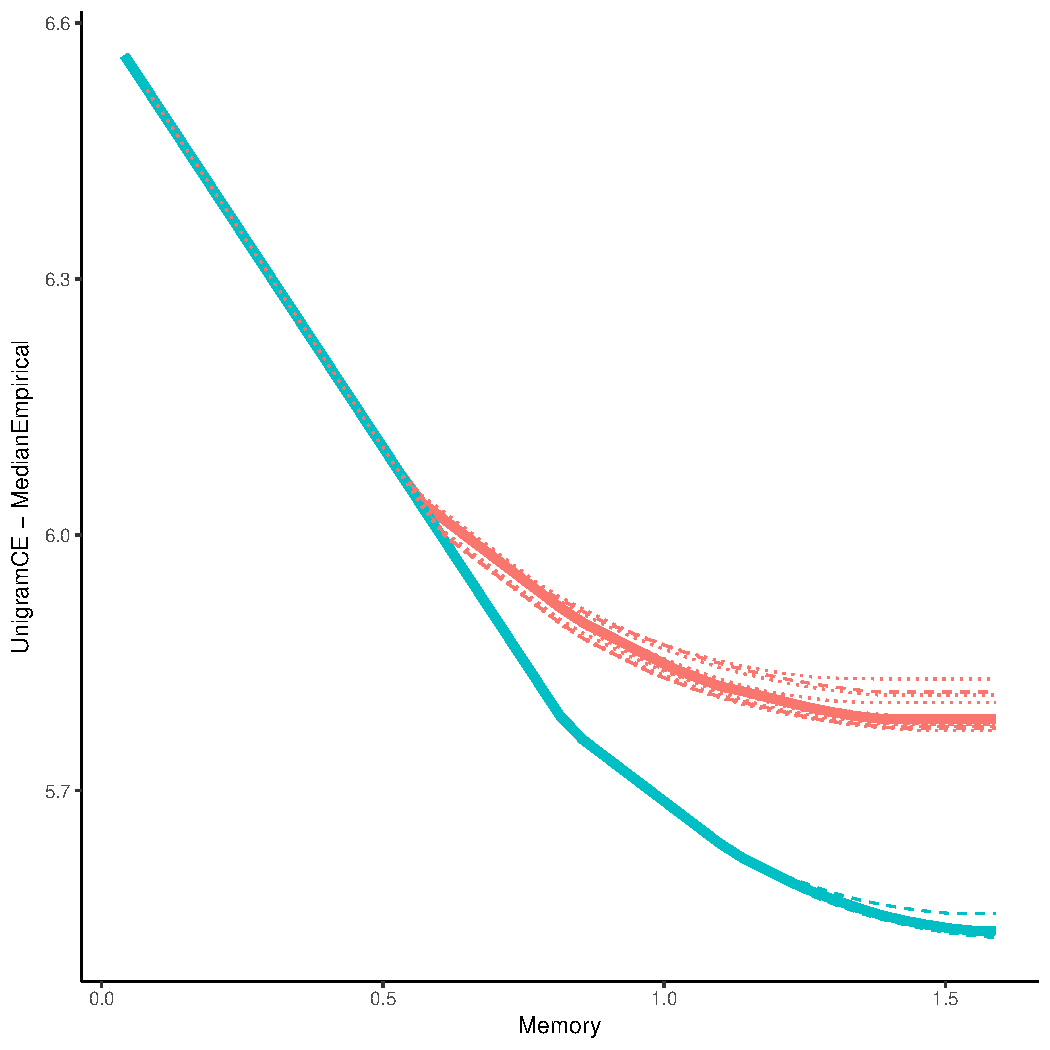
\includegraphics[width=0.25\textwidth]{neural/figures/English-listener-surprisal-memory-MEDIANS_QUANTILES_onlyWordForms_boundedVocab_REAL.pdf} & 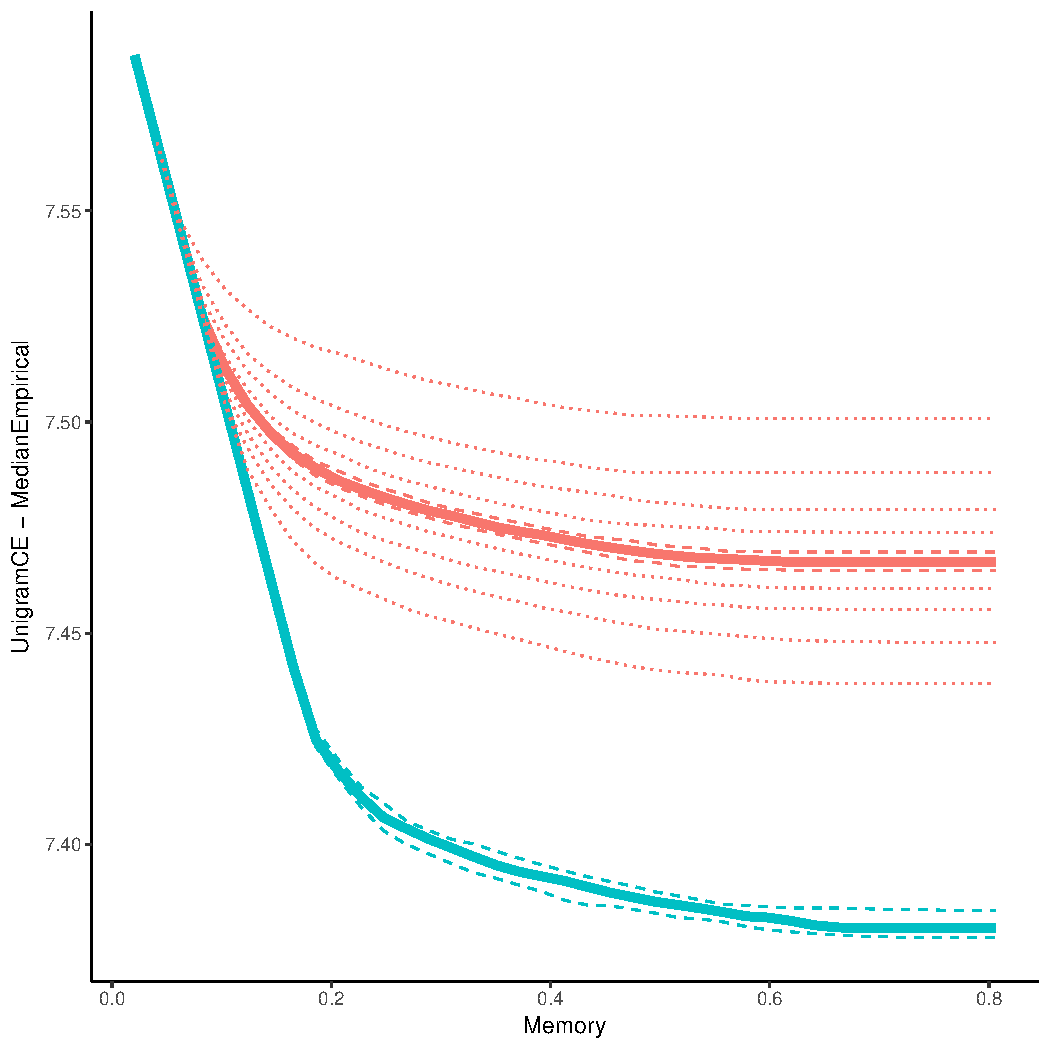
\includegraphics[width=0.25\textwidth]{neural/figures/Erzya-Adap-listener-surprisal-memory-MEDIANS_QUANTILES_onlyWordForms_boundedVocab_REAL.pdf} & 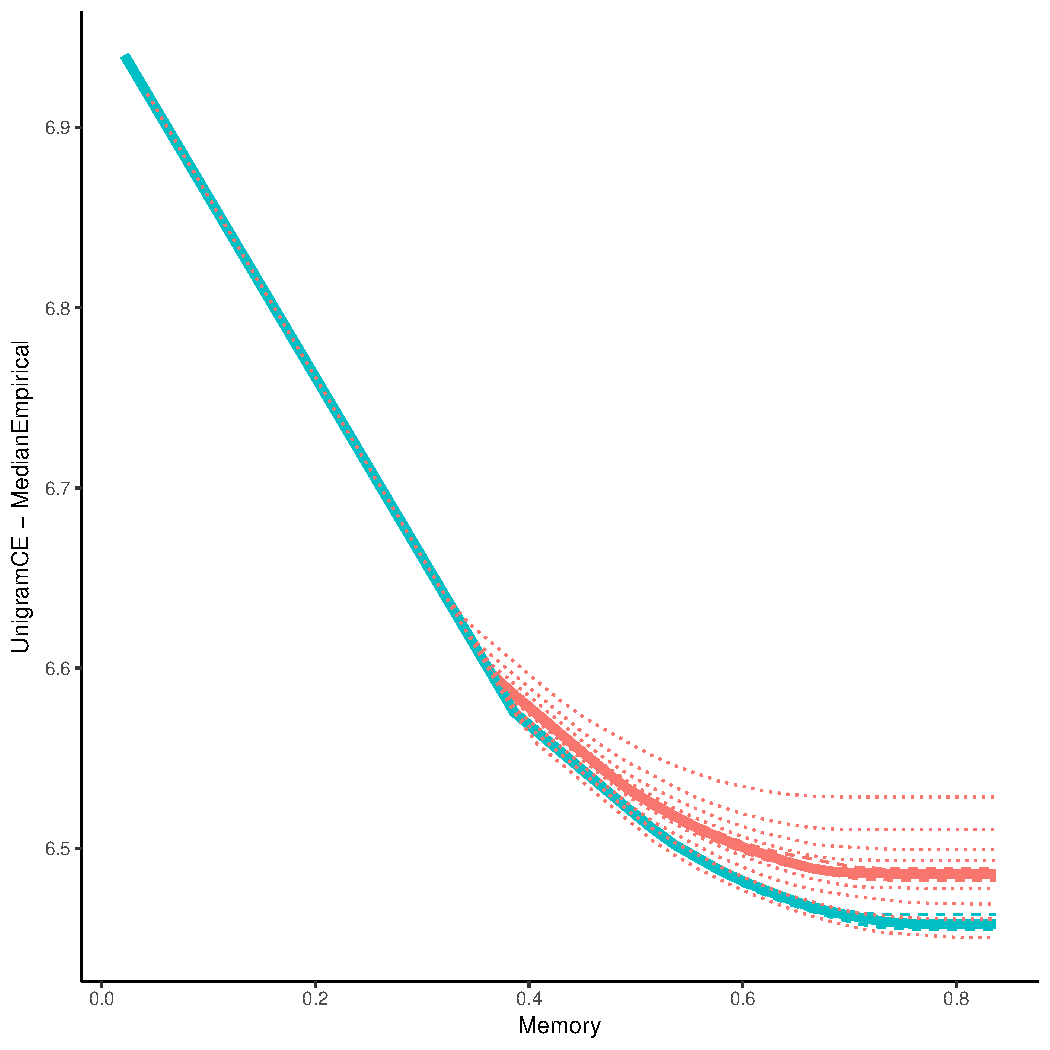
\includegraphics[width=0.25\textwidth]{neural/figures/Estonian-listener-surprisal-memory-MEDIANS_QUANTILES_onlyWordForms_boundedVocab_REAL.pdf} & 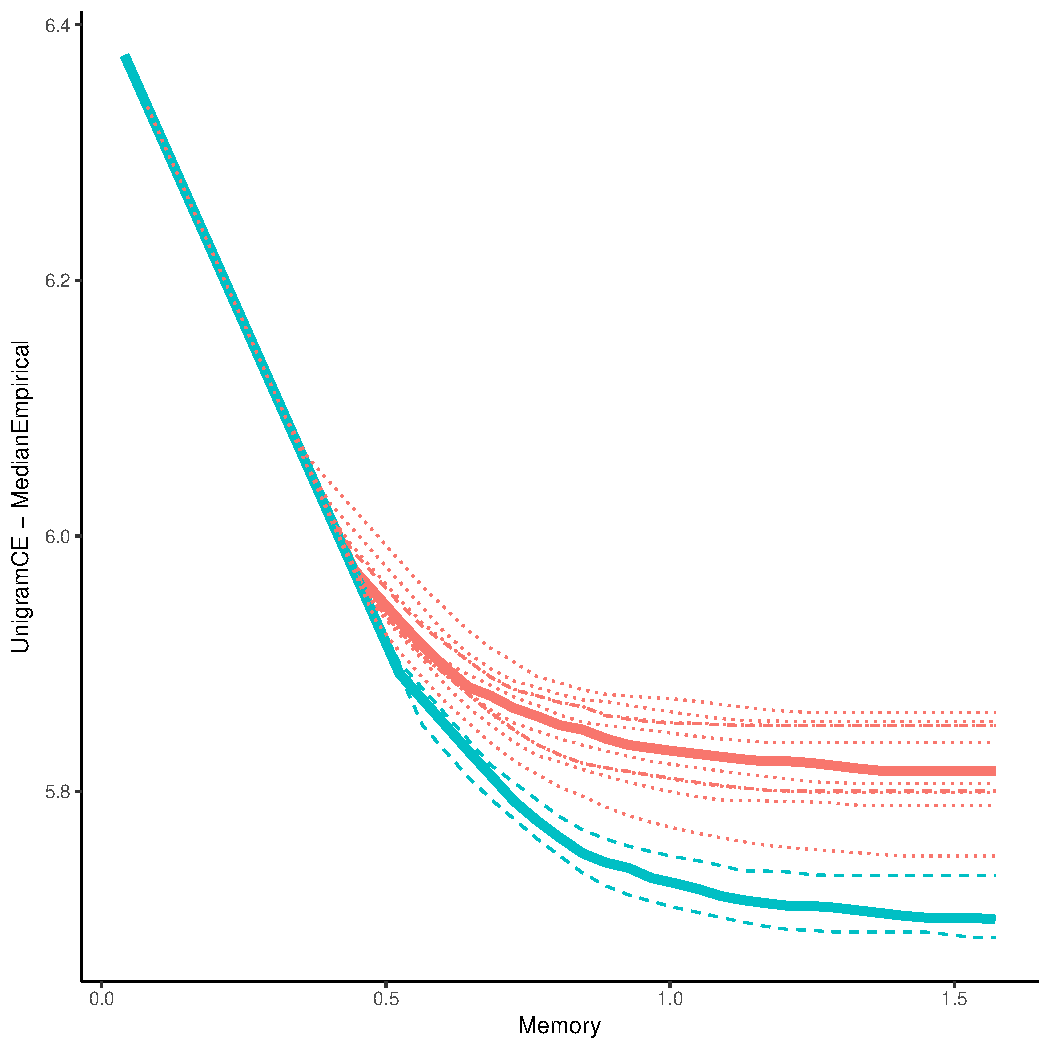
\includegraphics[width=0.25\textwidth]{neural/figures/Faroese-Adap-listener-surprisal-memory-MEDIANS_QUANTILES_onlyWordForms_boundedVocab_REAL.pdf}
 \\ 
Finnish & French & German & Greek
 \\ 
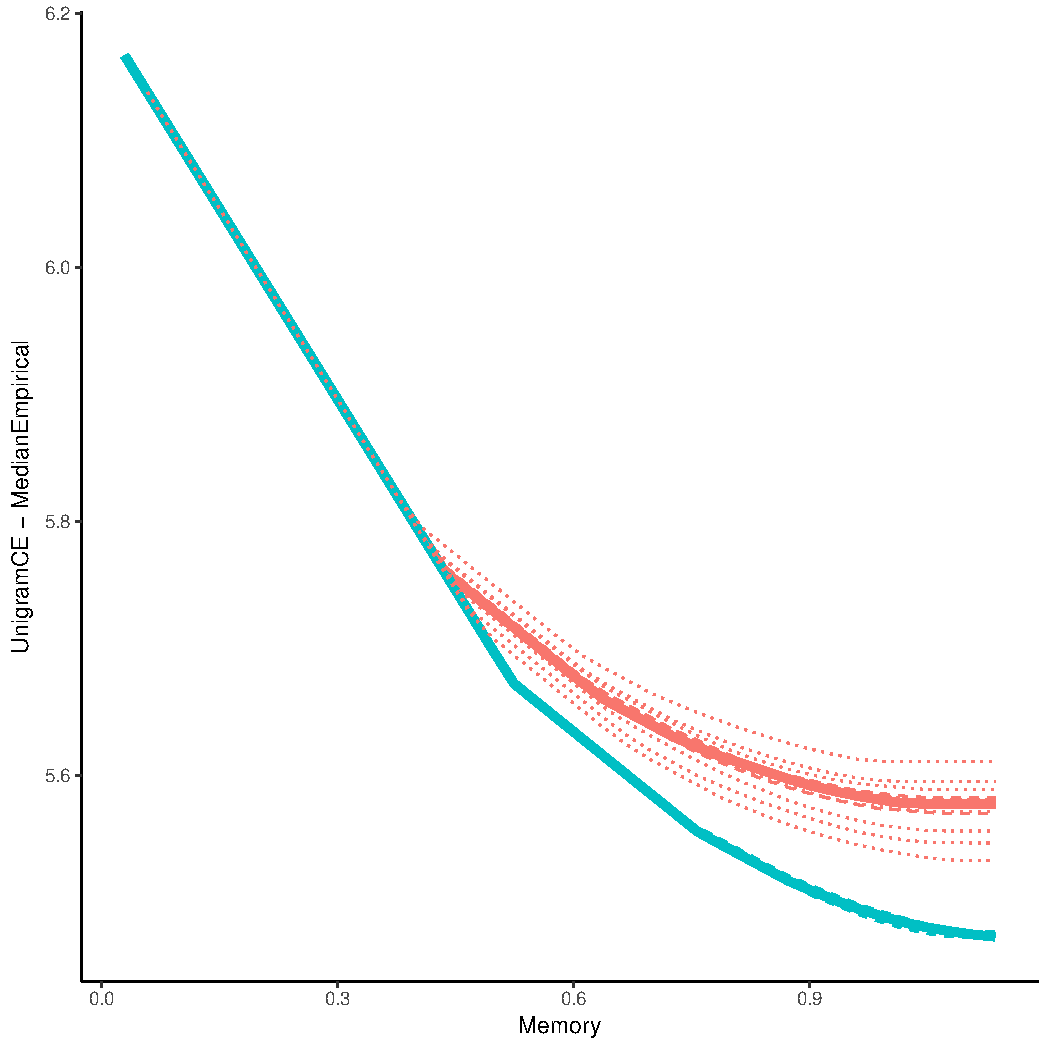
\includegraphics[width=0.25\textwidth]{neural/figures/Finnish-listener-surprisal-memory-MEDIANS_QUANTILES_onlyWordForms_boundedVocab_REAL.pdf} & 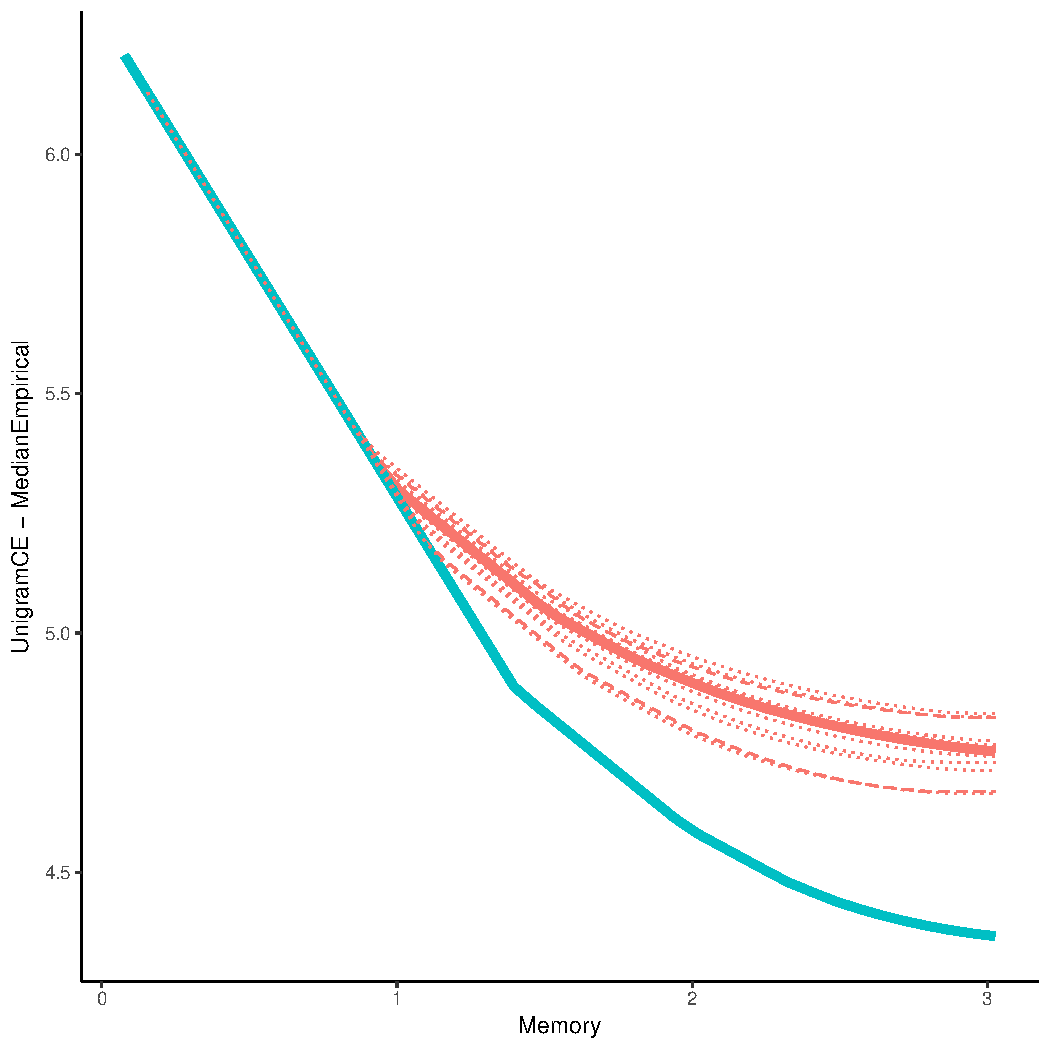
\includegraphics[width=0.25\textwidth]{neural/figures/French-listener-surprisal-memory-MEDIANS_QUANTILES_onlyWordForms_boundedVocab_REAL.pdf} & 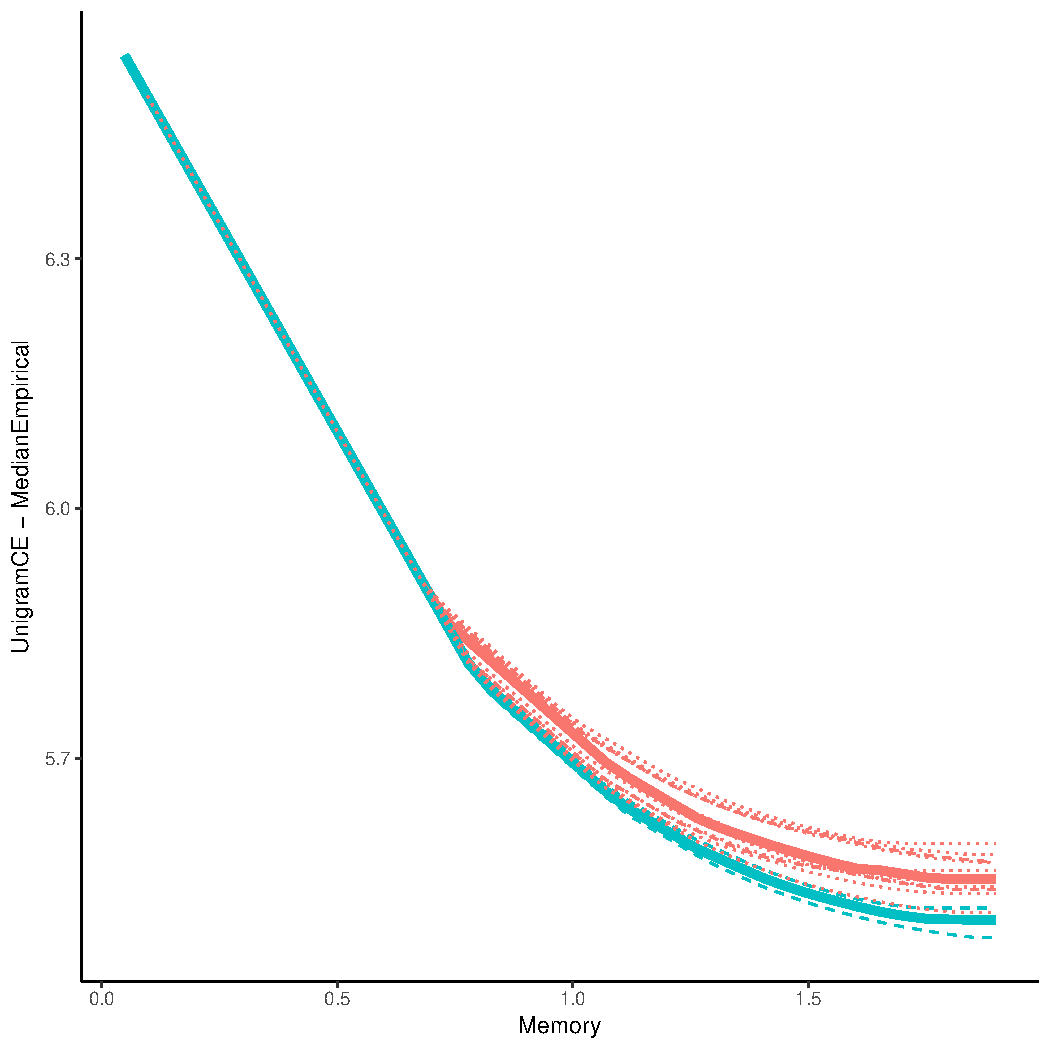
\includegraphics[width=0.25\textwidth]{neural/figures/German-listener-surprisal-memory-MEDIANS_QUANTILES_onlyWordForms_boundedVocab_REAL.pdf} & 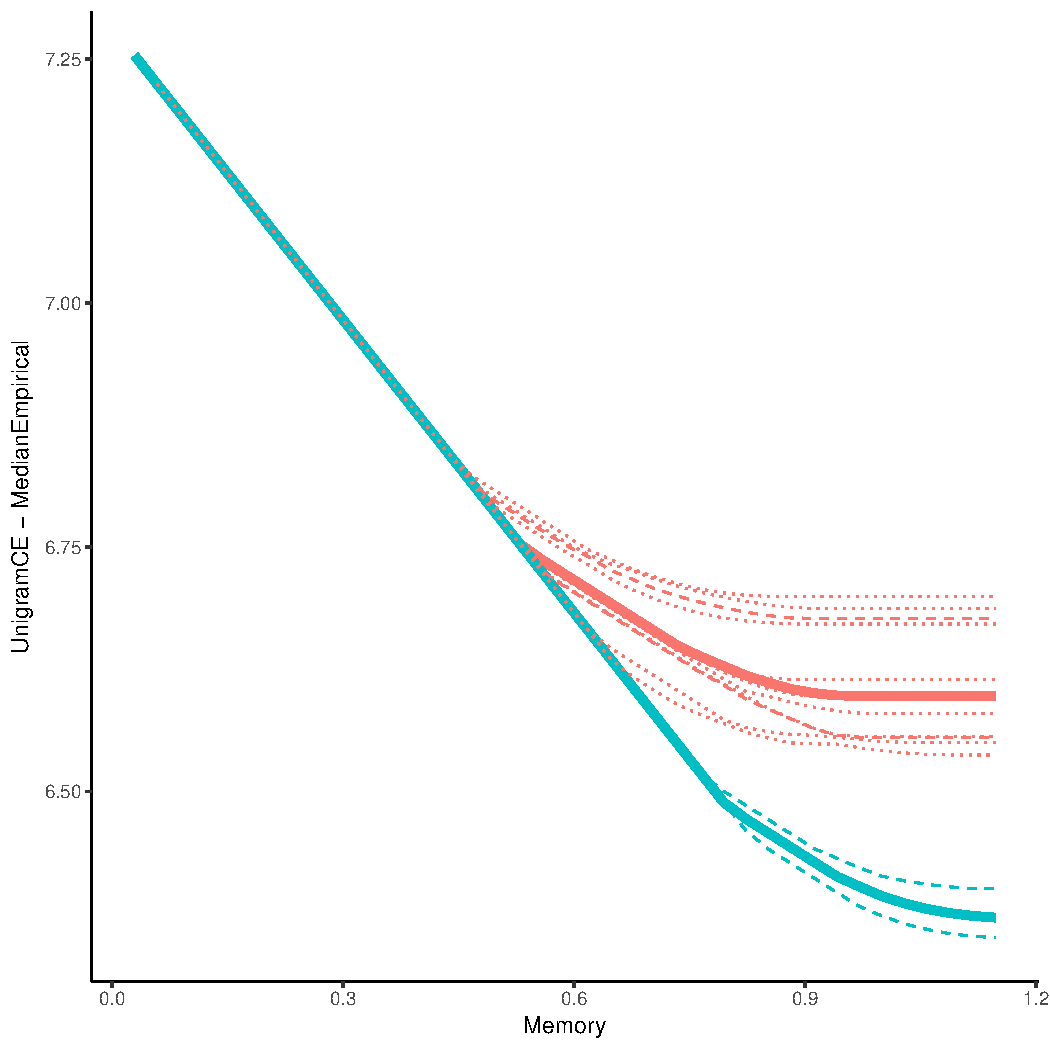
\includegraphics[width=0.25\textwidth]{neural/figures/Greek-listener-surprisal-memory-MEDIANS_QUANTILES_onlyWordForms_boundedVocab_REAL.pdf}
 \\ 
Hebrew & Hindi & Hungarian & Indonesian
 \\ 
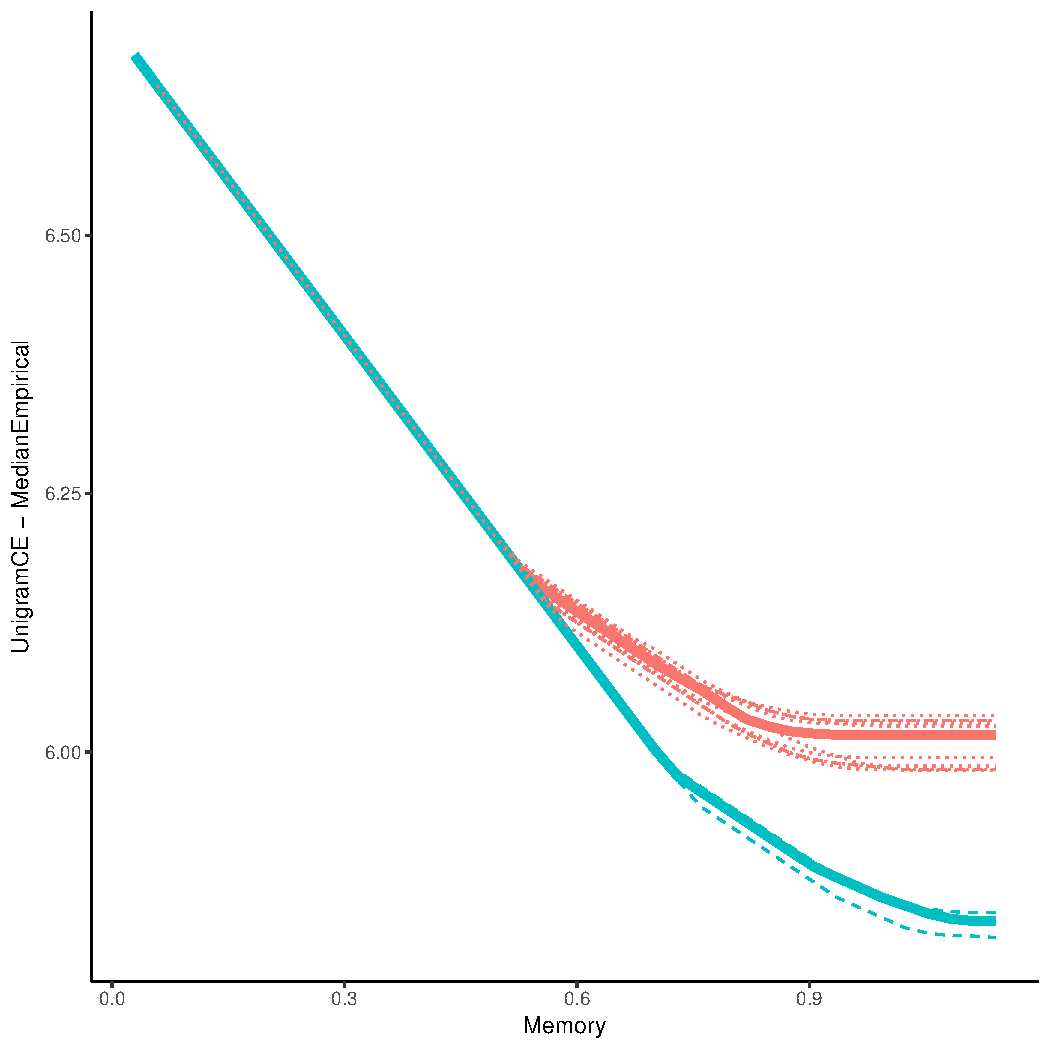
\includegraphics[width=0.25\textwidth]{neural/figures/Hebrew-listener-surprisal-memory-MEDIANS_QUANTILES_onlyWordForms_boundedVocab_REAL.pdf} & 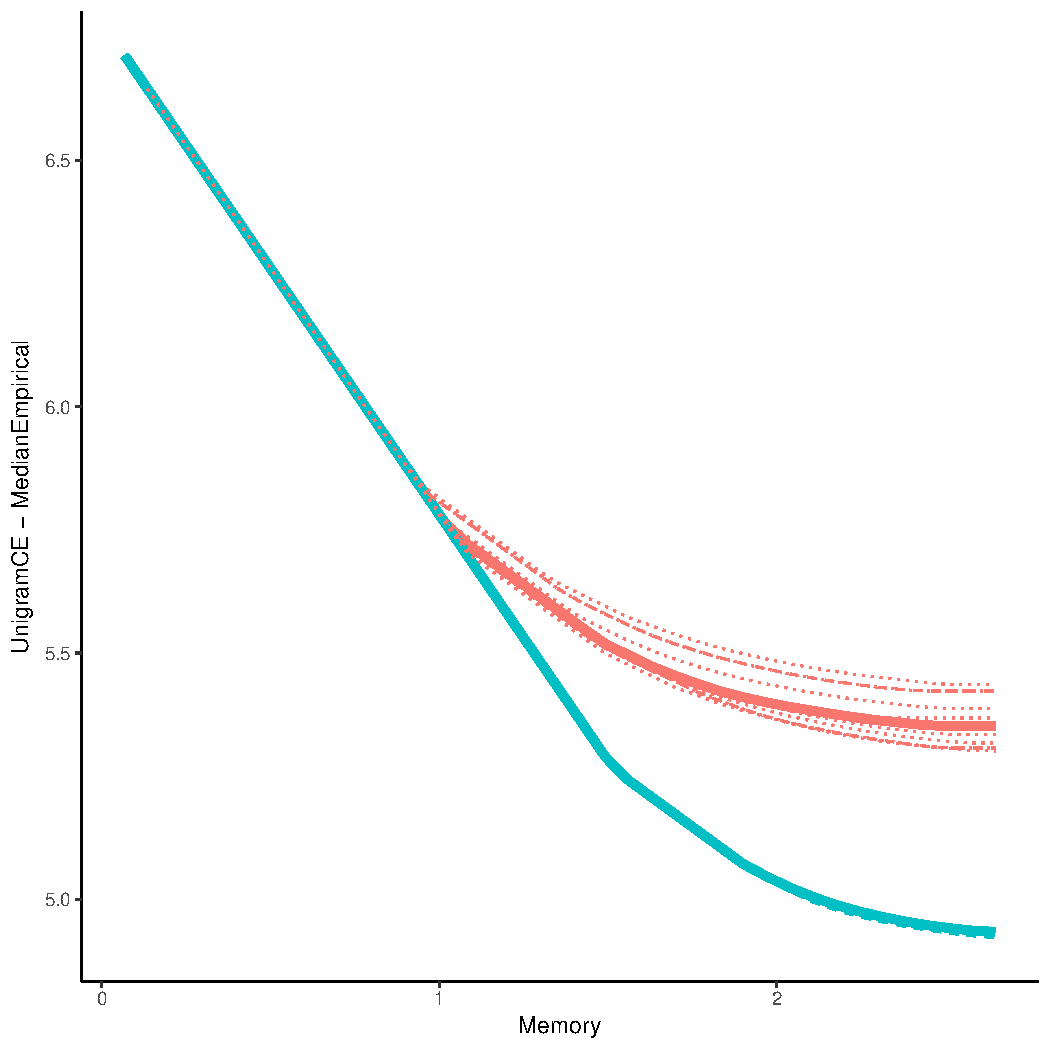
\includegraphics[width=0.25\textwidth]{neural/figures/Hindi-listener-surprisal-memory-MEDIANS_QUANTILES_onlyWordForms_boundedVocab_REAL.pdf} & 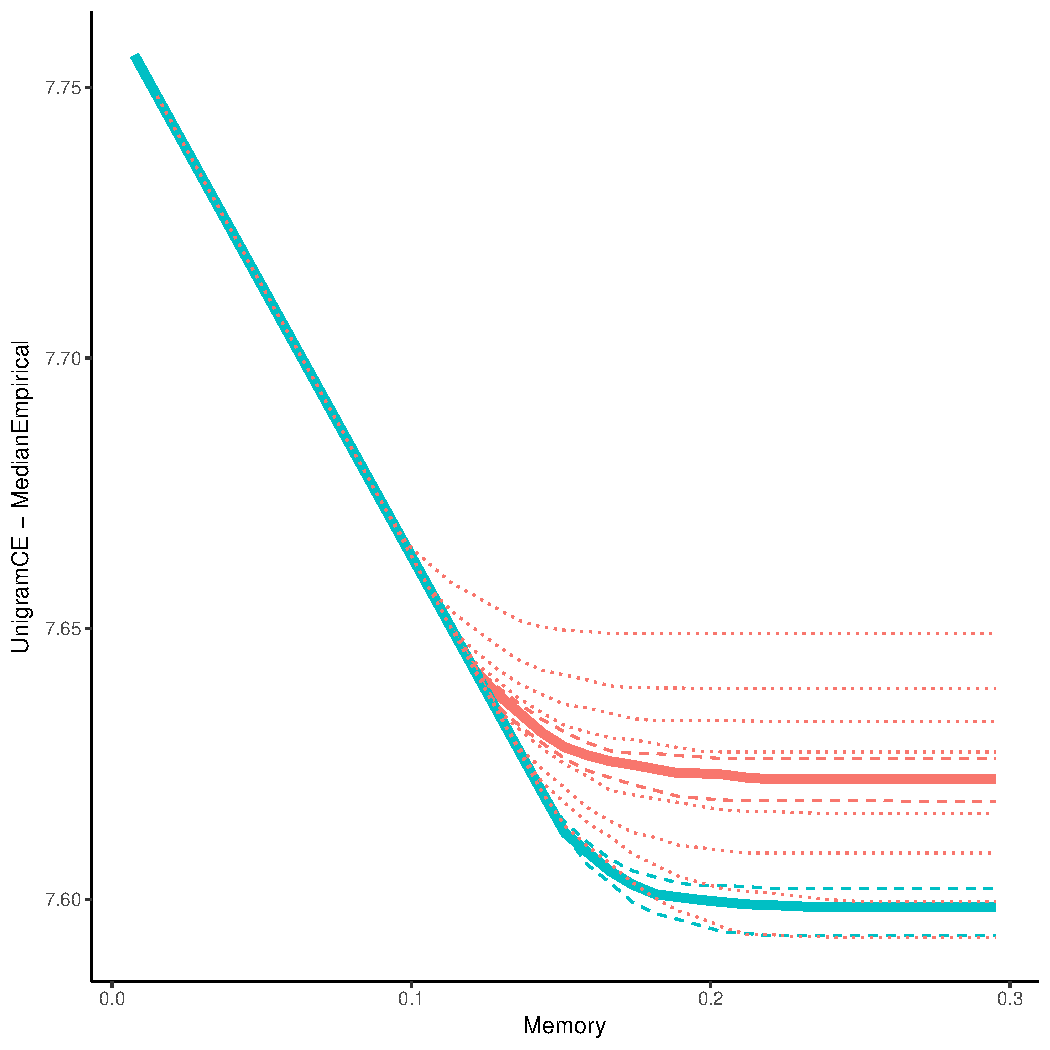
\includegraphics[width=0.25\textwidth]{neural/figures/Hungarian-listener-surprisal-memory-MEDIANS_QUANTILES_onlyWordForms_boundedVocab_REAL.pdf} & 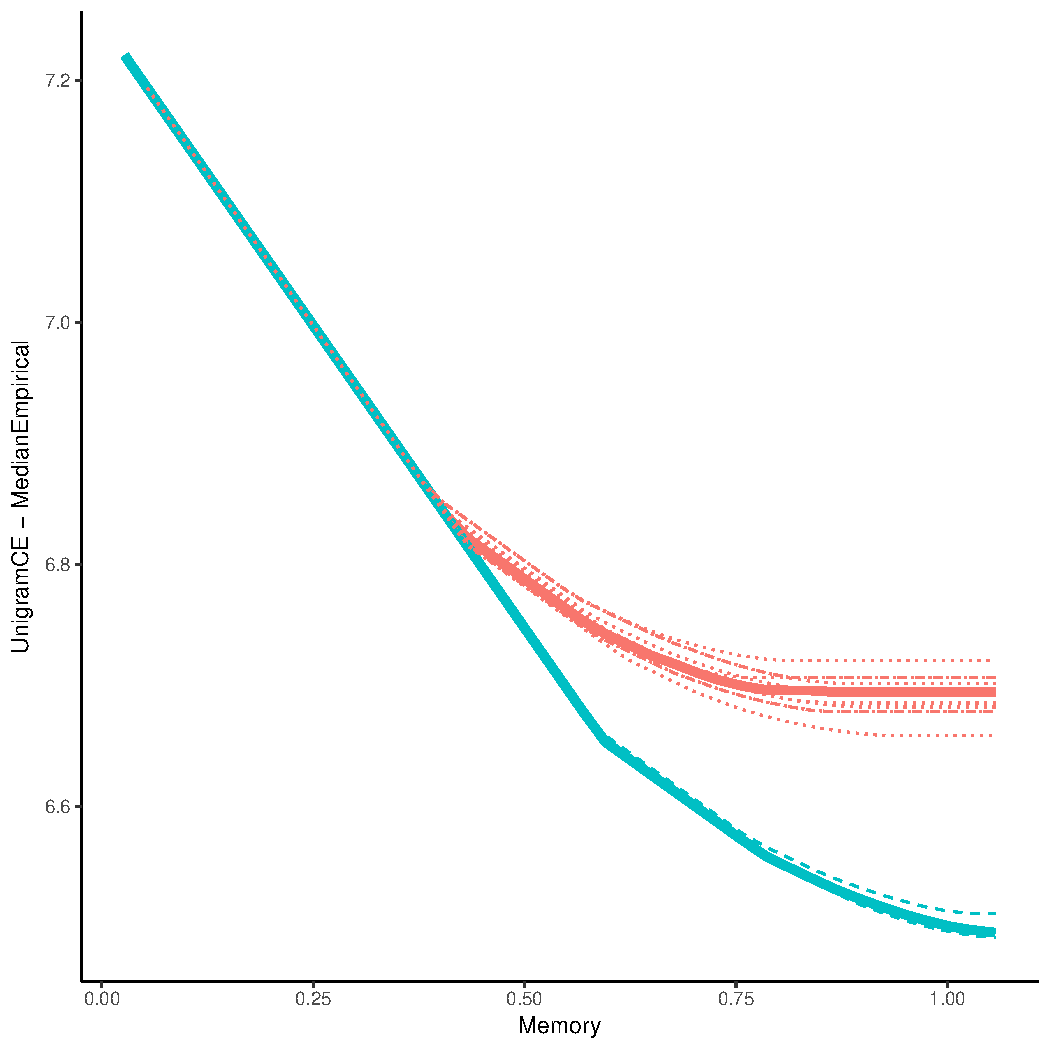
\includegraphics[width=0.25\textwidth]{neural/figures/Indonesian-listener-surprisal-memory-MEDIANS_QUANTILES_onlyWordForms_boundedVocab_REAL.pdf}
 \\ 
Italian & Japanese & Kazakh & Korean
 \\ 
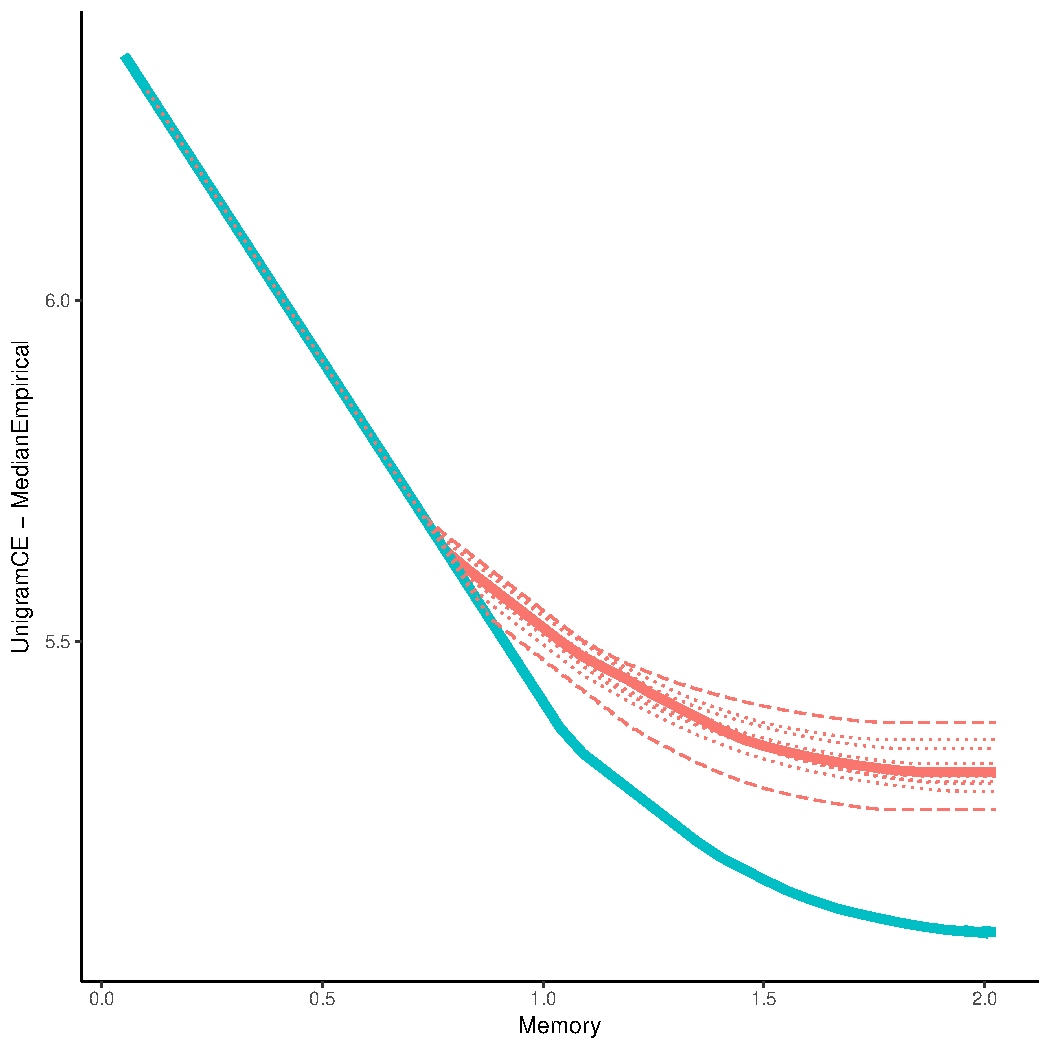
\includegraphics[width=0.25\textwidth]{neural/figures/Italian-listener-surprisal-memory-MEDIANS_QUANTILES_onlyWordForms_boundedVocab_REAL.pdf} & 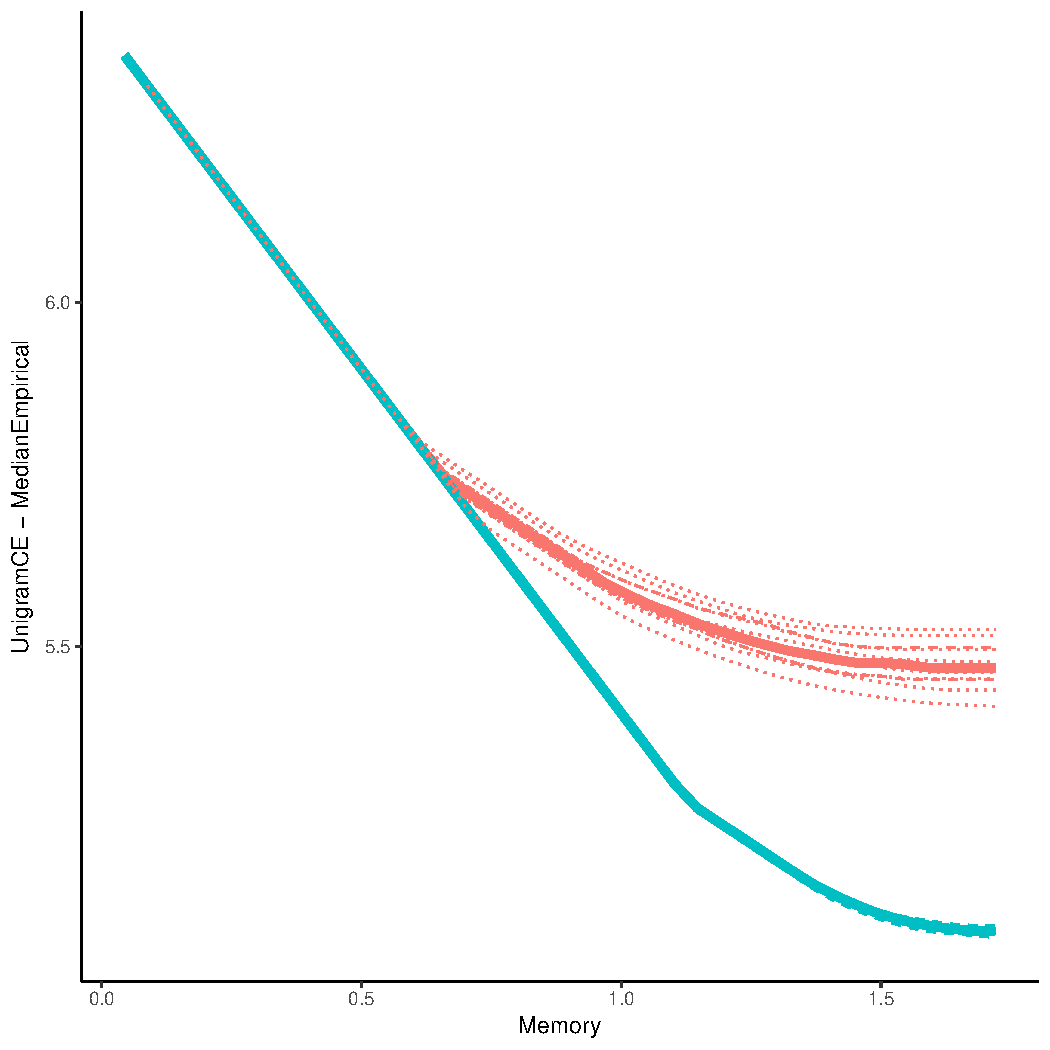
\includegraphics[width=0.25\textwidth]{neural/figures/Japanese-listener-surprisal-memory-MEDIANS_QUANTILES_onlyWordForms_boundedVocab_REAL.pdf} & 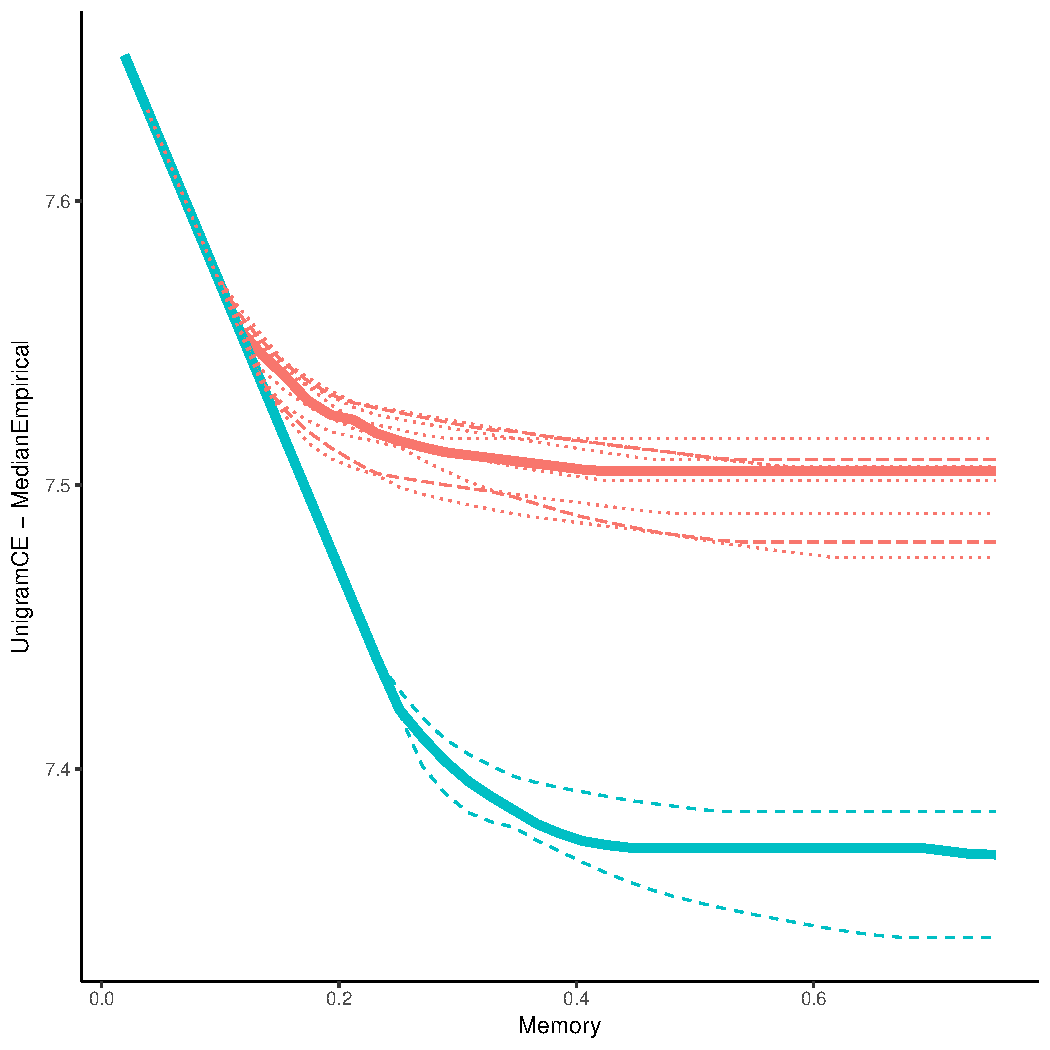
\includegraphics[width=0.25\textwidth]{neural/figures/Kazakh-Adap-listener-surprisal-memory-MEDIANS_QUANTILES_onlyWordForms_boundedVocab_REAL.pdf} & 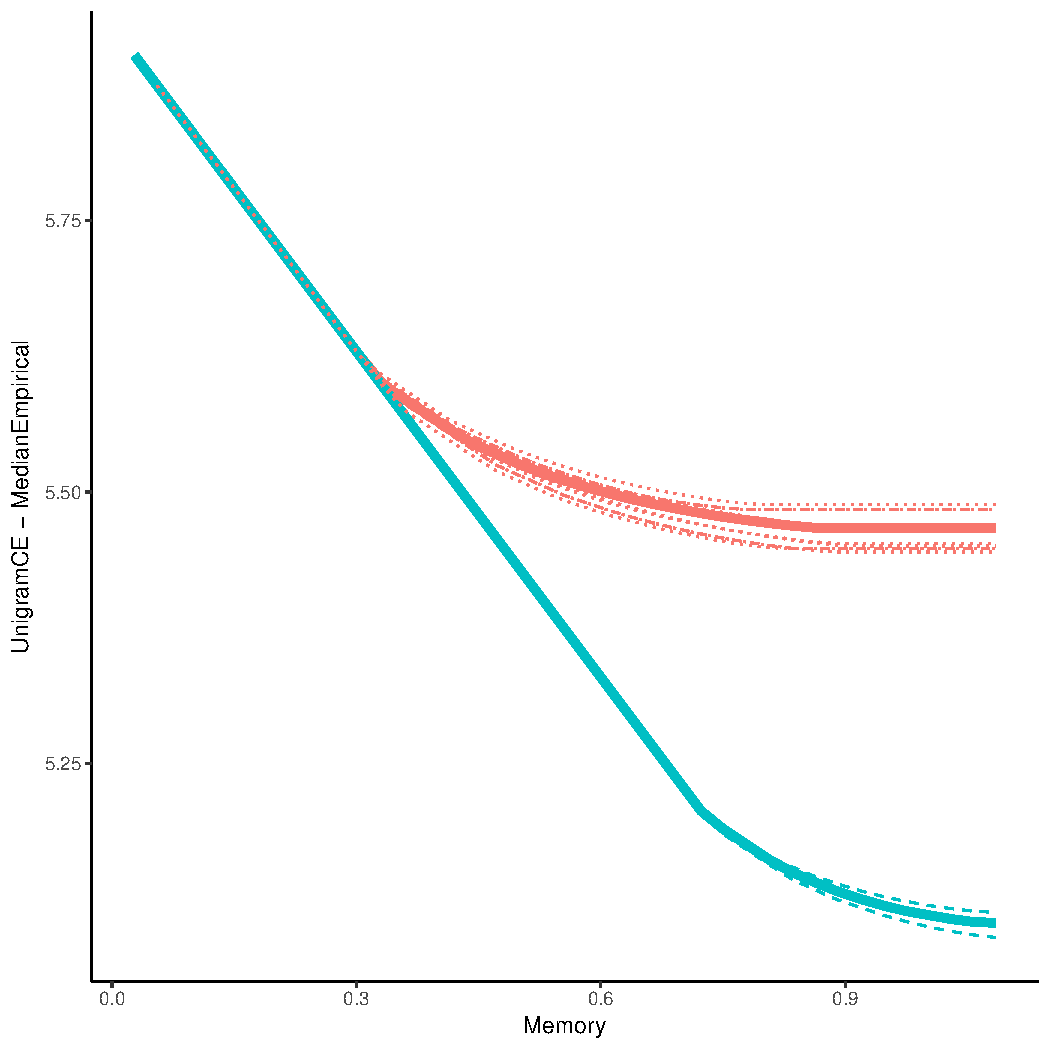
\includegraphics[width=0.25\textwidth]{neural/figures/Korean-listener-surprisal-memory-MEDIANS_QUANTILES_onlyWordForms_boundedVocab_REAL.pdf}
 \\ 

\end{longtable}
	\caption{Medians (cont.)}
\end{table}

\begin{table}
\begin{longtable}{ccccccccccccccclll}
Kurmanji & Latvian & Maltese & Naija
 \\ 
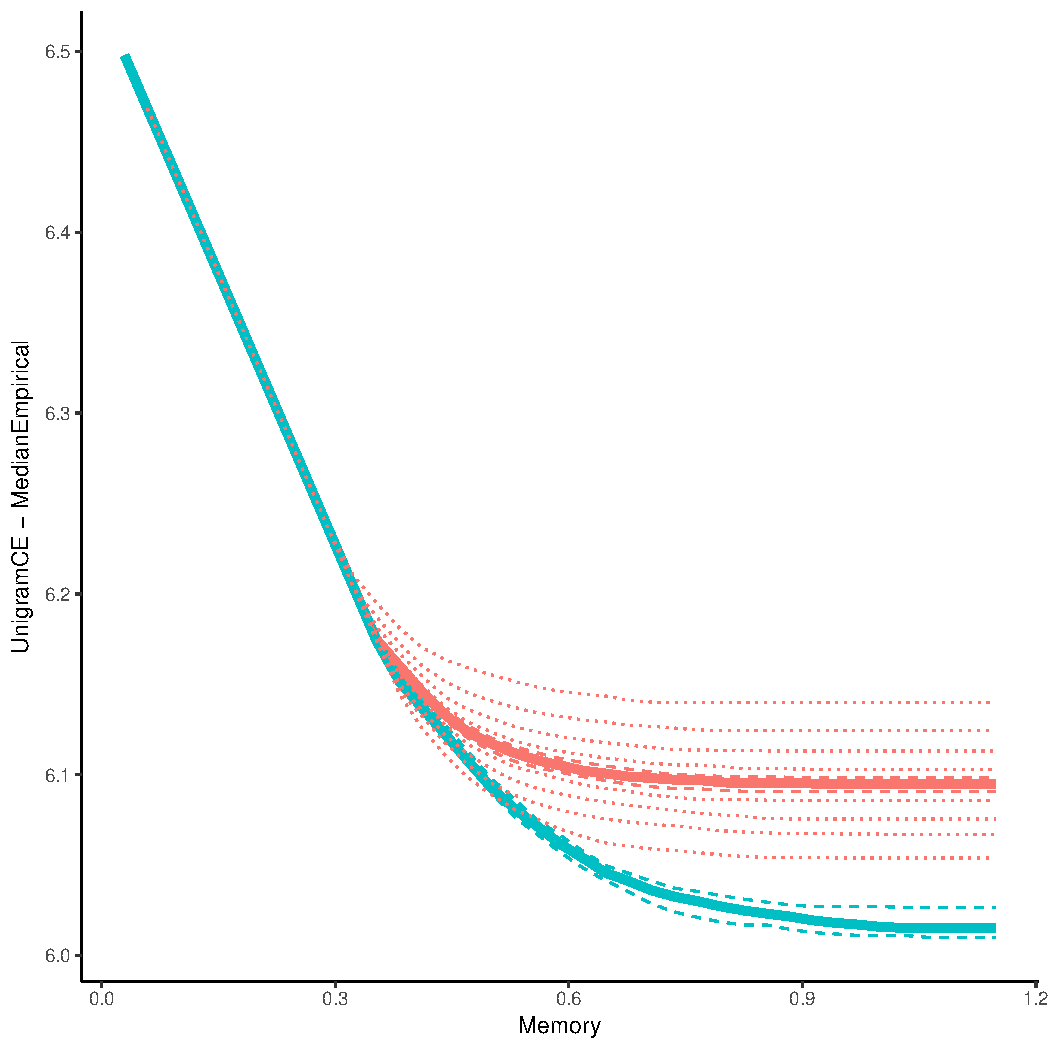
\includegraphics[width=0.25\textwidth]{neural/figures/Kurmanji-Adap-listener-surprisal-memory-MEDIANS_QUANTILES_onlyWordForms_boundedVocab_REAL.pdf} & 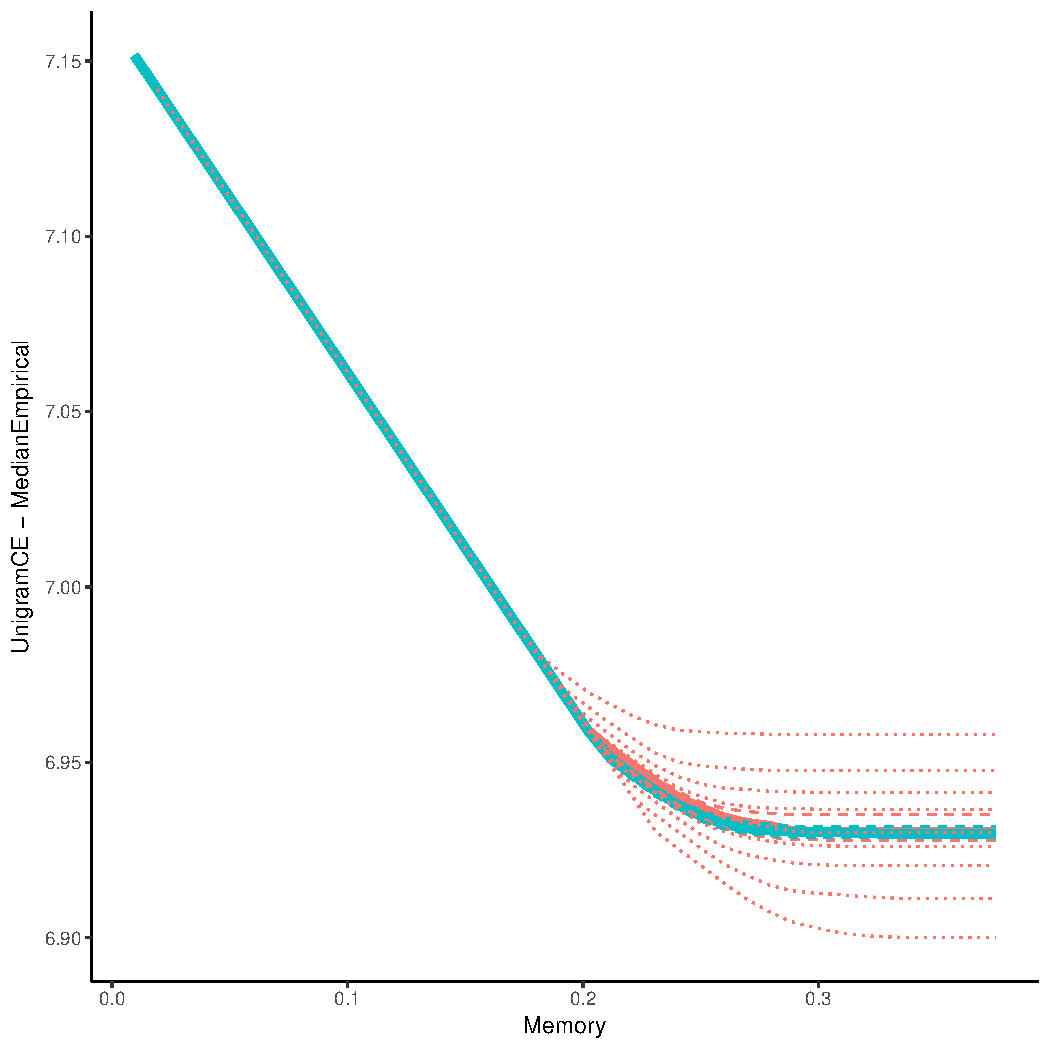
\includegraphics[width=0.25\textwidth]{neural/figures/Latvian-listener-surprisal-memory-MEDIANS_QUANTILES_onlyWordForms_boundedVocab_REAL.pdf} & \includegraphics[width=0.25\textwidth]{neural/figures/Maltese-listener-surprisal-memory-MEDIANS_QUANTILES_onlyWordForms_boundedVocab_REAL.pdf} & \includegraphics[width=0.25\textwidth]{neural/figures/Naija-Adap-listener-surprisal-memory-MEDIANS_QUANTILES_onlyWordForms_boundedVocab_REAL.pdf}
 \\ 
North Sami & Norwegian & Persian & Polish
 \\ 
\includegraphics[width=0.25\textwidth]{neural/figures/North_Sami-listener-surprisal-memory-MEDIANS_QUANTILES_onlyWordForms_boundedVocab_REAL.pdf} & \includegraphics[width=0.25\textwidth]{neural/figures/Norwegian-listener-surprisal-memory-MEDIANS_QUANTILES_onlyWordForms_boundedVocab_REAL.pdf} & \includegraphics[width=0.25\textwidth]{neural/figures/Persian-listener-surprisal-memory-MEDIANS_QUANTILES_onlyWordForms_boundedVocab_REAL.pdf} & \includegraphics[width=0.25\textwidth]{neural/figures/Polish-listener-surprisal-memory-MEDIANS_QUANTILES_onlyWordForms_boundedVocab_REAL.pdf}
 \\ 
Portuguese & Romanian & Russian & Serbian
 \\ 
\includegraphics[width=0.25\textwidth]{neural/figures/Portuguese-listener-surprisal-memory-MEDIANS_QUANTILES_onlyWordForms_boundedVocab_REAL.pdf} & \includegraphics[width=0.25\textwidth]{neural/figures/Romanian-listener-surprisal-memory-MEDIANS_QUANTILES_onlyWordForms_boundedVocab_REAL.pdf} & \includegraphics[width=0.25\textwidth]{neural/figures/Russian-listener-surprisal-memory-MEDIANS_QUANTILES_onlyWordForms_boundedVocab_REAL.pdf} & \includegraphics[width=0.25\textwidth]{neural/figures/Serbian-listener-surprisal-memory-MEDIANS_QUANTILES_onlyWordForms_boundedVocab_REAL.pdf}
 \\ 
Slovak & Slovenian & Spanish & Swedish
 \\ 
\includegraphics[width=0.25\textwidth]{neural/figures/Slovak-listener-surprisal-memory-MEDIANS_QUANTILES_onlyWordForms_boundedVocab_REAL.pdf} & \includegraphics[width=0.25\textwidth]{neural/figures/Slovenian-listener-surprisal-memory-MEDIANS_QUANTILES_onlyWordForms_boundedVocab_REAL.pdf} & \includegraphics[width=0.25\textwidth]{neural/figures/Spanish-listener-surprisal-memory-MEDIANS_QUANTILES_onlyWordForms_boundedVocab_REAL.pdf} & \includegraphics[width=0.25\textwidth]{neural/figures/Swedish-listener-surprisal-memory-MEDIANS_QUANTILES_onlyWordForms_boundedVocab_REAL.pdf}
 \\ 

\end{longtable}
	\caption{Medians (cont.)}
\end{table}

\begin{table}
\begin{longtable}{ccccccccccccccclll}
Thai & Turkish & Ukrainian & Urdu
 \\ 
\includegraphics[width=0.25\textwidth]{neural/figures/Thai-Adap-listener-surprisal-memory-MEDIANS_onlyWordForms_boundedVocab_REAL.pdf} & \includegraphics[width=0.25\textwidth]{neural/figures/Turkish-listener-surprisal-memory-MEDIANS_onlyWordForms_boundedVocab_REAL.pdf} & \includegraphics[width=0.25\textwidth]{neural/figures/Ukrainian-listener-surprisal-memory-MEDIANS_onlyWordForms_boundedVocab_REAL.pdf} & \includegraphics[width=0.25\textwidth]{neural/figures/Urdu-listener-surprisal-memory-MEDIANS_onlyWordForms_boundedVocab_REAL.pdf}
 \\ 
Uyghur & Vietnamese &  & 
 \\ 
\includegraphics[width=0.25\textwidth]{neural/figures/Uyghur-Adap-listener-surprisal-memory-MEDIANS_onlyWordForms_boundedVocab_REAL.pdf} & \includegraphics[width=0.25\textwidth]{neural/figures/Vietnamese-listener-surprisal-memory-MEDIANS_onlyWordForms_boundedVocab_REAL.pdf} &  & 
 \\ 

\end{longtable}
	\caption{Medians (cont.)}
\end{table}







\begin{table}
\begin{longtable}{ccccccccccccccclll}
Afrikaans & Amharic & Arabic & Armenian
 \\ 
\includegraphics[width=0.25\textwidth]{neural/figures/Afrikaans-listener-surprisal-memory-HIST_byMem_onlyWordForms_boundedVocab_REAL.pdf} & \includegraphics[width=0.25\textwidth]{neural/figures/Amharic-Adap-listener-surprisal-memory-HIST_byMem_onlyWordForms_boundedVocab_REAL.pdf} & \includegraphics[width=0.25\textwidth]{neural/figures/Arabic-listener-surprisal-memory-HIST_byMem_onlyWordForms_boundedVocab_REAL.pdf} & \includegraphics[width=0.25\textwidth]{neural/figures/Armenian-Adap-listener-surprisal-memory-HIST_byMem_onlyWordForms_boundedVocab_REAL.pdf}
 \\ 
Bambara & Basque & Breton & Bulgarian
 \\ 
\includegraphics[width=0.25\textwidth]{neural/figures/Bambara-Adap-listener-surprisal-memory-HIST_byMem_onlyWordForms_boundedVocab_REAL.pdf} & \includegraphics[width=0.25\textwidth]{neural/figures/Basque-listener-surprisal-memory-HIST_byMem_onlyWordForms_boundedVocab_REAL.pdf} & \includegraphics[width=0.25\textwidth]{neural/figures/Breton-Adap-listener-surprisal-memory-HIST_byMem_onlyWordForms_boundedVocab_REAL.pdf} & \includegraphics[width=0.25\textwidth]{neural/figures/Bulgarian-listener-surprisal-memory-HIST_byMem_onlyWordForms_boundedVocab_REAL.pdf}
 \\ 
Buryat & Cantonese & Catalan & Chinese
 \\ 
\includegraphics[width=0.25\textwidth]{neural/figures/Buryat-Adap-listener-surprisal-memory-HIST_byMem_onlyWordForms_boundedVocab_REAL.pdf} & \includegraphics[width=0.25\textwidth]{neural/figures/Cantonese-Adap-listener-surprisal-memory-HIST_byMem_onlyWordForms_boundedVocab_REAL.pdf} & \includegraphics[width=0.25\textwidth]{neural/figures/Catalan-listener-surprisal-memory-HIST_byMem_onlyWordForms_boundedVocab_REAL.pdf} & \includegraphics[width=0.25\textwidth]{neural/figures/Chinese-listener-surprisal-memory-HIST_byMem_onlyWordForms_boundedVocab_REAL.pdf}
 \\ 
Croatian & Czech & Danish & Dutch
 \\ 
\includegraphics[width=0.25\textwidth]{neural/figures/Croatian-listener-surprisal-memory-HIST_byMem_onlyWordForms_boundedVocab_REAL.pdf} & \includegraphics[width=0.25\textwidth]{neural/figures/Czech-listener-surprisal-memory-HIST_byMem_onlyWordForms_boundedVocab_REAL.pdf} & \includegraphics[width=0.25\textwidth]{neural/figures/Danish-listener-surprisal-memory-HIST_byMem_onlyWordForms_boundedVocab_REAL.pdf} & \includegraphics[width=0.25\textwidth]{neural/figures/Dutch-listener-surprisal-memory-HIST_byMem_onlyWordForms_boundedVocab_REAL.pdf}
 \\ 

\end{longtable}
	\caption{Histograms: Surprisal, at maximum memory.}\label{tab:slice-hists-real}
\end{table}

\begin{table}
\begin{longtable}{ccccccccccccccclll}
English & Erzya & Estonian & Faroese
 \\ 
\includegraphics[width=0.25\textwidth]{neural/figures/English-listener-surprisal-memory-HIST_byMem_onlyWordForms_boundedVocab_REAL.pdf} & \includegraphics[width=0.25\textwidth]{neural/figures/Erzya-Adap-listener-surprisal-memory-HIST_byMem_onlyWordForms_boundedVocab_REAL.pdf} & \includegraphics[width=0.25\textwidth]{neural/figures/Estonian-listener-surprisal-memory-HIST_byMem_onlyWordForms_boundedVocab_REAL.pdf} & \includegraphics[width=0.25\textwidth]{neural/figures/Faroese-Adap-listener-surprisal-memory-HIST_byMem_onlyWordForms_boundedVocab_REAL.pdf}
 \\ 
Finnish & French & German & Greek
 \\ 
\includegraphics[width=0.25\textwidth]{neural/figures/Finnish-listener-surprisal-memory-HIST_byMem_onlyWordForms_boundedVocab_REAL.pdf} & \includegraphics[width=0.25\textwidth]{neural/figures/French-listener-surprisal-memory-HIST_byMem_onlyWordForms_boundedVocab_REAL.pdf} & \includegraphics[width=0.25\textwidth]{neural/figures/German-listener-surprisal-memory-HIST_byMem_onlyWordForms_boundedVocab_REAL.pdf} & \includegraphics[width=0.25\textwidth]{neural/figures/Greek-listener-surprisal-memory-HIST_byMem_onlyWordForms_boundedVocab_REAL.pdf}
 \\ 
Hebrew & Hindi & Hungarian & Indonesian
 \\ 
\includegraphics[width=0.25\textwidth]{neural/figures/Hebrew-listener-surprisal-memory-HIST_byMem_onlyWordForms_boundedVocab_REAL.pdf} & \includegraphics[width=0.25\textwidth]{neural/figures/Hindi-listener-surprisal-memory-HIST_byMem_onlyWordForms_boundedVocab_REAL.pdf} & \includegraphics[width=0.25\textwidth]{neural/figures/Hungarian-listener-surprisal-memory-HIST_byMem_onlyWordForms_boundedVocab_REAL.pdf} & \includegraphics[width=0.25\textwidth]{neural/figures/Indonesian-listener-surprisal-memory-HIST_byMem_onlyWordForms_boundedVocab_REAL.pdf}
 \\ 
Italian & Japanese & Kazakh & Korean
 \\ 
\includegraphics[width=0.25\textwidth]{neural/figures/Italian-listener-surprisal-memory-HIST_byMem_onlyWordForms_boundedVocab_REAL.pdf} & \includegraphics[width=0.25\textwidth]{neural/figures/Japanese-listener-surprisal-memory-HIST_byMem_onlyWordForms_boundedVocab_REAL.pdf} & \includegraphics[width=0.25\textwidth]{neural/figures/Kazakh-Adap-listener-surprisal-memory-HIST_byMem_onlyWordForms_boundedVocab_REAL.pdf} & \includegraphics[width=0.25\textwidth]{neural/figures/Korean-listener-surprisal-memory-HIST_byMem_onlyWordForms_boundedVocab_REAL.pdf}
 \\ 

\end{longtable}
	\caption{Medians (cont.)}
\end{table}

\begin{table}
\begin{longtable}{ccccccccccccccclll}
Kurmanji & Latvian & Maltese & Naija
 \\ 
\includegraphics[width=0.25\textwidth]{neural/figures/Kurmanji-Adap-listener-surprisal-memory-HIST_byMem_onlyWordForms_boundedVocab_REAL.pdf} & \includegraphics[width=0.25\textwidth]{neural/figures/Latvian-listener-surprisal-memory-HIST_byMem_onlyWordForms_boundedVocab_REAL.pdf} & \includegraphics[width=0.25\textwidth]{neural/figures/Maltese-listener-surprisal-memory-HIST_byMem_onlyWordForms_boundedVocab_REAL.pdf} & \includegraphics[width=0.25\textwidth]{neural/figures/Naija-Adap-listener-surprisal-memory-HIST_byMem_onlyWordForms_boundedVocab_REAL.pdf}
 \\ 
North Sami & Norwegian & Persian & Polish
 \\ 
\includegraphics[width=0.25\textwidth]{neural/figures/North_Sami-listener-surprisal-memory-HIST_byMem_onlyWordForms_boundedVocab_REAL.pdf} & \includegraphics[width=0.25\textwidth]{neural/figures/Norwegian-listener-surprisal-memory-HIST_byMem_onlyWordForms_boundedVocab_REAL.pdf} & \includegraphics[width=0.25\textwidth]{neural/figures/Persian-listener-surprisal-memory-HIST_byMem_onlyWordForms_boundedVocab_REAL.pdf} & \includegraphics[width=0.25\textwidth]{neural/figures/Polish-listener-surprisal-memory-HIST_byMem_onlyWordForms_boundedVocab_REAL.pdf}
 \\ 
Portuguese & Romanian & Russian & Serbian
 \\ 
\includegraphics[width=0.25\textwidth]{neural/figures/Portuguese-listener-surprisal-memory-HIST_byMem_onlyWordForms_boundedVocab_REAL.pdf} & \includegraphics[width=0.25\textwidth]{neural/figures/Romanian-listener-surprisal-memory-HIST_byMem_onlyWordForms_boundedVocab_REAL.pdf} & \includegraphics[width=0.25\textwidth]{neural/figures/Russian-listener-surprisal-memory-HIST_byMem_onlyWordForms_boundedVocab_REAL.pdf} & \includegraphics[width=0.25\textwidth]{neural/figures/Serbian-listener-surprisal-memory-HIST_byMem_onlyWordForms_boundedVocab_REAL.pdf}
 \\ 
Slovak & Slovenian & Spanish & Swedish
 \\ 
\includegraphics[width=0.25\textwidth]{neural/figures/Slovak-listener-surprisal-memory-HIST_byMem_onlyWordForms_boundedVocab_REAL.pdf} & \includegraphics[width=0.25\textwidth]{neural/figures/Slovenian-listener-surprisal-memory-HIST_byMem_onlyWordForms_boundedVocab_REAL.pdf} & \includegraphics[width=0.25\textwidth]{neural/figures/Spanish-listener-surprisal-memory-HIST_byMem_onlyWordForms_boundedVocab_REAL.pdf} & \includegraphics[width=0.25\textwidth]{neural/figures/Swedish-listener-surprisal-memory-HIST_byMem_onlyWordForms_boundedVocab_REAL.pdf}
 \\ 

\end{longtable}
	\caption{Medians (cont.)}
\end{table}

\begin{table}
\begin{longtable}{ccccccccccccccclll}
Thai & Turkish & Ukrainian & Urdu
 \\ 
\includegraphics[width=0.25\textwidth]{neural/figures/Thai-Adap-listener-surprisal-memory-HIST_byMem_onlyWordForms_boundedVocab_REAL.pdf} & \includegraphics[width=0.25\textwidth]{neural/figures/Turkish-listener-surprisal-memory-HIST_byMem_onlyWordForms_boundedVocab_REAL.pdf} & \includegraphics[width=0.25\textwidth]{neural/figures/Ukrainian-listener-surprisal-memory-HIST_byMem_onlyWordForms_boundedVocab_REAL.pdf} & \includegraphics[width=0.25\textwidth]{neural/figures/Urdu-listener-surprisal-memory-HIST_byMem_onlyWordForms_boundedVocab_REAL.pdf}
 \\ 
Uyghur & Vietnamese &  & 
 \\ 
\includegraphics[width=0.25\textwidth]{neural/figures/Uyghur-Adap-listener-surprisal-memory-HIST_byMem_onlyWordForms_boundedVocab_REAL.pdf} & \includegraphics[width=0.25\textwidth]{neural/figures/Vietnamese-listener-surprisal-memory-HIST_byMem_onlyWordForms_boundedVocab_REAL.pdf} &  & 
 \\ 

\end{longtable}
	\caption{Medians (cont.)}
\end{table}


\begin{table}
\begin{longtable}{cccccccccccccccccc}
Afrikaans & Amharic & Arabic & Armenian
 \\ 
\includegraphics[width=0.25\textwidth]{neural/figures/Afrikaans-listener-surprisal-memory-QUANTILES_onlyWordForms_boundedVocab_REAL.pdf} & \includegraphics[width=0.25\textwidth]{neural/figures/Amharic-Adap-listener-surprisal-memory-QUANTILES_onlyWordForms_boundedVocab_REAL.pdf} & \includegraphics[width=0.25\textwidth]{neural/figures/Arabic-listener-surprisal-memory-QUANTILES_onlyWordForms_boundedVocab_REAL.pdf} & \includegraphics[width=0.25\textwidth]{neural/figures/Armenian-Adap-listener-surprisal-memory-QUANTILES_onlyWordForms_boundedVocab_REAL.pdf}
 \\ 
Bambara & Basque & Breton & Bulgarian
 \\ 
\includegraphics[width=0.25\textwidth]{neural/figures/Bambara-Adap-listener-surprisal-memory-QUANTILES_onlyWordForms_boundedVocab_REAL.pdf} & \includegraphics[width=0.25\textwidth]{neural/figures/Basque-listener-surprisal-memory-QUANTILES_onlyWordForms_boundedVocab_REAL.pdf} & \includegraphics[width=0.25\textwidth]{neural/figures/Breton-Adap-listener-surprisal-memory-QUANTILES_onlyWordForms_boundedVocab_REAL.pdf} & \includegraphics[width=0.25\textwidth]{neural/figures/Bulgarian-listener-surprisal-memory-QUANTILES_onlyWordForms_boundedVocab_REAL.pdf}
 \\ 
Buryat & Cantonese & Catalan & Chinese
 \\ 
\includegraphics[width=0.25\textwidth]{neural/figures/Buryat-Adap-listener-surprisal-memory-QUANTILES_onlyWordForms_boundedVocab_REAL.pdf} & \includegraphics[width=0.25\textwidth]{neural/figures/Cantonese-Adap-listener-surprisal-memory-QUANTILES_onlyWordForms_boundedVocab_REAL.pdf} & \includegraphics[width=0.25\textwidth]{neural/figures/Catalan-listener-surprisal-memory-QUANTILES_onlyWordForms_boundedVocab_REAL.pdf} & \includegraphics[width=0.25\textwidth]{neural/figures/Chinese-listener-surprisal-memory-QUANTILES_onlyWordForms_boundedVocab_REAL.pdf}
 \\ 
Croatian & Czech & Danish & Dutch
 \\ 
\includegraphics[width=0.25\textwidth]{neural/figures/Croatian-listener-surprisal-memory-QUANTILES_onlyWordForms_boundedVocab_REAL.pdf} & \includegraphics[width=0.25\textwidth]{neural/figures/Czech-listener-surprisal-memory-QUANTILES_onlyWordForms_boundedVocab_REAL.pdf} & \includegraphics[width=0.25\textwidth]{neural/figures/Danish-listener-surprisal-memory-QUANTILES_onlyWordForms_boundedVocab_REAL.pdf} & \includegraphics[width=0.25\textwidth]{neural/figures/Dutch-listener-surprisal-memory-QUANTILES_onlyWordForms_boundedVocab_REAL.pdf}
 \\ 
English & Erzya & Estonian & Faroese
 \\ 
\includegraphics[width=0.25\textwidth]{neural/figures/English-listener-surprisal-memory-QUANTILES_onlyWordForms_boundedVocab_REAL.pdf} & \includegraphics[width=0.25\textwidth]{neural/figures/Erzya-Adap-listener-surprisal-memory-QUANTILES_onlyWordForms_boundedVocab_REAL.pdf} & \includegraphics[width=0.25\textwidth]{neural/figures/Estonian-listener-surprisal-memory-QUANTILES_onlyWordForms_boundedVocab_REAL.pdf} & \includegraphics[width=0.25\textwidth]{neural/figures/Faroese-Adap-listener-surprisal-memory-QUANTILES_onlyWordForms_boundedVocab_REAL.pdf}
 \\ 

\end{longtable}
	\caption{Quantiles: At a given memory budget, what percentage of the baselines results in higher listener surprisal than the real language? Solid curves represent sample means, dashed lines represent 95 \% confidence bounds; dotted lines represent 99.9 \% confidence bounds. At five evenly spaced memory levels, we provide a p-value for the null hypothesis that the actual population mean is $0.5$ or less. Confidence bounds and p-values are obtained using an exact nonparametric method (see text).}\label{tab:quantiles}
\end{table}

\begin{table}
\begin{longtable}{cccccccccccccccccc}
Finnish & French & German & Greek
 \\ 
\includegraphics[width=0.25\textwidth]{neural/figures/Finnish-listener-surprisal-memory-QUANTILES_onlyWordForms_boundedVocab_REAL.pdf} & \includegraphics[width=0.25\textwidth]{neural/figures/French-listener-surprisal-memory-QUANTILES_onlyWordForms_boundedVocab_REAL.pdf} & \includegraphics[width=0.25\textwidth]{neural/figures/German-listener-surprisal-memory-QUANTILES_onlyWordForms_boundedVocab_REAL.pdf} & \includegraphics[width=0.25\textwidth]{neural/figures/Greek-listener-surprisal-memory-QUANTILES_onlyWordForms_boundedVocab_REAL.pdf}
 \\ 
Hebrew & Hindi & Hungarian & Indonesian
 \\ 
\includegraphics[width=0.25\textwidth]{neural/figures/Hebrew-listener-surprisal-memory-QUANTILES_onlyWordForms_boundedVocab_REAL.pdf} & \includegraphics[width=0.25\textwidth]{neural/figures/Hindi-listener-surprisal-memory-QUANTILES_onlyWordForms_boundedVocab_REAL.pdf} & \includegraphics[width=0.25\textwidth]{neural/figures/Hungarian-listener-surprisal-memory-QUANTILES_onlyWordForms_boundedVocab_REAL.pdf} & \includegraphics[width=0.25\textwidth]{neural/figures/Indonesian-listener-surprisal-memory-QUANTILES_onlyWordForms_boundedVocab_REAL.pdf}
 \\ 
Italian & Japanese & Kazakh & Korean
 \\ 
\includegraphics[width=0.25\textwidth]{neural/figures/Italian-listener-surprisal-memory-QUANTILES_onlyWordForms_boundedVocab_REAL.pdf} & \includegraphics[width=0.25\textwidth]{neural/figures/Japanese-listener-surprisal-memory-QUANTILES_onlyWordForms_boundedVocab_REAL.pdf} & \includegraphics[width=0.25\textwidth]{neural/figures/Kazakh-Adap-listener-surprisal-memory-QUANTILES_onlyWordForms_boundedVocab_REAL.pdf} & \includegraphics[width=0.25\textwidth]{neural/figures/Korean-listener-surprisal-memory-QUANTILES_onlyWordForms_boundedVocab_REAL.pdf}
 \\ 
Kurmanji & Latvian & Maltese & Naija
 \\ 
\includegraphics[width=0.25\textwidth]{neural/figures/Kurmanji-Adap-listener-surprisal-memory-QUANTILES_onlyWordForms_boundedVocab_REAL.pdf} & \includegraphics[width=0.25\textwidth]{neural/figures/Latvian-listener-surprisal-memory-QUANTILES_onlyWordForms_boundedVocab_REAL.pdf} & \includegraphics[width=0.25\textwidth]{neural/figures/Maltese-listener-surprisal-memory-QUANTILES_onlyWordForms_boundedVocab_REAL.pdf} & \includegraphics[width=0.25\textwidth]{neural/figures/Naija-Adap-listener-surprisal-memory-QUANTILES_onlyWordForms_boundedVocab_REAL.pdf}
 \\ 
North Sami & Norwegian & Persian & Polish
 \\ 
\includegraphics[width=0.25\textwidth]{neural/figures/North_Sami-listener-surprisal-memory-QUANTILES_onlyWordForms_boundedVocab_REAL.pdf} & \includegraphics[width=0.25\textwidth]{neural/figures/Norwegian-listener-surprisal-memory-QUANTILES_onlyWordForms_boundedVocab_REAL.pdf} & \includegraphics[width=0.25\textwidth]{neural/figures/Persian-listener-surprisal-memory-QUANTILES_onlyWordForms_boundedVocab_REAL.pdf} & \includegraphics[width=0.25\textwidth]{neural/figures/Polish-listener-surprisal-memory-QUANTILES_onlyWordForms_boundedVocab_REAL.pdf}
 \\ 

\end{longtable}
	\caption{Quantiles (part 2)}
\end{table}

\begin{table}
\begin{longtable}{cccccccccccccccccc}
Portuguese & Romanian & Russian & Serbian
 \\ 
\includegraphics[width=0.25\textwidth]{neural/figures/Portuguese-listener-surprisal-memory-QUANTILES_onlyWordForms_boundedVocab_REAL.pdf} & \includegraphics[width=0.25\textwidth]{neural/figures/Romanian-listener-surprisal-memory-QUANTILES_onlyWordForms_boundedVocab_REAL.pdf} & \includegraphics[width=0.25\textwidth]{neural/figures/Russian-listener-surprisal-memory-QUANTILES_onlyWordForms_boundedVocab_REAL.pdf} & \includegraphics[width=0.25\textwidth]{neural/figures/Serbian-listener-surprisal-memory-QUANTILES_onlyWordForms_boundedVocab_REAL.pdf}
 \\ 
Slovak & Slovenian & Spanish & Swedish
 \\ 
\includegraphics[width=0.25\textwidth]{neural/figures/Slovak-listener-surprisal-memory-QUANTILES_onlyWordForms_boundedVocab_REAL.pdf} & \includegraphics[width=0.25\textwidth]{neural/figures/Slovenian-listener-surprisal-memory-QUANTILES_onlyWordForms_boundedVocab_REAL.pdf} & \includegraphics[width=0.25\textwidth]{neural/figures/Spanish-listener-surprisal-memory-QUANTILES_onlyWordForms_boundedVocab_REAL.pdf} & \includegraphics[width=0.25\textwidth]{neural/figures/Swedish-listener-surprisal-memory-QUANTILES_onlyWordForms_boundedVocab_REAL.pdf}
 \\ 
Thai & Turkish & Ukrainian & Urdu
 \\ 
\includegraphics[width=0.25\textwidth]{neural/figures/Thai-Adap-listener-surprisal-memory-QUANTILES_onlyWordForms_boundedVocab_REAL.pdf} & \includegraphics[width=0.25\textwidth]{neural/figures/Turkish-listener-surprisal-memory-QUANTILES_onlyWordForms_boundedVocab_REAL.pdf} & \includegraphics[width=0.25\textwidth]{neural/figures/Ukrainian-listener-surprisal-memory-QUANTILES_onlyWordForms_boundedVocab_REAL.pdf} & \includegraphics[width=0.25\textwidth]{neural/figures/Urdu-listener-surprisal-memory-QUANTILES_onlyWordForms_boundedVocab_REAL.pdf}
 \\ 
Uyghur & Vietnamese &  & 
 \\ 
\includegraphics[width=0.25\textwidth]{neural/figures/Uyghur-Adap-listener-surprisal-memory-QUANTILES_onlyWordForms_boundedVocab_REAL.pdf} & \includegraphics[width=0.25\textwidth]{neural/figures/Vietnamese-listener-surprisal-memory-QUANTILES_onlyWordForms_boundedVocab_REAL.pdf} &  & 
 \\ 

\end{longtable}
	\caption{Quantiles (part 3)}
\end{table}





















\begin{table}
\begin{longtable}{l|ll||l|llllllllllllll}
	Language & Base. & MLE & Language & Base. & MLE \\ \hline
Afrikaans  &  13  &  10  &  Indonesian  &  11  &  10  \\
Amharic  &  137  &  71  &  Italian  &  10  &  10  \\
Arabic  &  11  &  10  &  Japanese  &  25  &  10  \\
Armenian  &  140  &  17  &  Kazakh  &  11  &  10  \\
Bambara  &  25  &  10  &  Korean  &  11  &  10  \\
Basque  &  15  &  10  &  Kurmanji  &  338  &  101  \\
Breton  &  35  &  10  &  Latvian  &  308  &  132  \\
Bulgarian  &  14  &  10  &  Maltese  &  30  &  10  \\
Buryat  &  26  &  10  &  Naija  &  214  &  93  \\
Cantonese  &  306  &  135  &  North Sami  &  335  &  101  \\
Catalan  &  11  &  10  &  Norwegian  &  12  &  10  \\
Chinese  &  21  &  10  &  Persian  &  25  &  10  \\
Croatian  &  30  &  10  &  Polish  &  309  &  131  \\
Czech  &  18  &  12  &  Portuguese  &  15  &  99  \\
Danish  &  33  &  10  &  Romanian  &  10  &  10  \\
Dutch  &  27  &  10  &  Russian  &  20  &  13  \\
English  &  13  &  10  &  Serbian  &  26  &  11  \\
Erzya  &  846  &  101  &  Slovak  &  303  &  138  \\
Estonian  &  347  &  10  &  Slovenian  &  297  &  12  \\
Faroese  &  27  &  10  &  Spanish  &  14  &  10  \\
Finnish  &  83  &  54  &  Swedish  &  31  &  10  \\
French  &  14  &  12  &  Thai  &  45  &  10  \\
German  &  19  &  10  &  Turkish  &  13  &  10  \\
Greek  &  16  &  10  &  Ukrainian  &  28  &  10  \\
Hebrew  &  11  &  10  &  Urdu  &  17  &  10  \\
Hindi  &  11  &  10  &  Uyghur  &  326  &  132  \\
Hungarian  &  220  &  35  &  Vietnamese  &  303  &  132  \\

\end{longtable}
	\caption{Experiment 3: Samples drawn per language according to the precision-dependent stopping criterion.}\label{tab:samples}
\end{table}





\begin{table}
\begin{longtable}{ccccccccccccccclll}
Afrikaans & Amharic & Arabic & Armenian
 \\ 
\includegraphics[width=0.25\textwidth]{neural/figures/Afrikaans-listener-surprisal-memory-MEDIANS_QUANTILES_onlyWordForms_boundedVocab.pdf} & \includegraphics[width=0.25\textwidth]{neural/figures/Amharic-Adap-listener-surprisal-memory-MEDIANS_QUANTILES_onlyWordForms_boundedVocab.pdf} & \includegraphics[width=0.25\textwidth]{neural/figures/Arabic-listener-surprisal-memory-MEDIANS_QUANTILES_onlyWordForms_boundedVocab.pdf} & \includegraphics[width=0.25\textwidth]{neural/figures/Armenian-Adap-listener-surprisal-memory-MEDIANS_QUANTILES_onlyWordForms_boundedVocab.pdf}
 \\ 
Bambara & Basque & Breton & Bulgarian
 \\ 
\includegraphics[width=0.25\textwidth]{neural/figures/Bambara-Adap-listener-surprisal-memory-MEDIANS_QUANTILES_onlyWordForms_boundedVocab.pdf} & \includegraphics[width=0.25\textwidth]{neural/figures/Basque-listener-surprisal-memory-MEDIANS_QUANTILES_onlyWordForms_boundedVocab.pdf} & \includegraphics[width=0.25\textwidth]{neural/figures/Breton-Adap-listener-surprisal-memory-MEDIANS_QUANTILES_onlyWordForms_boundedVocab.pdf} & \includegraphics[width=0.25\textwidth]{neural/figures/Bulgarian-listener-surprisal-memory-MEDIANS_QUANTILES_onlyWordForms_boundedVocab.pdf}
 \\ 
Buryat & Cantonese & Catalan & Chinese
 \\ 
\includegraphics[width=0.25\textwidth]{neural/figures/Buryat-Adap-listener-surprisal-memory-MEDIANS_QUANTILES_onlyWordForms_boundedVocab.pdf} & \includegraphics[width=0.25\textwidth]{neural/figures/Cantonese-Adap-listener-surprisal-memory-MEDIANS_QUANTILES_onlyWordForms_boundedVocab.pdf} & \includegraphics[width=0.25\textwidth]{neural/figures/Catalan-listener-surprisal-memory-MEDIANS_QUANTILES_onlyWordForms_boundedVocab.pdf} & \includegraphics[width=0.25\textwidth]{neural/figures/Chinese-listener-surprisal-memory-MEDIANS_QUANTILES_onlyWordForms_boundedVocab.pdf}
 \\ 
Croatian & Czech & Danish & Dutch
 \\ 
\includegraphics[width=0.25\textwidth]{neural/figures/Croatian-listener-surprisal-memory-MEDIANS_QUANTILES_onlyWordForms_boundedVocab.pdf} & \includegraphics[width=0.25\textwidth]{neural/figures/Czech-listener-surprisal-memory-MEDIANS_QUANTILES_onlyWordForms_boundedVocab.pdf} & \includegraphics[width=0.25\textwidth]{neural/figures/Danish-listener-surprisal-memory-MEDIANS_QUANTILES_onlyWordForms_boundedVocab.pdf} & \includegraphics[width=0.25\textwidth]{neural/figures/Dutch-listener-surprisal-memory-MEDIANS_QUANTILES_onlyWordForms_boundedVocab.pdf}
 \\ 

\end{longtable}
	\caption{Experiment 3. Medians: For each memory budget, we provide the median surprisal for real and random languages. Solid lines indicate sample medians, dashed lines indicate 95 $\%$ confidence intervals for the population median. Green: Random baselines; blue: real language; red: maximum-likelihood grammars fit to real orderings.}\label{tab:medians}
\end{table}

\begin{table}
\begin{longtable}{ccccccccccccccclll}
English & Erzya & Estonian & Faroese
 \\ 
\includegraphics[width=0.25\textwidth]{neural/figures/English-listener-surprisal-memory-MEDIANS_onlyWordForms_boundedVocab.pdf} & \includegraphics[width=0.25\textwidth]{neural/figures/Erzya-Adap-listener-surprisal-memory-MEDIANS_onlyWordForms_boundedVocab.pdf} & \includegraphics[width=0.25\textwidth]{neural/figures/Estonian-listener-surprisal-memory-MEDIANS_onlyWordForms_boundedVocab.pdf} & \includegraphics[width=0.25\textwidth]{neural/figures/Faroese-Adap-listener-surprisal-memory-MEDIANS_onlyWordForms_boundedVocab.pdf}
 \\ 
Finnish & French & German & Greek
 \\ 
\includegraphics[width=0.25\textwidth]{neural/figures/Finnish-listener-surprisal-memory-MEDIANS_onlyWordForms_boundedVocab.pdf} & \includegraphics[width=0.25\textwidth]{neural/figures/French-listener-surprisal-memory-MEDIANS_onlyWordForms_boundedVocab.pdf} & \includegraphics[width=0.25\textwidth]{neural/figures/German-listener-surprisal-memory-MEDIANS_onlyWordForms_boundedVocab.pdf} & \includegraphics[width=0.25\textwidth]{neural/figures/Greek-listener-surprisal-memory-MEDIANS_onlyWordForms_boundedVocab.pdf}
 \\ 
Hebrew & Hindi & Hungarian & Indonesian
 \\ 
\includegraphics[width=0.25\textwidth]{neural/figures/Hebrew-listener-surprisal-memory-MEDIANS_onlyWordForms_boundedVocab.pdf} & \includegraphics[width=0.25\textwidth]{neural/figures/Hindi-listener-surprisal-memory-MEDIANS_onlyWordForms_boundedVocab.pdf} & \includegraphics[width=0.25\textwidth]{neural/figures/Hungarian-listener-surprisal-memory-MEDIANS_onlyWordForms_boundedVocab.pdf} & \includegraphics[width=0.25\textwidth]{neural/figures/Indonesian-listener-surprisal-memory-MEDIANS_onlyWordForms_boundedVocab.pdf}
 \\ 
Italian & Japanese & Kazakh & Korean
 \\ 
\includegraphics[width=0.25\textwidth]{neural/figures/Italian-listener-surprisal-memory-MEDIANS_onlyWordForms_boundedVocab.pdf} & \includegraphics[width=0.25\textwidth]{neural/figures/Japanese-listener-surprisal-memory-MEDIANS_onlyWordForms_boundedVocab.pdf} & \includegraphics[width=0.25\textwidth]{neural/figures/Kazakh-Adap-listener-surprisal-memory-MEDIANS_onlyWordForms_boundedVocab.pdf} & \includegraphics[width=0.25\textwidth]{neural/figures/Korean-listener-surprisal-memory-MEDIANS_onlyWordForms_boundedVocab.pdf}
 \\ 

\end{longtable}
	\caption{Medians (cont.)}
\end{table}

\begin{table}
\begin{longtable}{ccccccccccccccclll}
Kurmanji & Latvian & Maltese & Naija
 \\ 
\includegraphics[width=0.25\textwidth]{neural/figures/Kurmanji-Adap-listener-surprisal-memory-MEDIANS_onlyWordForms_boundedVocab.pdf} & \includegraphics[width=0.25\textwidth]{neural/figures/Latvian-listener-surprisal-memory-MEDIANS_onlyWordForms_boundedVocab.pdf} & \includegraphics[width=0.25\textwidth]{neural/figures/Maltese-listener-surprisal-memory-MEDIANS_onlyWordForms_boundedVocab.pdf} & \includegraphics[width=0.25\textwidth]{neural/figures/Naija-Adap-listener-surprisal-memory-MEDIANS_onlyWordForms_boundedVocab.pdf}
 \\ 
North Sami & Norwegian & Persian & Polish
 \\ 
\includegraphics[width=0.25\textwidth]{neural/figures/North_Sami-listener-surprisal-memory-MEDIANS_onlyWordForms_boundedVocab.pdf} & \includegraphics[width=0.25\textwidth]{neural/figures/Norwegian-listener-surprisal-memory-MEDIANS_onlyWordForms_boundedVocab.pdf} & \includegraphics[width=0.25\textwidth]{neural/figures/Persian-listener-surprisal-memory-MEDIANS_onlyWordForms_boundedVocab.pdf} & \includegraphics[width=0.25\textwidth]{neural/figures/Polish-listener-surprisal-memory-MEDIANS_onlyWordForms_boundedVocab.pdf}
 \\ 
Portuguese & Romanian & Russian & Serbian
 \\ 
\includegraphics[width=0.25\textwidth]{neural/figures/Portuguese-listener-surprisal-memory-MEDIANS_onlyWordForms_boundedVocab.pdf} & \includegraphics[width=0.25\textwidth]{neural/figures/Romanian-listener-surprisal-memory-MEDIANS_onlyWordForms_boundedVocab.pdf} & \includegraphics[width=0.25\textwidth]{neural/figures/Russian-listener-surprisal-memory-MEDIANS_onlyWordForms_boundedVocab.pdf} & \includegraphics[width=0.25\textwidth]{neural/figures/Serbian-listener-surprisal-memory-MEDIANS_onlyWordForms_boundedVocab.pdf}
 \\ 
Slovak & Slovenian & Spanish & Swedish
 \\ 
\includegraphics[width=0.25\textwidth]{neural/figures/Slovak-listener-surprisal-memory-MEDIANS_onlyWordForms_boundedVocab.pdf} & \includegraphics[width=0.25\textwidth]{neural/figures/Slovenian-listener-surprisal-memory-MEDIANS_onlyWordForms_boundedVocab.pdf} & \includegraphics[width=0.25\textwidth]{neural/figures/Spanish-listener-surprisal-memory-MEDIANS_onlyWordForms_boundedVocab.pdf} & \includegraphics[width=0.25\textwidth]{neural/figures/Swedish-listener-surprisal-memory-MEDIANS_onlyWordForms_boundedVocab.pdf}
 \\ 

\end{longtable}
	\caption{Medians (cont.)}
\end{table}

\begin{table}
\begin{longtable}{ccccccccccccccclll}
Thai & Turkish & Ukrainian & Urdu
 \\ 
\includegraphics[width=0.25\textwidth]{neural/figures/Thai-Adap-listener-surprisal-memory-MEDIANS_onlyWordForms_boundedVocab.pdf} & \includegraphics[width=0.25\textwidth]{neural/figures/Turkish-listener-surprisal-memory-MEDIANS_onlyWordForms_boundedVocab.pdf} & \includegraphics[width=0.25\textwidth]{neural/figures/Ukrainian-listener-surprisal-memory-MEDIANS_onlyWordForms_boundedVocab.pdf} & \includegraphics[width=0.25\textwidth]{neural/figures/Urdu-listener-surprisal-memory-MEDIANS_onlyWordForms_boundedVocab.pdf}
 \\ 
Uyghur & Vietnamese &  & 
 \\ 
\includegraphics[width=0.25\textwidth]{neural/figures/Uyghur-Adap-listener-surprisal-memory-MEDIANS_onlyWordForms_boundedVocab.pdf} & \includegraphics[width=0.25\textwidth]{neural/figures/Vietnamese-listener-surprisal-memory-MEDIANS_onlyWordForms_boundedVocab.pdf} &  & 
 \\ 

\end{longtable}
	\caption{Medians (cont.)}
\end{table}




\begin{table}
\begin{longtable}{ccccccccccccccccll}
Afrikaans & Amharic & Arabic & Armenian
 \\ 
\includegraphics[width=0.25\textwidth]{neural/figures/Afrikaans-listener-surprisal-memory-MEDIAN_DIFFS_onlyWordForms_boundedVocab.pdf} & \includegraphics[width=0.25\textwidth]{neural/figures/Amharic-Adap-listener-surprisal-memory-MEDIAN_DIFFS_onlyWordForms_boundedVocab.pdf} & \includegraphics[width=0.25\textwidth]{neural/figures/Arabic-listener-surprisal-memory-MEDIAN_DIFFS_onlyWordForms_boundedVocab.pdf} & \includegraphics[width=0.25\textwidth]{neural/figures/Armenian-Adap-listener-surprisal-memory-MEDIAN_DIFFS_onlyWordForms_boundedVocab.pdf}
 \\ 
Bambara & Basque & Breton & Bulgarian
 \\ 
\includegraphics[width=0.25\textwidth]{neural/figures/Bambara-Adap-listener-surprisal-memory-MEDIAN_DIFFS_onlyWordForms_boundedVocab.pdf} & \includegraphics[width=0.25\textwidth]{neural/figures/Basque-listener-surprisal-memory-MEDIAN_DIFFS_onlyWordForms_boundedVocab.pdf} & \includegraphics[width=0.25\textwidth]{neural/figures/Breton-Adap-listener-surprisal-memory-MEDIAN_DIFFS_onlyWordForms_boundedVocab.pdf} & \includegraphics[width=0.25\textwidth]{neural/figures/Bulgarian-listener-surprisal-memory-MEDIAN_DIFFS_onlyWordForms_boundedVocab.pdf}
 \\ 
Buryat & Cantonese & Catalan & Chinese
 \\ 
\includegraphics[width=0.25\textwidth]{neural/figures/Buryat-Adap-listener-surprisal-memory-MEDIAN_DIFFS_onlyWordForms_boundedVocab.pdf} & \includegraphics[width=0.25\textwidth]{neural/figures/Cantonese-Adap-listener-surprisal-memory-MEDIAN_DIFFS_onlyWordForms_boundedVocab.pdf} & \includegraphics[width=0.25\textwidth]{neural/figures/Catalan-listener-surprisal-memory-MEDIAN_DIFFS_onlyWordForms_boundedVocab.pdf} & \includegraphics[width=0.25\textwidth]{neural/figures/Chinese-listener-surprisal-memory-MEDIAN_DIFFS_onlyWordForms_boundedVocab.pdf}
 \\ 
Croatian & Czech & Danish & Dutch
 \\ 
\includegraphics[width=0.25\textwidth]{neural/figures/Croatian-listener-surprisal-memory-MEDIAN_DIFFS_onlyWordForms_boundedVocab.pdf} & \includegraphics[width=0.25\textwidth]{neural/figures/Czech-listener-surprisal-memory-MEDIAN_DIFFS_onlyWordForms_boundedVocab.pdf} & \includegraphics[width=0.25\textwidth]{neural/figures/Danish-listener-surprisal-memory-MEDIAN_DIFFS_onlyWordForms_boundedVocab.pdf} & \includegraphics[width=0.25\textwidth]{neural/figures/Dutch-listener-surprisal-memory-MEDIAN_DIFFS_onlyWordForms_boundedVocab.pdf}
 \\ 

\end{longtable}
	\caption{Median Differences between Real and Baseline: For each memory budget, we provide the difference in median surprisal between real languages and random baselines; for real orders (blue) and maximum likelihood grammars (red). Lower values indicate lower surprisal compared to baselines. Solid lines indicate sample means. Dashed lines indicate 95 $\%$ confidence intervals.}\label{tab:median_diffs}
\end{table}

\begin{table}
\begin{longtable}{ccccccccccccccccll}
English & Erzya & Estonian & Faroese
 \\ 
\includegraphics[width=0.25\textwidth]{neural/figures/English-listener-surprisal-memory-MEDIAN_DIFFS_onlyWordForms_boundedVocab.pdf} & \includegraphics[width=0.25\textwidth]{neural/figures/Erzya-Adap-listener-surprisal-memory-MEDIAN_DIFFS_onlyWordForms_boundedVocab.pdf} & \includegraphics[width=0.25\textwidth]{neural/figures/Estonian-listener-surprisal-memory-MEDIAN_DIFFS_onlyWordForms_boundedVocab.pdf} & \includegraphics[width=0.25\textwidth]{neural/figures/Faroese-Adap-listener-surprisal-memory-MEDIAN_DIFFS_onlyWordForms_boundedVocab.pdf}
 \\ 
Finnish & French & German & Greek
 \\ 
\includegraphics[width=0.25\textwidth]{neural/figures/Finnish-listener-surprisal-memory-MEDIAN_DIFFS_onlyWordForms_boundedVocab.pdf} & \includegraphics[width=0.25\textwidth]{neural/figures/French-listener-surprisal-memory-MEDIAN_DIFFS_onlyWordForms_boundedVocab.pdf} & \includegraphics[width=0.25\textwidth]{neural/figures/German-listener-surprisal-memory-MEDIAN_DIFFS_onlyWordForms_boundedVocab.pdf} & \includegraphics[width=0.25\textwidth]{neural/figures/Greek-listener-surprisal-memory-MEDIAN_DIFFS_onlyWordForms_boundedVocab.pdf}
 \\ 
Hebrew & Hindi & Hungarian & Indonesian
 \\ 
\includegraphics[width=0.25\textwidth]{neural/figures/Hebrew-listener-surprisal-memory-MEDIAN_DIFFS_onlyWordForms_boundedVocab.pdf} & \includegraphics[width=0.25\textwidth]{neural/figures/Hindi-listener-surprisal-memory-MEDIAN_DIFFS_onlyWordForms_boundedVocab.pdf} & \includegraphics[width=0.25\textwidth]{neural/figures/Hungarian-listener-surprisal-memory-MEDIAN_DIFFS_onlyWordForms_boundedVocab.pdf} & \includegraphics[width=0.25\textwidth]{neural/figures/Indonesian-listener-surprisal-memory-MEDIAN_DIFFS_onlyWordForms_boundedVocab.pdf}
 \\ 
Italian & Japanese & Kazakh & Korean
 \\ 
\includegraphics[width=0.25\textwidth]{neural/figures/Italian-listener-surprisal-memory-MEDIAN_DIFFS_onlyWordForms_boundedVocab.pdf} & \includegraphics[width=0.25\textwidth]{neural/figures/Japanese-listener-surprisal-memory-MEDIAN_DIFFS_onlyWordForms_boundedVocab.pdf} & \includegraphics[width=0.25\textwidth]{neural/figures/Kazakh-Adap-listener-surprisal-memory-MEDIAN_DIFFS_onlyWordForms_boundedVocab.pdf} & \includegraphics[width=0.25\textwidth]{neural/figures/Korean-listener-surprisal-memory-MEDIAN_DIFFS_onlyWordForms_boundedVocab.pdf}
 \\ 

\end{longtable}
	\caption{Median Differences (Part 2)}
\end{table}

\begin{table}
\begin{longtable}{ccccccccccccccccll}
Kurmanji & Latvian & Maltese & Naija
 \\ 
\includegraphics[width=0.25\textwidth]{neural/figures/Kurmanji-Adap-listener-surprisal-memory-MEDIAN_DIFFS_onlyWordForms_boundedVocab.pdf} & \includegraphics[width=0.25\textwidth]{neural/figures/Latvian-listener-surprisal-memory-MEDIAN_DIFFS_onlyWordForms_boundedVocab.pdf} & \includegraphics[width=0.25\textwidth]{neural/figures/Maltese-listener-surprisal-memory-MEDIAN_DIFFS_onlyWordForms_boundedVocab.pdf} & \includegraphics[width=0.25\textwidth]{neural/figures/Naija-Adap-listener-surprisal-memory-MEDIAN_DIFFS_onlyWordForms_boundedVocab.pdf}
 \\ 
North Sami & Norwegian & Persian & Polish
 \\ 
\includegraphics[width=0.25\textwidth]{neural/figures/North_Sami-listener-surprisal-memory-MEDIAN_DIFFS_onlyWordForms_boundedVocab.pdf} & \includegraphics[width=0.25\textwidth]{neural/figures/Norwegian-listener-surprisal-memory-MEDIAN_DIFFS_onlyWordForms_boundedVocab.pdf} & \includegraphics[width=0.25\textwidth]{neural/figures/Persian-listener-surprisal-memory-MEDIAN_DIFFS_onlyWordForms_boundedVocab.pdf} & \includegraphics[width=0.25\textwidth]{neural/figures/Polish-listener-surprisal-memory-MEDIAN_DIFFS_onlyWordForms_boundedVocab.pdf}
 \\ 
Portuguese & Romanian & Russian & Serbian
 \\ 
\includegraphics[width=0.25\textwidth]{neural/figures/Portuguese-listener-surprisal-memory-MEDIAN_DIFFS_onlyWordForms_boundedVocab.pdf} & \includegraphics[width=0.25\textwidth]{neural/figures/Romanian-listener-surprisal-memory-MEDIAN_DIFFS_onlyWordForms_boundedVocab.pdf} & \includegraphics[width=0.25\textwidth]{neural/figures/Russian-listener-surprisal-memory-MEDIAN_DIFFS_onlyWordForms_boundedVocab.pdf} & \includegraphics[width=0.25\textwidth]{neural/figures/Serbian-listener-surprisal-memory-MEDIAN_DIFFS_onlyWordForms_boundedVocab.pdf}
 \\ 
Slovak & Slovenian & Spanish & Swedish
 \\ 
\includegraphics[width=0.25\textwidth]{neural/figures/Slovak-listener-surprisal-memory-MEDIAN_DIFFS_onlyWordForms_boundedVocab.pdf} & \includegraphics[width=0.25\textwidth]{neural/figures/Slovenian-listener-surprisal-memory-MEDIAN_DIFFS_onlyWordForms_boundedVocab.pdf} & \includegraphics[width=0.25\textwidth]{neural/figures/Spanish-listener-surprisal-memory-MEDIAN_DIFFS_onlyWordForms_boundedVocab.pdf} & \includegraphics[width=0.25\textwidth]{neural/figures/Swedish-listener-surprisal-memory-MEDIAN_DIFFS_onlyWordForms_boundedVocab.pdf}
 \\ 

\end{longtable}
	\caption{Median Differences (Part 3)}
\end{table}

\begin{table}
\begin{longtable}{ccccccccccccccccll}
Thai & Turkish & Ukrainian & Urdu
 \\ 
\includegraphics[width=0.25\textwidth]{neural/figures/Thai-Adap-listener-surprisal-memory-MEDIAN_DIFFS_onlyWordForms_boundedVocab.pdf} & \includegraphics[width=0.25\textwidth]{neural/figures/Turkish-listener-surprisal-memory-MEDIAN_DIFFS_onlyWordForms_boundedVocab.pdf} & \includegraphics[width=0.25\textwidth]{neural/figures/Ukrainian-listener-surprisal-memory-MEDIAN_DIFFS_onlyWordForms_boundedVocab.pdf} & \includegraphics[width=0.25\textwidth]{neural/figures/Urdu-listener-surprisal-memory-MEDIAN_DIFFS_onlyWordForms_boundedVocab.pdf}
 \\ 
Uyghur & Vietnamese &  & 
 \\ 
\includegraphics[width=0.25\textwidth]{neural/figures/Uyghur-Adap-listener-surprisal-memory-MEDIAN_DIFFS_onlyWordForms_boundedVocab.pdf} & \includegraphics[width=0.25\textwidth]{neural/figures/Vietnamese-listener-surprisal-memory-MEDIAN_DIFFS_onlyWordForms_boundedVocab.pdf} &  & 
 \\ 

\end{longtable}
	\caption{Median Differences (Part 4)}
\end{table}





\begin{table}
\begin{longtable}{cccccccccccccccccc}
Afrikaans & Amharic & Arabic & Armenian
 \\ 
\includegraphics[width=0.25\textwidth]{neural/figures/Afrikaans-listener-surprisal-memory-QUANTILES_onlyWordForms_boundedVocab.pdf} & \includegraphics[width=0.25\textwidth]{neural/figures/Amharic-Adap-listener-surprisal-memory-QUANTILES_onlyWordForms_boundedVocab.pdf} & \includegraphics[width=0.25\textwidth]{neural/figures/Arabic-listener-surprisal-memory-QUANTILES_onlyWordForms_boundedVocab.pdf} & \includegraphics[width=0.25\textwidth]{neural/figures/Armenian-Adap-listener-surprisal-memory-QUANTILES_onlyWordForms_boundedVocab.pdf}
 \\ 
Bambara & Basque & Breton & Bulgarian
 \\ 
\includegraphics[width=0.25\textwidth]{neural/figures/Bambara-Adap-listener-surprisal-memory-QUANTILES_onlyWordForms_boundedVocab.pdf} & \includegraphics[width=0.25\textwidth]{neural/figures/Basque-listener-surprisal-memory-QUANTILES_onlyWordForms_boundedVocab.pdf} & \includegraphics[width=0.25\textwidth]{neural/figures/Breton-Adap-listener-surprisal-memory-QUANTILES_onlyWordForms_boundedVocab.pdf} & \includegraphics[width=0.25\textwidth]{neural/figures/Bulgarian-listener-surprisal-memory-QUANTILES_onlyWordForms_boundedVocab.pdf}
 \\ 
Buryat & Cantonese & Catalan & Chinese
 \\ 
\includegraphics[width=0.25\textwidth]{neural/figures/Buryat-Adap-listener-surprisal-memory-QUANTILES_onlyWordForms_boundedVocab.pdf} & \includegraphics[width=0.25\textwidth]{neural/figures/Cantonese-Adap-listener-surprisal-memory-QUANTILES_onlyWordForms_boundedVocab.pdf} & \includegraphics[width=0.25\textwidth]{neural/figures/Catalan-listener-surprisal-memory-QUANTILES_onlyWordForms_boundedVocab.pdf} & \includegraphics[width=0.25\textwidth]{neural/figures/Chinese-listener-surprisal-memory-QUANTILES_onlyWordForms_boundedVocab.pdf}
 \\ 
Croatian & Czech & Danish & Dutch
 \\ 
\includegraphics[width=0.25\textwidth]{neural/figures/Croatian-listener-surprisal-memory-QUANTILES_onlyWordForms_boundedVocab.pdf} & \includegraphics[width=0.25\textwidth]{neural/figures/Czech-listener-surprisal-memory-QUANTILES_onlyWordForms_boundedVocab.pdf} & \includegraphics[width=0.25\textwidth]{neural/figures/Danish-listener-surprisal-memory-QUANTILES_onlyWordForms_boundedVocab.pdf} & \includegraphics[width=0.25\textwidth]{neural/figures/Dutch-listener-surprisal-memory-QUANTILES_onlyWordForms_boundedVocab.pdf}
 \\ 
English & Erzya & Estonian & Faroese
 \\ 
\includegraphics[width=0.25\textwidth]{neural/figures/English-listener-surprisal-memory-QUANTILES_onlyWordForms_boundedVocab.pdf} & \includegraphics[width=0.25\textwidth]{neural/figures/Erzya-Adap-listener-surprisal-memory-QUANTILES_onlyWordForms_boundedVocab.pdf} & \includegraphics[width=0.25\textwidth]{neural/figures/Estonian-listener-surprisal-memory-QUANTILES_onlyWordForms_boundedVocab.pdf} & \includegraphics[width=0.25\textwidth]{neural/figures/Faroese-Adap-listener-surprisal-memory-QUANTILES_onlyWordForms_boundedVocab.pdf}
 \\ 

\end{longtable}
	\caption{Quantiles: At a given memory budget, what percentage of the baselines results in higher listener surprisal than the real language? Solid curves represent sample means, dashed lines represent 95 \% confidence bounds; dotted lines represent 99.9 \% confidence bounds. At five evenly spaced memory levels, we provide a p-value for the null hypothesis that the actual population mean is $0.5$ or less. Confidence bounds and p-values are obtained using an exact nonparametric method (see text).}\label{tab:quantiles}
\end{table}

\begin{table}
\begin{longtable}{cccccccccccccccccc}
Finnish & French & German & Greek
 \\ 
\includegraphics[width=0.25\textwidth]{neural/figures/Finnish-listener-surprisal-memory-QUANTILES_onlyWordForms_boundedVocab.pdf} & \includegraphics[width=0.25\textwidth]{neural/figures/French-listener-surprisal-memory-QUANTILES_onlyWordForms_boundedVocab.pdf} & \includegraphics[width=0.25\textwidth]{neural/figures/German-listener-surprisal-memory-QUANTILES_onlyWordForms_boundedVocab.pdf} & \includegraphics[width=0.25\textwidth]{neural/figures/Greek-listener-surprisal-memory-QUANTILES_onlyWordForms_boundedVocab.pdf}
 \\ 
Hebrew & Hindi & Hungarian & Indonesian
 \\ 
\includegraphics[width=0.25\textwidth]{neural/figures/Hebrew-listener-surprisal-memory-QUANTILES_onlyWordForms_boundedVocab.pdf} & \includegraphics[width=0.25\textwidth]{neural/figures/Hindi-listener-surprisal-memory-QUANTILES_onlyWordForms_boundedVocab.pdf} & \includegraphics[width=0.25\textwidth]{neural/figures/Hungarian-listener-surprisal-memory-QUANTILES_onlyWordForms_boundedVocab.pdf} & \includegraphics[width=0.25\textwidth]{neural/figures/Indonesian-listener-surprisal-memory-QUANTILES_onlyWordForms_boundedVocab.pdf}
 \\ 
Italian & Japanese & Kazakh & Korean
 \\ 
\includegraphics[width=0.25\textwidth]{neural/figures/Italian-listener-surprisal-memory-QUANTILES_onlyWordForms_boundedVocab.pdf} & \includegraphics[width=0.25\textwidth]{neural/figures/Japanese-listener-surprisal-memory-QUANTILES_onlyWordForms_boundedVocab.pdf} & \includegraphics[width=0.25\textwidth]{neural/figures/Kazakh-Adap-listener-surprisal-memory-QUANTILES_onlyWordForms_boundedVocab.pdf} & \includegraphics[width=0.25\textwidth]{neural/figures/Korean-listener-surprisal-memory-QUANTILES_onlyWordForms_boundedVocab.pdf}
 \\ 
Kurmanji & Latvian & Maltese & Naija
 \\ 
\includegraphics[width=0.25\textwidth]{neural/figures/Kurmanji-Adap-listener-surprisal-memory-QUANTILES_onlyWordForms_boundedVocab.pdf} & \includegraphics[width=0.25\textwidth]{neural/figures/Latvian-listener-surprisal-memory-QUANTILES_onlyWordForms_boundedVocab.pdf} & \includegraphics[width=0.25\textwidth]{neural/figures/Maltese-listener-surprisal-memory-QUANTILES_onlyWordForms_boundedVocab.pdf} & \includegraphics[width=0.25\textwidth]{neural/figures/Naija-Adap-listener-surprisal-memory-QUANTILES_onlyWordForms_boundedVocab.pdf}
 \\ 
North Sami & Norwegian & Persian & Polish
 \\ 
\includegraphics[width=0.25\textwidth]{neural/figures/North_Sami-listener-surprisal-memory-QUANTILES_onlyWordForms_boundedVocab.pdf} & \includegraphics[width=0.25\textwidth]{neural/figures/Norwegian-listener-surprisal-memory-QUANTILES_onlyWordForms_boundedVocab.pdf} & \includegraphics[width=0.25\textwidth]{neural/figures/Persian-listener-surprisal-memory-QUANTILES_onlyWordForms_boundedVocab.pdf} & \includegraphics[width=0.25\textwidth]{neural/figures/Polish-listener-surprisal-memory-QUANTILES_onlyWordForms_boundedVocab.pdf}
 \\ 

\end{longtable}
	\caption{Quantiles (part 2)}
\end{table}

\begin{table}
\begin{longtable}{cccccccccccccccccc}
Portuguese & Romanian & Russian & Serbian
 \\ 
\includegraphics[width=0.25\textwidth]{neural/figures/Portuguese-listener-surprisal-memory-QUANTILES_onlyWordForms_boundedVocab.pdf} & \includegraphics[width=0.25\textwidth]{neural/figures/Romanian-listener-surprisal-memory-QUANTILES_onlyWordForms_boundedVocab.pdf} & \includegraphics[width=0.25\textwidth]{neural/figures/Russian-listener-surprisal-memory-QUANTILES_onlyWordForms_boundedVocab.pdf} & \includegraphics[width=0.25\textwidth]{neural/figures/Serbian-listener-surprisal-memory-QUANTILES_onlyWordForms_boundedVocab.pdf}
 \\ 
Slovak & Slovenian & Spanish & Swedish
 \\ 
\includegraphics[width=0.25\textwidth]{neural/figures/Slovak-listener-surprisal-memory-QUANTILES_onlyWordForms_boundedVocab.pdf} & \includegraphics[width=0.25\textwidth]{neural/figures/Slovenian-listener-surprisal-memory-QUANTILES_onlyWordForms_boundedVocab.pdf} & \includegraphics[width=0.25\textwidth]{neural/figures/Spanish-listener-surprisal-memory-QUANTILES_onlyWordForms_boundedVocab.pdf} & \includegraphics[width=0.25\textwidth]{neural/figures/Swedish-listener-surprisal-memory-QUANTILES_onlyWordForms_boundedVocab.pdf}
 \\ 
Thai & Turkish & Ukrainian & Urdu
 \\ 
\includegraphics[width=0.25\textwidth]{neural/figures/Thai-Adap-listener-surprisal-memory-QUANTILES_onlyWordForms_boundedVocab.pdf} & \includegraphics[width=0.25\textwidth]{neural/figures/Turkish-listener-surprisal-memory-QUANTILES_onlyWordForms_boundedVocab.pdf} & \includegraphics[width=0.25\textwidth]{neural/figures/Ukrainian-listener-surprisal-memory-QUANTILES_onlyWordForms_boundedVocab.pdf} & \includegraphics[width=0.25\textwidth]{neural/figures/Urdu-listener-surprisal-memory-QUANTILES_onlyWordForms_boundedVocab.pdf}
 \\ 
Uyghur & Vietnamese &  & 
 \\ 
\includegraphics[width=0.25\textwidth]{neural/figures/Uyghur-Adap-listener-surprisal-memory-QUANTILES_onlyWordForms_boundedVocab.pdf} & \includegraphics[width=0.25\textwidth]{neural/figures/Vietnamese-listener-surprisal-memory-QUANTILES_onlyWordForms_boundedVocab.pdf} &  & 
 \\ 

\end{longtable}
	\caption{Quantiles (part 3)}
\end{table}







\subsection{Discussion}

We have found that 48 out of 52 languages provide better memory-surprisal tradeoffs than random baselines with consistent but counterfactual word order rules.

Four languages provide exceptions; these are Latvian (Baltic), North Sami (Uralic), Polish and Slovak (both Slavic).
All four languages have strong word order freedom (CITE).
Freedom of word order plausibly makes sentences less predictable, as the same syntactic structure can receive different surface realizations.
We thus hypothesized that freedom of word order impacts the memory-surprisal tradeoff, and that languages with more strongly fixed word order should display more optimal memory-surprisal tradeoffs.
%We hypothesized that freedom of word order freedom may be responsible for the difference between these languages and the other languages.

To test this hypothesis, we examined the correlation between word order freedom and the surprisal difference between real and baseline orderings.
To quantify word order freedom, we used a corpus-based estimate, the \emph{branching direction entropy}~\citep{futrell-quantifying-2015}.
This is the entropy of the ordering (head-first or dependent-first) of dependencies conditioned on the dependency label and the part-of-speech label of head and dependent.
%\cite{futrell-quantifying-2015} showed that this me
These two quantities are plotted in Figure~\ref{fig:hist-real}.
We found that branching direction entropy was strongly correlated with the surprisal difference between real and baseline orderings (Spearman correlations -0.58, $p = 7.414e-6$).



\begin{figure}
\includegraphics[width=0.95\textwidth]{neural/figures/surprisal-branching-entropy-REAL.pdf}
	\caption{Surprisal Difference vs Branching Direction Entropy.}\label{fig:hist-real}
\end{figure}






\section{Experiment 3: Fixed Word Orders}

We test this hypothesis by comparing baseline languages to \emph{fixed-order} versions of the real languages.
This enables us to tease apart the impact of the languages' word order rules from the impact of word order freedom.


\begin{figure}
\includegraphics[width=0.95\textwidth]{neural/figures/full-GROUND-listener-surprisal-memory-HIST_z_byMem_onlyWordForms_boundedVocab.pdf}
	\caption{Histogram}\label{fig:hist-real}
\end{figure}



\paragraph{Fitting Ordering Grammars to Actual Orders}
We create ordering grammars that are fit to the actual orderings of each language.
These grammars faithfully represent the ordering rules if the actual language, to the extent that is possible in the formalism of ordering grammars.

We construct these grammars by constructing \emph{probabilistic ordering grammars}, and setting the parameters to maximize the \emph{likelihood} of the actually observed orderings.
We parameterized probabilistic ordering grammars as follows.
For each relation type $\tau$, we introduce a \emph{direction parameter} $a_\tau \in [0,1]$ and a \emph{distance parameter} $b_\tau \in \mathbb{R}$.
Each dependent is ordered on the left of its head with probability $a_\tau$ and to the right with probability $1-a_\tau$. 
Then for each set of co-dependents $\{s_1, \dots , s_n\}$ placed on one side of a head, their order outward from the head is determined by iteratively sampling from the distribution $\operatorname{softmax}(b_{\tau_1}, \dots, b_{\tau_n})$ (\cite{goodfellow2016deep}, p. 184) without replacement. 

Given a dependency tree, a probabilistic ordering grammar assigns a probability distribution over the possible projective linearizations of that tree.
We use gradient descent to find parameters $a_\tau, b_\tau$ so as to maximize the overall likelihood of the orders in the actual corpus.


We convert probabilistic ordering grammars into ordinary ordering grammars by the following method.
Let $A_-$ be those relations $\tau$ where $a_\tau > 0.5$, similarly for $A_+$ those here $a_\tau \geq 0.5$.
Then we order all relations in $A_-$ by $b_\tau$ in \emph{decreasing} order, and those in $A_+$ by $b_\tau$ in \emph{increasing} order.

Then ordering a tree following the converted version is equivalent to greedily choosing the highest-probability linearization for the dependents of each head in a tree.


We choose this method since maximum-likelihood grammars can be constructed with simple gradient descent.
Another option would be to use some kind of discrete optimization method to approximate the original orders without a probabilistic method.
However, discrete optimization is computationally challenging.

\paragraph{Results}


\section{Discussion}

\subsection{Speaker Memory}

%The quantity $M$ is equal to the mutual information between past and future observations, $I[(X_i)_{i>0}, (X_i)_{i \leq 0}]$, which is often referred to as the \emph{excess entropy} of the process (CITE).
TODO

\subsection{Relation to Theories of Sentence Processing}


\paragraph{Lossy-Context Surprisal}
\citet{futrell-noisy-context-2017} describe a processing model where listeners make predictions (and incur surprisal) based on lossy memory representations.
In particular, they consider loss models that delete, erase, or replace words in the past.
Under the assumption that loss affects words more strongly that are further in the past, they derive a principle of information locality:
A listener will incur surprisal
$$ -\log P(w_t) - \sum_{j=1}^{t-1} f(i-j) pmi(w_i; w_j) + R$$
where the `survival probability' $f(d)$ decreases as the distance $d$ between two words increases, and $R$ is a remainder term that can be argued to be small.
Given that $f$ is assumed to be decreasing, this prediction loss will be smaller when words with high mutual information are closer together in the input.
Our Proposition~\ref{prop:suboptimal} can be seen as an analogous result for general models of memory.






\paragraph{Relation to Dependency Locality}
The quantity described in Proposition~\ref{prop:lower-bound} is formally similar to Storage Cost in the Dependency Locality Theory (DLT) \citep{gibson-linguistic-1998}: Storage cost at a given timestep is defined as the number of predictions that are held in memory.
Storage cost only considers predictions that are certain, and each prediction takes an equal amount of memory.
In contrast, the result in Proposition~\ref{prop:lower-bound} can be seen as weighting predictions by their certainty and the amount of predictive information.
In this sense, DLT storage cost can be seen as an approximation to Proposition~\ref{prop:lower-bound}.

also surprisal -- integration cost


\paragraph{Center Embeddings, ...}
Yngve 1960, had a complexity measure, but doesn't work well for left-branching structures

Miller and Chomsky 1963

Frzier 1985 local nonterminal count

Rambow and Joshi 1994 using TAG

Marcus 1980 deterministic parsing

(Sabrina Gerth, Memory Limitations in Sentence Processing)


\subsection{Relation to other work}

\paragraph{Statistical Complexity}
There are deep connections between our formalization of listener memory and studies of dynamic systems in the Physics literature.
%Speaker memory corresponds to \emph{Generative Complexity} \cite{loehr-non-sufficient-2008, loehr-predictive-2010}.
The tradeoff between listener memory and surprisal is formally equivalent to the \emph{Recursive Information Bottleneck} considered by \cite{still-information-2014}.
In the limit of optimal prediction and minimal surprisal, our formalization of listener memory is equivalent to the notion of \emph{Statistical Complexity} \citep{crutchfield-inferring-1989}.
In the limit $T \rightarrow \infty$, the quantity in (\ref{eq:memory}) is equal to the \emph{excess entropy}, which is known to bound statistical complexity \citep{crutchfield-inferring-1989}.
However, the link between memory and information locality provided by our Proposition~\ref{prop:suboptimal} appears to be a novel contribution.
Relatedly, \cite{sharan-prediction-2016} shows a link between excess entropy and approximability by $n$-th order Markov models, noting that processes with low excess entropy can be approximated well with Markov models of low order.

also information-theoretic studies of memory capacity

\paragraph{Decay of Mutual Information}
In Propositions~\ref{prop:lower-bound} and \ref{prop:suboptimal}, we showed a close link between memory and the decay of \emph{conditional} mutual information $I_t := I[X_t, X_0 | X_{1\dots t-1}]$.
Prior work has studied the decay of \emph{unconditional} mutual information $I[X_t, X_0]$ in natural language \citep{ebeling-entropy-1994,lin-critical-2017}, and linked it to locality and memory \citep{futrell-noisy-context-2017}.

The decay of unconditional mutual information is less closely linked to memory requirements than conditional mutual information:
While the decay of conditional mutual informations provides a lower bound on memory need, unconditional mutual information does not:
Consider the constant process where with probability 1/2 all $X_t = 0$, and with probability 1/2 all $X_t = 1$. %%$X_t = c$, where $c$ is random but independent of $t$ for each specific draw from the process.
The unconditional mutual information is 1 at all distances, so does not decay at all, but the process only requires 1 bit of memory.
Conversely, one can construct processes where the unconditional mutual informations are 0 for all $t$, but where $P > 0$ and this predictive information is actually spread out over arbitrarily large distances (that is, the ratio of memory $M$ and predictability $P$ can be made arbitrarrily large).\footnote{First, consider the process (called X by REF) consisting of 2 random bits and their XOR. This one has bounded nonzero $J$, but zero unconditional MI. To get unbounded $J$, consider the following process for any $N \in \mathbb{N}_{>2}$: Every $X_t$ is equal to the XOR of $X_{t-1}$ and $X_{t-N}$, such that each $X_t$ has $Bernoulli(1/2)$ as its marginal. The unconditional mutual information between any two timesteps is zero, but modeling the process requires $N$ bits of memory.}



\paragraph{Long-range dependencies in text}    % excess entropy
\cite{debowski-excess-2011} has studied the excess entropy of language across long ranges of text, in particular studying whether it is finite. % compute excess entropy in text
Our work contrasts with this work in that we are interested in dependencies within sentences.


\subsection{Discussion}

\paragraph{Speakers vs Listeners}
Our results apply both to speakers and listeners.

\paragraph{Decay vs Interference}
Work has suggested that interference and memory overload is more appropriate than decay \cite[p. 408]{lewis-activation-based-2005} for modeling locality and memory in sentence processing.
The bounds in Propositions~\ref{prop:lower-bound} and \ref{prop:suboptimal} hold for any type of memory model, and are thus compatible with decay- or interference-based models.
The formula in (\ref{eq:memory-bound}) might suggest that boundedness of memory entails that memory has to decay.
This is not the case:
A long dependency can be maintained perfectly with low average memory:
Informally, if every sentence is $N$ words long and has one long-distance dependency spanning the entire sentence, this dependency can be modeled perfectly with a memory cost that is independent of $N$.
In contrast, if every symbol strongly and non-redundantly depends on the character $T$ steps in the past, with $T$ large, this will create a memory cost proportional to $T$.




\paragraph{Memory and Hierarchical Structure; Finiteness of Memory}
Processing nontrivial hierarchical structures typically requires unbounded amounts of memory.
However, crucially, the \emph{average} memory demand for prediction can be finite, if the probability mass assigned to long dependencies is small.
For instance, languages defined by Probabilistic Context Free Grammars (PCFG) always have finite average memory.
The reason is that PCFGs assign low probabilities to long sequences.\footnote{Proposition 2 in \cite{chi-statistical-1999} implies that words drawn from a PCFG have finite expected length. This implies that average memory demands are finite.}


%\begin{proposition}
%Any language generated by a PCFG, with rational weights, and finitely many terminals and nonterminals, has finite average memory demand in production and incremental prediction.
%\end{proposition}
%
%\begin{proof}[Proof Sketch]
%	TODO Actually, Proposition 2 in \cite{chi-statistical-1999} is enough, no need to talk about how to do parsing.
%
%	We provide an algorithm that performs generation or optimal prediction and has finite average memory use. We consider incremental Earley parsing \citep{earley-efficient-1970}. Disregarding probabilities, parsing a word of length $n$ takes $O(n^2)$ bits of memory (where the constants depend on the grammar but not $n$). For storing probabilities, the storage will be similarly bounded as long as the weights of the grammar are rational.
%	The result then follows from Proposition 2 in \cite{chi-statistical-1999}, which says that any function that is polynomial in the length of words drawn from a PCFG has finite expectation.\footnote{Using Proposition 2 of \cite{chi-statistical-1999}, one can also directly show that excess entropy is finite for any PCFG (without assumption about the weights), if we interpret it as giving rise to a stationary process consisting of a sequence of words independently drawn from the language.}
%\end{proof}
%
%
%




\section{Conclusion}


\bibliographystyle{apalike}
\bibliography{literature}

\appendix




\section{N-Gram Models}



\begin{table}
\begin{longtable}{ccccccccccccccclll}
Afrikaans & Amharic & Arabic & Armenian
 \\ 
\includegraphics[width=0.25\textwidth]{../code/analyze_ngrams/visualize/figures/Afrikaans-listener-surprisal-memory-MEDIANS_onlyWordForms_boundedVocab.pdf} & \includegraphics[width=0.25\textwidth]{../code/analyze_ngrams/visualize/figures/Amharic-Adap-listener-surprisal-memory-MEDIANS_onlyWordForms_boundedVocab.pdf} & \includegraphics[width=0.25\textwidth]{../code/analyze_ngrams/visualize/figures/Arabic-listener-surprisal-memory-MEDIANS_onlyWordForms_boundedVocab.pdf} & \includegraphics[width=0.25\textwidth]{../code/analyze_ngrams/visualize/figures/Armenian-Adap-listener-surprisal-memory-MEDIANS_onlyWordForms_boundedVocab.pdf}
 \\ 
Bambara & Basque & Breton & Bulgarian
 \\ 
\includegraphics[width=0.25\textwidth]{../code/analyze_ngrams/visualize/figures/Bambara-Adap-listener-surprisal-memory-MEDIANS_onlyWordForms_boundedVocab.pdf} & \includegraphics[width=0.25\textwidth]{../code/analyze_ngrams/visualize/figures/Basque-listener-surprisal-memory-MEDIANS_onlyWordForms_boundedVocab.pdf} & \includegraphics[width=0.25\textwidth]{../code/analyze_ngrams/visualize/figures/Breton-Adap-listener-surprisal-memory-MEDIANS_onlyWordForms_boundedVocab.pdf} & \includegraphics[width=0.25\textwidth]{../code/analyze_ngrams/visualize/figures/Bulgarian-listener-surprisal-memory-MEDIANS_onlyWordForms_boundedVocab.pdf}
 \\ 
Buryat & Cantonese & Catalan & Chinese
 \\ 
\includegraphics[width=0.25\textwidth]{../code/analyze_ngrams/visualize/figures/Buryat-Adap-listener-surprisal-memory-MEDIANS_onlyWordForms_boundedVocab.pdf} & \includegraphics[width=0.25\textwidth]{../code/analyze_ngrams/visualize/figures/Cantonese-Adap-listener-surprisal-memory-MEDIANS_onlyWordForms_boundedVocab.pdf} & \includegraphics[width=0.25\textwidth]{../code/analyze_ngrams/visualize/figures/Catalan-listener-surprisal-memory-MEDIANS_onlyWordForms_boundedVocab.pdf} & \includegraphics[width=0.25\textwidth]{../code/analyze_ngrams/visualize/figures/Chinese-listener-surprisal-memory-MEDIANS_onlyWordForms_boundedVocab.pdf}
 \\ 
Croatian & Czech & Danish & Dutch
 \\ 
\includegraphics[width=0.25\textwidth]{../code/analyze_ngrams/visualize/figures/Croatian-listener-surprisal-memory-MEDIANS_onlyWordForms_boundedVocab.pdf} & \includegraphics[width=0.25\textwidth]{../code/analyze_ngrams/visualize/figures/Czech-listener-surprisal-memory-MEDIANS_onlyWordForms_boundedVocab.pdf} & \includegraphics[width=0.25\textwidth]{../code/analyze_ngrams/visualize/figures/Danish-listener-surprisal-memory-MEDIANS_onlyWordForms_boundedVocab.pdf} & \includegraphics[width=0.25\textwidth]{../code/analyze_ngrams/visualize/figures/Dutch-listener-surprisal-memory-MEDIANS_onlyWordForms_boundedVocab.pdf}
 \\ 

\end{longtable}
	\caption{Medians (estimated using n-gram models): For each memory budget, we provide the median surprisal for real and random languages. Solid lines indicate sample medians for ngrams, dashed lines indicate 95 \% confidence intervals for the population median. Green: Random baselines; blue: real language; red: maximum-likelihood grammars fit to real orderings.}\label{tab:medians_ngrams}
\end{table}

\begin{table}
\begin{longtable}{ccccccccccccccclll}
Hindi & Hungarian & Japanese & Norwegian
 \\ 
\includegraphics[width=0.25\textwidth]{ngrams/figures/Hindi-listener-surprisal-memory-MEDIANS_QUANTILES_onlyWordForms_boundedVocab.pdf} & \includegraphics[width=0.25\textwidth]{ngrams/figures/Hungarian-listener-surprisal-memory-MEDIANS_QUANTILES_onlyWordForms_boundedVocab.pdf} & \includegraphics[width=0.25\textwidth]{ngrams/figures/Japanese-listener-surprisal-memory-MEDIANS_QUANTILES_onlyWordForms_boundedVocab.pdf} & \includegraphics[width=0.25\textwidth]{ngrams/figures/Norwegian-listener-surprisal-memory-MEDIANS_QUANTILES_onlyWordForms_boundedVocab.pdf}
 \\ 
Polish & Romanian & Slovak & Slovenian
 \\ 
\includegraphics[width=0.25\textwidth]{ngrams/figures/Polish-listener-surprisal-memory-MEDIANS_QUANTILES_onlyWordForms_boundedVocab.pdf} & \includegraphics[width=0.25\textwidth]{ngrams/figures/Romanian-listener-surprisal-memory-MEDIANS_QUANTILES_onlyWordForms_boundedVocab.pdf} & \includegraphics[width=0.25\textwidth]{ngrams/figures/Slovak-listener-surprisal-memory-MEDIANS_QUANTILES_onlyWordForms_boundedVocab.pdf} & \includegraphics[width=0.25\textwidth]{ngrams/figures/Slovenian-listener-surprisal-memory-MEDIANS_QUANTILES_onlyWordForms_boundedVocab.pdf}
 \\ 
Spanish & Swedish &  & 
 \\ 
\includegraphics[width=0.25\textwidth]{ngrams/figures/Spanish-listener-surprisal-memory-MEDIANS_QUANTILES_onlyWordForms_boundedVocab.pdf} & \includegraphics[width=0.25\textwidth]{ngrams/figures/Swedish-listener-surprisal-memory-MEDIANS_QUANTILES_onlyWordForms_boundedVocab.pdf} &  & 
 \\ 

\end{longtable}
	\caption{Medians (cont.)}
\end{table}

\begin{table}
\begin{longtable}{ccccccccccccccclll}
Kurmanji & Latvian & Maltese & Naija
 \\ 
\includegraphics[width=0.25\textwidth]{../code/analyze_ngrams/visualize/figures/Kurmanji-Adap-listener-surprisal-memory-MEDIANS_onlyWordForms_boundedVocab.pdf} & \includegraphics[width=0.25\textwidth]{../code/analyze_ngrams/visualize/figures/Latvian-listener-surprisal-memory-MEDIANS_onlyWordForms_boundedVocab.pdf} & \includegraphics[width=0.25\textwidth]{../code/analyze_ngrams/visualize/figures/Maltese-listener-surprisal-memory-MEDIANS_onlyWordForms_boundedVocab.pdf} & \includegraphics[width=0.25\textwidth]{../code/analyze_ngrams/visualize/figures/Naija-Adap-listener-surprisal-memory-MEDIANS_onlyWordForms_boundedVocab.pdf}
 \\ 
North Sami & Norwegian & Persian & Polish
 \\ 
\includegraphics[width=0.25\textwidth]{../code/analyze_ngrams/visualize/figures/North_Sami-listener-surprisal-memory-MEDIANS_onlyWordForms_boundedVocab.pdf} & \includegraphics[width=0.25\textwidth]{../code/analyze_ngrams/visualize/figures/Norwegian-listener-surprisal-memory-MEDIANS_onlyWordForms_boundedVocab.pdf} & \includegraphics[width=0.25\textwidth]{../code/analyze_ngrams/visualize/figures/Persian-listener-surprisal-memory-MEDIANS_onlyWordForms_boundedVocab.pdf} & \includegraphics[width=0.25\textwidth]{../code/analyze_ngrams/visualize/figures/Polish-listener-surprisal-memory-MEDIANS_onlyWordForms_boundedVocab.pdf}
 \\ 
Portuguese & Romanian & Russian & Serbian
 \\ 
\includegraphics[width=0.25\textwidth]{../code/analyze_ngrams/visualize/figures/Portuguese-listener-surprisal-memory-MEDIANS_onlyWordForms_boundedVocab.pdf} & \includegraphics[width=0.25\textwidth]{../code/analyze_ngrams/visualize/figures/Romanian-listener-surprisal-memory-MEDIANS_onlyWordForms_boundedVocab.pdf} & \includegraphics[width=0.25\textwidth]{../code/analyze_ngrams/visualize/figures/Russian-listener-surprisal-memory-MEDIANS_onlyWordForms_boundedVocab.pdf} & \includegraphics[width=0.25\textwidth]{../code/analyze_ngrams/visualize/figures/Serbian-listener-surprisal-memory-MEDIANS_onlyWordForms_boundedVocab.pdf}
 \\ 
Slovak & Slovenian & Spanish & Swedish
 \\ 
\includegraphics[width=0.25\textwidth]{../code/analyze_ngrams/visualize/figures/Slovak-listener-surprisal-memory-MEDIANS_onlyWordForms_boundedVocab.pdf} & \includegraphics[width=0.25\textwidth]{../code/analyze_ngrams/visualize/figures/Slovenian-listener-surprisal-memory-MEDIANS_onlyWordForms_boundedVocab.pdf} & \includegraphics[width=0.25\textwidth]{../code/analyze_ngrams/visualize/figures/Spanish-listener-surprisal-memory-MEDIANS_onlyWordForms_boundedVocab.pdf} & \includegraphics[width=0.25\textwidth]{../code/analyze_ngrams/visualize/figures/Swedish-listener-surprisal-memory-MEDIANS_onlyWordForms_boundedVocab.pdf}
 \\ 

\end{longtable}
	\caption{Medians (cont.)}
\end{table}

\begin{table}
\begin{longtable}{ccccccccccccccclll}
Thai & Turkish & Ukrainian & Urdu
 \\ 
\includegraphics[width=0.25\textwidth]{../code/analyze_ngrams/visualize/figures/Thai-Adap-listener-surprisal-memory-MEDIANS_onlyWordForms_boundedVocab.pdf} & \includegraphics[width=0.25\textwidth]{../code/analyze_ngrams/visualize/figures/Turkish-listener-surprisal-memory-MEDIANS_onlyWordForms_boundedVocab.pdf} & \includegraphics[width=0.25\textwidth]{../code/analyze_ngrams/visualize/figures/Ukrainian-listener-surprisal-memory-MEDIANS_onlyWordForms_boundedVocab.pdf} & \includegraphics[width=0.25\textwidth]{../code/analyze_ngrams/visualize/figures/Urdu-listener-surprisal-memory-MEDIANS_onlyWordForms_boundedVocab.pdf}
 \\ 
Uyghur & Vietnamese &  & 
 \\ 
\includegraphics[width=0.25\textwidth]{../code/analyze_ngrams/visualize/figures/Uyghur-Adap-listener-surprisal-memory-MEDIANS_onlyWordForms_boundedVocab.pdf} & \includegraphics[width=0.25\textwidth]{../code/analyze_ngrams/visualize/figures/Vietnamese-listener-surprisal-memory-MEDIANS_onlyWordForms_boundedVocab.pdf} &  & 
 \\ 

\end{longtable}
	\caption{Medians (cont.)}
\end{table}





%-- English, Korean, Russian
%
%-- UD$\_$Polish-LFG (released in 2.2, not included in original experiment) (13,744 sentences)
%
%-- character-level Russian
%



\section{Character-Level Modeling}

\section{Non-UD Dependency Treebanks}



- other treebanks



-- spoken Japanese (T{\"u}ba-J/S)

-- another Vietnamese dependency treebank \citep{nguyen-bktreebank:-2017} (5,639 sentences)


-- another Chinese dependency treebank LDC2012T05


Due to the sizes of these treebanks, can also do experiment with full word forms.


\section{Constituency Treebank}

-- Penn treebank \citep{marcus-building-1993}

-- spoken English (T{\"u}ba-E/S)

-- spoken German (T{\"u}ba-D/S)

-- Chinese treebank \citep{xue-chinese-2013}


\section{Proof of the Theorem}



%\begin{proof}
	We denote the listener's memory state at time $t$, after hearing $X_{<t} = ... X_{t-2} X_{t-1}$ by $L_t$.
	The average number of bits required to encode this state is $\operatorname{H}[L_t]$, which by assumption is at most $\sum_{t=1}^T t I_t$.
	As the listener's predictions are made on the basis of her memory state, her average surprisal is at least $\operatorname{H}[X_t | L_t]$.
	The difference between the listener's surprisal and optimal surprisal is thus at least $\operatorname{H}[X_t | L_t] - \operatorname{H}[X_t | X_{<t}]$.
By the assumption of stationarity, we can rewrite this expression as
\begin{align*}
	\operatorname{H}[X_t | L_t] - \operatorname{H}[X_t | X_{<t}] &=  \frac{1}{T} \sum_{t=1}^{T} \left(\operatorname{H}[X_t | L_t] - \operatorname{H}[X_t | X_{<t}]\right) 
\end{align*}
	\begin{lemma}
For any $t$, the following inequality holds:
%	$$H[X_t | L_t] \geq H[X_t| X_{t-1}, L_{t-1}] \geq ... \geq H[X_t|X_{1 \dots t-1}, L_0]$$
	\begin{equation}
%H[X_t | L_t] \geq H[X_t| X_{t-1}, L_{t-1}] \geq ... \geq H[X_t|X_{1 \dots t-1}, L_0]
H[X_t | L_t] \geq H[X_t|X_{1 \dots t-1}, L_0]
		\end{equation}
	\end{lemma}
	\begin{proof}[Proof of the Lemma]

By Equation~\ref{eq:listener-markov}:
	\begin{equation}
p((X_{t})_t| L_0, L_1, X_1)   = p((X_{t})_t| L_0, X_1)
	\end{equation}
we have
	\begin{align*}
p(X_t|X_{<1}, L_0, L_1, X_1, X_{2 \dots t-1}) = p(X_t|X_{<1}, L_0,  X_1, X_{2 \dots t-1}) \\
p(X_{<1}| L_0, L_1, X_1, X_{2 \dots t-1})   = p(X_{<1}| L_0, X_1, X_{2 \dots t-1})
	\end{align*}
Therefore
\begin{align*}
p(X_t|L_0, X_1, X_{2 \dots t-1}; L_1, X_{2 \dots t-1}) & = p(X_t|L_0, L_1, X_1, X_{2 \dots t-1}) \\
& = \sum_{X_{<1}} p(X_t|X_{<1}, L_0, L_1, X_1, X_{2 \dots t-1}) p(X_{<1}| L_0, L_1, X_1, X_{2 \dots t-1}) \\
&= \sum_{X_{<1}} p(X_t|X_{<1}, L_0,  X_1, X_{2 \dots t-1}) p(X_{<1}| L_0, X_1, X_{2 \dots t-1}) \\
&= p(X_t|L_0,  X_1, X_{2 \dots t-1}) 
\end{align*}
Thus
\begin{equation}
(X_t) \rightarrow (L_0, X_1, X_{2 \dots t-1})   \rightarrow   (L_1, X_{2 \dots t-1})
\end{equation}
Thus
	\begin{equation}
H[X_t| X_{2 \dots t-1}, L_{1}] \geq H[X_t|X_{1 \dots t-1}, L_0]
	\end{equation}

Finally, iteratively applying this inequality, we get:
		\begin{align*}
		H[X_t | L_t] \geq H[X_t| X_{t-1}, L_{t-1}] \geq H[X_t| X_{t-2, t-1}, L_{t-2}] \geq ... \geq H[X_t|X_{1 \dots t-1}, L_0]
		\end{align*}

	\end{proof}
	
	% = \int dX_{<1} p(X_t|X_{<1}, X_1, X_{2 \dots t-1})  = \int dX_{<1} p(X_t|L_0, X_{<1}, X_1, X_{2 \dots t-1}) = p(X_t|L_0, X_1, X_{2 \dots t-1}) $

%	$p(X_t|L_0, X_1, X_{2 \dots t-1}; L_1, X_{2 \dots t-1}) = p(X_t|L_0, L_1, X_1, X_{2 \dots t-1}) = \int dX_{<1} p(X_t|X_{<1}, L_0, L_1, X_1, X_{2 \dots t-1}) = \int dX_{<1} p(X_t|X_{<1}, X_1, X_{2 \dots t-1})  = \int dX_{<1} p(X_t|L_0, X_{<1}, X_1, X_{2 \dots t-1}) = p(X_t|L_0, X_1, X_{2 \dots t-1}) $

	Plugging this inequality into the equality above:
\begin{align*}
	\operatorname{H}[X_t | L_t] - \operatorname{H}[X_t | X_{<t}]& \geq \frac{1}{T} \sum_{t=1}^T ( \operatorname{H}[X_t|X_{1\dots t-1}, L_0] - \operatorname{H}[X_t | X_{1\dots t-1}, X_{\leq 0}]  )    \\
	& = \frac{1}{T} \left(\operatorname{H}[X_{1\dots T} | L_0] - \operatorname{H}[X_{1\dots T} | X_{\leq 0}]\right)  \\
	& = \frac{1}{T} \left(I[X_{1\dots T}|X_{\leq 0}] - I[X_{1\dots T}|L_0]\right) 
\end{align*}
	The first term $I[X_{1\dots T}|X_{\leq 0}]$ can be rewritten in terms of $I_t$:
	\begin{align*}
		I[X_{1\dots T}|X_{\leq 0}] &= \sum_{i=1}^T \sum_{j=-1}^{-\infty} I[X_i, X_j | X_{j+1}...X_{i-1}] = \sum_{t=1}^T t I_t + T \sum_{t > T} I_t
	\end{align*}
	Therefore
\begin{align*}
	\operatorname{H}[X_t | L_t] - \operatorname{H}[X_t | X_{<t}]& \geq \frac{1}{T} \left(\sum_{t=1}^T t I_t + T \sum_{t > T} I_t - I[X_{1\dots T}|L_0]\right) 
	%	&= \frac{1}{T} \left(\sum_{t=1}^\infty t I_t - \sum_{t > T}  (T-t) I_t- I[X_{1\dots T}|L_0]\right) \\
\end{align*}
	$I[X_{1\dots T}|L_0]$ is at most $\operatorname{H}[L_0]$, which is at most $\sum_{t=1}^T t I_t$ by assumption. Thus, the expression above is bounded by
	\begin{align*}
	\operatorname{H}[X_t | L_t] - \operatorname{H}[X_t | X_{<t}]& \geq \frac{1}{T} \left(\sum_{t=1}^T t I_t + T \sum_{t > T} I_t - \sum_{t=1}^T t I_t\right) \\
		&= \sum_{t > T} I_t
\end{align*}
	Rearranging shows that the listener's surprisal is at least $\operatorname{H}[X_t|L_t] \geq \operatorname{H}[X_t | X_{<t}] + \sum_{t > T} I_t$, as claimed.
%\end{proof}


Justify linear interpolation: The curve is convex, which is shown by `time-sharing': Use one code $\lambda$ fraction of times, and the other code $1-\lambda$ fraction of times.


\end{document}






